% Options for packages loaded elsewhere
% Options for packages loaded elsewhere
\PassOptionsToPackage{unicode}{hyperref}
\PassOptionsToPackage{hyphens}{url}
\PassOptionsToPackage{dvipsnames,svgnames,x11names}{xcolor}
%
\documentclass[
  12pt,
]{report}
\usepackage{xcolor}
\usepackage[top = 3cm,bottom = 3cm,left = 3cm,right = 2.7cm]{geometry}
\usepackage{amsmath,amssymb}
\setcounter{secnumdepth}{5}
\usepackage{iftex}
\ifPDFTeX
  \usepackage[T1]{fontenc}
  \usepackage[utf8]{inputenc}
  \usepackage{textcomp} % provide euro and other symbols
\else % if luatex or xetex
  \usepackage{unicode-math} % this also loads fontspec
  \defaultfontfeatures{Scale=MatchLowercase}
  \defaultfontfeatures[\rmfamily]{Ligatures=TeX,Scale=1}
\fi
\usepackage{lmodern}
\ifPDFTeX\else
  % xetex/luatex font selection
  \setmainfont[]{Times New Roman}
  \setsansfont[]{Arial}
  \setmonofont[]{Courier New}
\fi
% Use upquote if available, for straight quotes in verbatim environments
\IfFileExists{upquote.sty}{\usepackage{upquote}}{}
\IfFileExists{microtype.sty}{% use microtype if available
  \usepackage[]{microtype}
  \UseMicrotypeSet[protrusion]{basicmath} % disable protrusion for tt fonts
}{}
\usepackage{setspace}
% Make \paragraph and \subparagraph free-standing
\makeatletter
\ifx\paragraph\undefined\else
  \let\oldparagraph\paragraph
  \renewcommand{\paragraph}{
    \@ifstar
      \xxxParagraphStar
      \xxxParagraphNoStar
  }
  \newcommand{\xxxParagraphStar}[1]{\oldparagraph*{#1}\mbox{}}
  \newcommand{\xxxParagraphNoStar}[1]{\oldparagraph{#1}\mbox{}}
\fi
\ifx\subparagraph\undefined\else
  \let\oldsubparagraph\subparagraph
  \renewcommand{\subparagraph}{
    \@ifstar
      \xxxSubParagraphStar
      \xxxSubParagraphNoStar
  }
  \newcommand{\xxxSubParagraphStar}[1]{\oldsubparagraph*{#1}\mbox{}}
  \newcommand{\xxxSubParagraphNoStar}[1]{\oldsubparagraph{#1}\mbox{}}
\fi
\makeatother


\usepackage{longtable,booktabs,array}
\usepackage{calc} % for calculating minipage widths
% Correct order of tables after \paragraph or \subparagraph
\usepackage{etoolbox}
\makeatletter
\patchcmd\longtable{\par}{\if@noskipsec\mbox{}\fi\par}{}{}
\makeatother
% Allow footnotes in longtable head/foot
\IfFileExists{footnotehyper.sty}{\usepackage{footnotehyper}}{\usepackage{footnote}}
\makesavenoteenv{longtable}
\usepackage{graphicx}
\makeatletter
\newsavebox\pandoc@box
\newcommand*\pandocbounded[1]{% scales image to fit in text height/width
  \sbox\pandoc@box{#1}%
  \Gscale@div\@tempa{\textheight}{\dimexpr\ht\pandoc@box+\dp\pandoc@box\relax}%
  \Gscale@div\@tempb{\linewidth}{\wd\pandoc@box}%
  \ifdim\@tempb\p@<\@tempa\p@\let\@tempa\@tempb\fi% select the smaller of both
  \ifdim\@tempa\p@<\p@\scalebox{\@tempa}{\usebox\pandoc@box}%
  \else\usebox{\pandoc@box}%
  \fi%
}
% Set default figure placement to htbp
\def\fps@figure{htbp}
\makeatother


% definitions for citeproc citations
\NewDocumentCommand\citeproctext{}{}
\NewDocumentCommand\citeproc{mm}{%
  \begingroup\def\citeproctext{#2}\cite{#1}\endgroup}
\makeatletter
 % allow citations to break across lines
 \let\@cite@ofmt\@firstofone
 % avoid brackets around text for \cite:
 \def\@biblabel#1{}
 \def\@cite#1#2{{#1\if@tempswa , #2\fi}}
\makeatother
\newlength{\cslhangindent}
\setlength{\cslhangindent}{1.5em}
\newlength{\csllabelwidth}
\setlength{\csllabelwidth}{3em}
\newenvironment{CSLReferences}[2] % #1 hanging-indent, #2 entry-spacing
 {\begin{list}{}{%
  \setlength{\itemindent}{0pt}
  \setlength{\leftmargin}{0pt}
  \setlength{\parsep}{0pt}
  % turn on hanging indent if param 1 is 1
  \ifodd #1
   \setlength{\leftmargin}{\cslhangindent}
   \setlength{\itemindent}{-1\cslhangindent}
  \fi
  % set entry spacing
  \setlength{\itemsep}{#2\baselineskip}}}
 {\end{list}}
\usepackage{calc}
\newcommand{\CSLBlock}[1]{\hfill\break\parbox[t]{\linewidth}{\strut\ignorespaces#1\strut}}
\newcommand{\CSLLeftMargin}[1]{\parbox[t]{\csllabelwidth}{\strut#1\strut}}
\newcommand{\CSLRightInline}[1]{\parbox[t]{\linewidth - \csllabelwidth}{\strut#1\strut}}
\newcommand{\CSLIndent}[1]{\hspace{\cslhangindent}#1}



\setlength{\emergencystretch}{3em} % prevent overfull lines

\providecommand{\tightlist}{%
  \setlength{\itemsep}{0pt}\setlength{\parskip}{0pt}}



 


\usepackage{booktabs}
\usepackage{caption}
\usepackage{longtable}
\usepackage{colortbl}
\usepackage{array}
\usepackage{anyfontsize}
\usepackage{multirow}
\usepackage{sectsty}
\chapterfont{\centering}
\usepackage{lscape}
\newcommand{\blandscape}{\begin{landscape}}
\newcommand{\elandscape}{\end{landscape}}
\makeatletter
\@ifpackageloaded{caption}{}{\usepackage{caption}}
\AtBeginDocument{%
\ifdefined\contentsname
  \renewcommand*\contentsname{Table of contents}
\else
  \newcommand\contentsname{Table of contents}
\fi
\ifdefined\listfigurename
  \renewcommand*\listfigurename{Figures}
\else
  \newcommand\listfigurename{Figures}
\fi
\ifdefined\listtablename
  \renewcommand*\listtablename{Tables}
\else
  \newcommand\listtablename{Tables}
\fi
\ifdefined\figurename
  \renewcommand*\figurename{Figure}
\else
  \newcommand\figurename{Figure}
\fi
\ifdefined\tablename
  \renewcommand*\tablename{Table}
\else
  \newcommand\tablename{Table}
\fi
}
\@ifpackageloaded{float}{}{\usepackage{float}}
\floatstyle{ruled}
\@ifundefined{c@chapter}{\newfloat{codelisting}{h}{lop}}{\newfloat{codelisting}{h}{lop}[chapter]}
\floatname{codelisting}{Listing}
\newcommand*\listoflistings{\listof{codelisting}{List of Listings}}
\makeatother
\makeatletter
\makeatother
\makeatletter
\@ifpackageloaded{caption}{}{\usepackage{caption}}
\@ifpackageloaded{subcaption}{}{\usepackage{subcaption}}
\makeatother
\usepackage{bookmark}
\IfFileExists{xurl.sty}{\usepackage{xurl}}{} % add URL line breaks if available
\urlstyle{same}
\hypersetup{
  colorlinks=true,
  linkcolor={blue},
  filecolor={Maroon},
  citecolor={Blue},
  urlcolor={blue},
  pdfcreator={LaTeX via pandoc}}


\author{}
\date{}
\begin{document}

\begin{titlepage}
  \begin{center}
    \vspace*{2cm}
    
    \Huge{\textbf{Leadership Transitions and Survival: Coups, Autocoups, and Power Dynamics}}
    
    \vspace{1.5cm}
    
    \Large{Zhu Qi}
    
    \vspace{5cm}
    
    \large{A thesis submitted for the degree of \\ Doctor of Philosophy in Political Science}
    
    \vspace{0.8cm}
    
    \large{Department of Government}
    \vspace{0.5cm}
    
    \large{University of Essex}
    
    \vspace{1.5cm}
    
    \large{September 2024}
    \vspace{2cm}
    
    
  \end{center}
\end{titlepage}

\renewcommand*\contentsname{Contents}
{
\hypersetup{linkcolor=}
\setcounter{tocdepth}{2}
\tableofcontents
}
\listoffigures
\listoftables

\setstretch{1.618}
\chapter*{Acknowledgements}\label{acknowledgements}
\addcontentsline{toc}{chapter}{Acknowledgements}

The completion of this thesis marks the culmination of a remarkable
journey, filled with dedication, perseverance, and moments of profound
joy. I am deeply grateful to the numerous individuals who have supported
and encouraged me throughout this endeavour.

I would like to express my sincerest appreciation to my supervisor,
Professor Kristian Skrede Gleditsch, whose guidance, expertise, and
unwavering support have been instrumental in shaping my research. His
constructive feedback and encouragement have been invaluable, and I am
profoundly grateful for his mentorship.

I am also grateful to Professor Han Dorussen, the chair of my board
panel, for his continuous support and thoughtful input. His insightful
comments and suggestions have significantly enhanced the quality and
depth of my research.

I would like to acknowledge the important contributions of my initial
co-supervisors, Dr.~Saurabh Pant and Professor David Siroky, who laid a
strong foundation for this work during the early stages of my research.
Although they are no longer at the University of Essex, their
instruction and guidance were instrumental in shaping the direction of
this project.

I have been fortunate to receive feedback and guidance from several
esteemed scholars in the field, including Dr.~Brian J Phillips,
Dr.~Prabin Khadka, and Dr. Winnie Xia. Their expertise and insights have
enriched this research, and I am grateful for their contributions.

On a personal note, I would like to express my deepest gratitude to my
family, who have been a constant source of support and inspiration
throughout this journey. To my beloved wife, Ji Zhi, your patience,
love, and encouragement have been immeasurable. To my dear children,
Siyan and Sisheng, your joy and curiosity have motivated me to persevere
and strive for excellence.

I am also deeply grateful to my father for his enduring support and
belief in my abilities. To the cherished memory of my late mother, your
love, guidance, and values continue to shape my path and inspire my
endeavours. And to my three brothers, whose support enabled me to pursue
my PhD without worries, I am forever grateful.

While many individuals have contributed to the success of this work, I
take full responsibility for any errors or shortcomings that may remain.

\chapter*{Abstract}\label{abstract}
\addcontentsline{toc}{chapter}{Abstract}

This thesis addresses a notable lacuna in the study of irregular
leadership transitions by systematically incorporating
autocoups---instances wherein incumbent leaders extend their
constitutionally mandated terms through extra-constitutional means. It
refines the conceptual definition of autocoups by resolving prevailing
ambiguities, thereby aligning them more closely with conventional coup
frameworks. On the basis of this refined definition, the thesis
introduces a novel global dataset of autocoup events spanning the period
from 1945 to 2023, comprising 83 documented cases, 64 of which were
successful.

Utilising this dataset, the study conducts a large-N empirical analysis
to examine the structural determinants of autocoups. The findings
indicate that most power-centred regimes--presidential democracies and
personalist regimes--are significantly more susceptible to employing
autocoups as a strategy for power retention, in contrast to other regime
types. This pattern diverges from that of traditional coups, which have
historically been more prevalent in military regimes.

The analysis then shifts to the question of leadership survival,
employing survival analysis techniques to compare the political
longevity of leaders who assumed office via traditional coups with those
who retained power through autocoups. Contrary to the hypothesis that
autocoup leaders survive longer than their coup-installed counterparts,
the results reveal that---once very short-lived leaderships (less than
180 days) are excluded---the method of power acquisition does not exert
a statistically significant effect on leadership duration. Instead,
regime type emerges once again as the critical determinant: military
regimes exhibit a significantly higher hazard ratio for leadership
removal compared to the reference category of dominant-party regimes,
mirroring trends observed in classic coups.

The thesis also assesses the broader institutional ramifications of such
irregular power transitions, particularly with respect to
democratisation. Using Polity scores as a proxy for democratic quality
and applying a country-fixed effects model, the analysis demonstrates
that autocoups are associated with a sustained erosion of democratic
institutions both preceding and following their occurrence. In contrast,
while traditional coups often precipitate an immediate and sharp decline
in democratic quality, they are frequently followed by democratic
recovery or transitions over time. These findings highlight the
divergent political trajectories engendered by coups and autocoups and
call for greater scholarly and policy attention to the consistently
negative consequences of autocoups for democratic governance.

Taken together, the findings underscore the distinct nature, drivers,
and consequences of coups and autocoups. This research makes several
substantive contributions: it clarifies the conceptual boundaries of
autocoups; provides a new empirical basis for their systematic study;
and offers robust comparative insights into how different modes of
irregular power transition influence both leadership survival and
institutional development. The implications are substantial for academic
scholarship and policy-making alike, particularly in the context of
global democratic backsliding and the resilience of political
institutions.

\emph{\textbf{Keywords:} Coups, Autocoups, Leadership transitions,
Leadership survival, Democratic resilience}

\chapter{Introduction}\label{introduction}

At the heart of contemporary political dynamics lies a fundamental
question: why are some political leaders prematurely removed from
office, while others succeed in extending their tenure beyond
constitutionally mandated limits? Furthermore, how does the mode of
their survival or removal shape political stability and democratic
institutions? This thesis seeks to address these critical questions by
analysing the structural and strategic foundations of irregular
leadership transitions.

\section{Motivations}\label{motivations}

The stability and resilience of political systems depend crucially on
the orderly transfer of power. When leadership transitions occur within
established institutional frameworks, they reinforce political
legitimacy and contribute to regime durability. In contrast, the
breakdown of conventional mechanisms for political succession often
precipitates instability, violence, and democratic backsliding. Among
the most disruptive of such breakdowns are irregular leadership
transitions, which leave lasting institutional legacies and
fundamentally alter the political trajectory of regimes. Understanding
the causes and consequences of these events remains central to the study
of political order and regime change.

The extant literature identifies a broad array of catalysts for
irregular leadership exits, including civil wars
(\citeproc{ref-kokkonen2019}{Kokkonen and Sundell 2019}), international
conflict (\citeproc{ref-demesquita1995}{Mesquita and Siverson 1995}),
ethnic divisions (\citeproc{ref-londregan1995}{Londregan, Bienen, and
Walle 1995}), economic crises (\citeproc{ref-miller2012}{Miller 2012};
\citeproc{ref-krishnarajan2019}{Krishnarajan 2019}), and natural
disasters (\citeproc{ref-quirozflores2012}{Quiroz Flores and Smith
2012}). Among these, coups d'état are particularly consequential due to
both their frequency and their direct displacement of incumbent leaders.
In autocratic regimes, coups account for nearly one-third of all
leadership exits---exceeding regular transitions, which constitute just
over one-fifth (\citeproc{ref-frantz2016}{Frantz and Stein 2016}).
Furthermore, over 63\% of non-constitutional removals in dictatorships
are attributable to coups (\citeproc{ref-svolik2009}{Svolik 2009}).

Consequently, coups have received extensive scholarly attention. A
substantial body of research explores their causes, outcomes, and
long-term implications for democracy and development
(\citeproc{ref-thyne2019}{Thyne and Powell 2019}). In particular, the
study of coup determinants has flourished, with scholars proposing
nearly one hundred explanatory variables. Yet, a widely accepted
baseline model remains elusive (\citeproc{ref-gassebner2016}{Gassebner,
Gutmann, and Voigt 2016}).

By contrast, another form of irregular power transition---the
autocoup---has received comparatively limited academic scrutiny. In an
autocoup, an incumbent extends their tenure by circumventing or
overriding constitutional term limits through extra-constitutional
means. While autocoups do not immediately result in leadership change,
they constitute a fundamental breach of institutional succession norms
and obstruct the expected regular transfer of power. As such, they
warrant classification as a critical, albeit understudied, variant of
irregular leadership transition.

This thesis argues that autocoups deserve systematic analysis alongside
traditional coups within a unified analytical framework. Despite
differences in execution, both coups and autocoups involve
extra-constitutional efforts to acquire or retain power, and both have
significant implications for leadership survival, regime stability, and
democratic integrity. Comparative analysis of these two forms of
irregular transition can reveal shared drivers, divergent outcomes, and
broader lessons for democratic resilience.

The urgency of this inquiry is underscored by the serious risks
associated with irregular transitions. Both coups and autocoups may
trigger immediate crises---ranging from institutional paralysis to civil
unrest---and leave deep institutional scars. More fundamentally, they
tend to dismantle constitutional checks and balances, undermine
electoral processes, and accelerate democratic decline or authoritarian
consolidation.

Historical cases illustrate these dangers vividly. Ghana's turbulent era
from 1979 to 1984 reflects the destabilising effects of classic coups.
Following Jerry Rawlings's 1979 coup, eight individuals, including three
former heads of state, were executed
(\citeproc{ref-pieterse1982}{Pieterse 1982}). Rawlings launched another
coup in 1981 and subsequently quashed three further coup attempts
(\citeproc{ref-haynes2022d}{Haynes 2022}). In contrast, the 1992
autocoup in Peru, orchestrated by President Alberto Fujimori,
exemplifies how an incumbent can dismantle democratic institutions
without a change in leadership. Fujimori dissolved Congress, suspended
the constitution, and ruled by decree
(\citeproc{ref-mauceri1995}{Mauceri 1995};
\citeproc{ref-cameron1998}{Maxwell A. Cameron 1998b}).

These patterns are increasingly salient in today's global political
landscape. According to Freedom House's Freedom in the World 2024
report, global political rights and civil liberties declined for the
eighteenth consecutive year in 2023, with setbacks recorded in 52
countries and improvements in only 21
(\citeproc{ref-freedomhouse2024freedom}{Freedom House 2024}). The
persistence of democratic erosion highlights the pressing need to
understand the mechanisms that facilitate it---including both coups and
autocoups.

This thesis seeks to advance both theoretical and empirical
understanding of irregular leadership transitions. It offers insights
with substantial implications for scholarly research and policy
formulation in fragile or democratising regimes.

\section{Research objectives and
contributions}\label{research-objectives-and-contributions}

In response to the pressing challenges posed by irregular leadership
transitions, this study undertakes a comprehensive comparative analysis
structured around four core research objectives. First, it seeks to
refine the conceptual definition of autocoups and introduce a novel
dataset amenable to large-N empirical analysis. Second, it aims to
identify the structural and institutional determinants of autocoups
through a systematic quantitative investigation. Third, it compares the
survival prospects of leaders who ascend to power via traditional coups
with those who extend their tenure through autocoups. Finally, it
assesses the divergent impacts of coups and autocoups on democratisation
trajectories and the resilience of political institutions.

By examining both coups and autocoups from 1950 to 2023, this thesis
addresses a significant gap in political science by developing and
applying a unified analytical framework that treats these events as
distinct yet interrelated forms of extra-constitutional power
transition. Through this lens, the study makes four principal
contributions to the literature on leadership dynamics, regime
stability, and institutional development.

\subsection*{Conceptual clarification and empirical foundation for
autocoups}\label{conceptual-clarification-and-empirical-foundation-for-autocoups}
\addcontentsline{toc}{subsection}{Conceptual clarification and empirical
foundation for autocoups}

This thesis advances conceptual clarity by situating autocoups within
the broader typology of irregular power transitions. It offers a refined
definition of autocoups---centred on the executive's unilateral
extension of tenure---and clearly differentiates them from both
executive aggrandisement and traditional military coups. Building upon
this conceptual framework, the study introduces an original dataset of
autocoups spanning the period from 1945 to 2023, documenting 83
incidents, of which 64 were successful. This dataset addresses a
long-standing empirical lacuna and provides a foundational basis for
systematic comparative analysis, thereby enabling future research into a
previously under-examined form of institutional disruption.

\subsection*{First emipirical analysis of determinants of
autocoups}\label{first-emipirical-analysis-of-determinants-of-autocoups}
\addcontentsline{toc}{subsection}{First emipirical analysis of
determinants of autocoups}

Utilising this newly compiled dataset, the thesis undertakes the first
empirical examination of the structural and institutional conditions
under which autocoups are likely to occur. The analysis finds that
leaders operating within power-concentrated systems---particularly
presidential democracies and personalist regimes---are significantly
more prone to extending their tenure through autocoups than those
operating in other regime types. These findings contribute to the
literature on the relationship between regime characteristics and
irregular power retention, highlighting the critical role of
institutional structures in shaping leaders' strategic decisions to
override term limits.

\subsection*{Comparative analysis of leadership longevity: Coup vs
autocoup
leaders}\label{comparative-analysis-of-leadership-longevity-coup-vs-autocoup-leaders}
\addcontentsline{toc}{subsection}{Comparative analysis of leadership
longevity: Coup vs autocoup leaders}

The research further contributes to the study of leadership survival by
comparing the tenure durations of leaders who attain power through coups
with those who retain it via autocoups. Employing survival analysis on
both the coup and autocoup datasets, the study finds that, contrary to
the assumption, the method of power acquisition is not a significant
predictor of leadership longevity. However, it reaffirms that regime
type plays a decisive role in leader survival, irrespective of the mode
of accession or retention. The survival models indicate that leaders
within military regimes exhibit a higher hazard ratio of removal
compared to those in dominant-party regimes. These results underscore
the influence of regime structure on leadership durability and elite
turnover.

\subsection*{Comparative democratic implications of coups and
autocoups}\label{comparative-democratic-implications-of-coups-and-autocoups}
\addcontentsline{toc}{subsection}{Comparative democratic implications of
coups and autocoups}

The thesis also investigates the differential impacts of coups and
autocoups on democratic development. Employing country-fixed effects
regression models and utilising Polity V scores as an indicator of
democratic quality, the analysis finds that autocoups are consistently
associated with gradual and sustained democratic erosion---both
preceding and following the event. In contrast, coups yield more
heterogeneous institutional outcomes. While they often result in
immediate setbacks to democratic norms, in certain instances they
facilitate democratic transitions, including shifts from autocracy to
democracy. This disaggregated analysis reveals the distinct trajectories
and institutional consequences engendered by different forms of
irregular power transitions.

\section{Policy implications}\label{policy-implications}

Although scholarly debate persists regarding the potential for coups to
inadvertently foster democratisation under certain conditions
(\citeproc{ref-thyne2014}{C. L. Thyne and Powell 2014};
\citeproc{ref-derpanopoulos2016}{Derpanopoulos et al. 2016};
\citeproc{ref-miller2016}{Miller 2016}), there exists a strong policy
consensus that coups constitute inherently illegitimate mechanisms of
political change. As violent disruptions of constitutional order, they
tend to inflict immediate institutional damage, precipitate instability,
and lead to unpredictable political trajectories. Accordingly, both
international and domestic policy responses have rightly prioritised
prevention---most notably through ``coup-proofing'' strategies designed
to insulate regimes from military intervention or elite defection
(\citeproc{ref-quinlivan1999}{Quinlivan 1999};
\citeproc{ref-pilster2012}{Pilster and Böhmelt 2012};
\citeproc{ref-powell}{Jonathan M. Powell, n.d.};
\citeproc{ref-albrecht2014}{Albrecht 2014a};
\citeproc{ref-carey2015}{Carey, Colaresi, and Mitchell 2015};
\citeproc{ref-brown2015}{C. S. Brown, Fariss, and McMahon 2015};
\citeproc{ref-sudduth2017}{Sudduth 2017}). However, as this thesis
demonstrates, such approaches have well-documented limitations
(\citeproc{ref-albrecht2014a}{Albrecht 2014b};
\citeproc{ref-reiter2020}{Reiter 2020}), and deeper structural power
dynamics within regimes are frequently more decisive in determining
vulnerability to both coups and autocoups.

From this vantage point, the findings of the study generate several
important policy implications.

The first, and most immediate, implication concerns the design and
architecture of political institutions. Regimes characterised by robust
horizontal accountability mechanisms---such as independent legislatures,
judiciaries, and oversight bodies---demonstrate greater resilience to
irregular power seizures. A carefully calibrated balance of power
reduces both the opportunity and the incentive for executive actors to
override constitutional constraints. Institutional designs that disperse
authority, limit executive aggrandisement, and embed strong checks and
balances may therefore serve as the primary bulwark against both coups
and autocoups. Promoting sound governance practices---through the
enforcement of constitutional term limits, the strengthening of civil
society, and the institutionalisation of transparent succession
procedures---is essential to mitigating the risk of authoritarian
entrenchment.

A second major policy implication concerns the role of external actors
and international institutions. Regional and global
organisations---including MERCOSUR, the Organization of American States
(OAS), the African Union (AU), ECOWAS, the European Union, and the
Council of Europe---have played a significant role in deterring
unconstitutional leadership changes. By establishing legal frameworks
that uphold democratic governance and deploying instruments such as
sanctions, diplomatic isolation, and suspension of membership, these
bodies can exert meaningful pressure on regimes that come to power via
military coups or other overt breaches of constitutional norms
(\citeproc{ref-wobig2014}{Wobig 2014};
\citeproc{ref-shannon2014}{Shannon et al. 2014};
\citeproc{ref-thyne2017}{C. Thyne et al. 2017}).

Nonetheless, the effectiveness of these mechanisms is often more limited
in the context of autocoups. Unlike traditional coups, autocoups are
typically executed through procedural manipulation---such as emergency
decrees, rigged referenda, or constitutional amendments---rather than
overt displays of force. This legalistic façade complicates
international responses: the absence of visible violence or abrupt
leadership change often leads to delayed or inadequate intervention,
hampered by political ambiguity and the absence of consensus.

Given the rising incidence of autocoups since the early 2000s and their
central role in contemporary democratic backsliding
(\citeproc{ref-bermeo2016}{Bermeo 2016};
\citeproc{ref-mechkova2017}{Mechkova, Lührmann, and Lindberg 2017}),
international actors must adapt their monitoring and response frameworks
accordingly. A third and urgent policy recommendation thus emerges:
regional and international organisations must shift from reactive to
proactive modes of engagement, developing criteria that capture gradual
institutional erosion---a defining feature of modern authoritarian
consolidation. Rather than awaiting clear-cut disruptions, policymakers
should utilise existing democratic monitoring instruments---such as
Polity scores, Freedom House ratings, and V-Dem indices---to track
sustained declines in institutional quality, media freedom, judicial
independence, and electoral competitiveness. Observable patterns of
democratic regression should be treated as early warning indicators,
prompting calibrated responses such as diplomatic engagement,
conditional aid adjustments, public condemnation, or targeted sanctions.
Such measures would enable the international community to act before
constitutional frameworks are irreparably degraded.

In sum, this thesis underscores the evolving nature of threats to
democratic governance. While coups remain a visible and disruptive
threat to political order, autocoups represent a more insidious form of
democratic erosion---one that proceeds incrementally and often under the
guise of legality. To safeguard constitutional rule in an era marked by
creeping authoritarianism, both domestic institutions and international
mechanisms must be reconfigured to detect and counteract the gradual
unraveling of democratic norms, not merely their sudden collapse.

\section{Limitations and future
research}\label{limitations-and-future-research}

Whilst this study proposes a novel analytical framework for
understanding coups and autocoups, their effects on leadership survival,
and their broader institutional implications, several limitations
remain, indicating important directions for future research and
refinement.

First, although the definition and classification of autocoups advanced
herein represent a meaningful conceptual contribution, broader scholarly
consensus on these parameters remains underdeveloped. The definitional
boundaries and the empirical dataset introduced in this study serve as
foundational contributions; nonetheless, they are necessarily
preliminary. Future research should seek to further elaborate and refine
these components to enhance the reliability, validity, and comparability
of findings across different analytical contexts.

A core challenge concerns the conceptual ambiguity that surrounds the
very definition of autocoups---particularly in borderline cases where
incumbents extend their authority through legal or quasi-legal
mechanisms. Future work might explore the normative and analytical
trade-offs involved in including such cases within the autocoup
category. Comparative analyses of `unconstitutional' versus
`extra-constitutional' extensions of executive tenure may assist in
clarifying whether these actions constitute variants of the same
phenomenon or represent analytically distinct processes.

This ambiguity in conceptual boundaries directly affects the
construction of empirical datasets. Minor alterations in inclusion
criteria may lead to substantial variation in the number and
classification of identified cases, particularly where intentions,
timing, and legal interpretations are contested. A case in point is that
of President Manuel Zelaya of Honduras in 2009. Zelaya proposed a
referendum to amend the 1965 Constitution, which prohibited presidential
re-election, ostensibly to allow future leaders to seek an additional
term. As the referendum was scheduled for the same day as the national
election, its immediate passage would not have benefited Zelaya
directly. Nevertheless, questions persist regarding his underlying
intent: by promoting a reform that appeared not to advantage him
personally, Zelaya may have sought to cultivate public support for a
subsequent reinterpretation or further amendment aimed at extending his
own rule. Ultimately, he was removed by a military coup, precipitating a
severe constitutional crisis
(\citeproc{ref-muuxf1oz-portillo2019}{Muñoz-Portillo and Treminio
2019}). This case illustrates the analytical complexity of identifying
autocoups and underscores the necessity of refining coding criteria and
interpretive clarity in future data collection efforts.

Accordingly, both the conceptual framework and empirical foundation
developed in this study would benefit from sustained theoretical debate
and methodological refinement. Several promising avenues for future
inquiry emerge.

Given the long-term decline in traditional coups and the parallel rise
of autocoups, increased scholarly attention to the latter is imperative.
While this study focuses on tenure extension as the defining feature of
autocoups, broader forms of executive power expansion---whether within
or beyond the formal constitutional framework---merit systematic
investigation. These dynamics are both frequent and damaging to
institutional resilience, yet remain comparatively under-explored in the
literature on regime change and executive aggrandisement. To capture the
full range of such practices, the development of a dedicated dataset on
executive power expansion represents a crucial next step.

Moreover, the decreasing frequency of overt and dramatic regime
transitions since the early 2000s has coincided with a decline in
unambiguous shifts between democracy and autocracy. This trend
highlights the necessity of more sensitive instruments capable of
detecting incremental changes within regimes. Future empirical research
should focus on identifying and measuring such subtler transformations,
including minor but sustained variations in Polity scores or other
disaggregated institutional indicators. By doing so, scholars will be
better equipped to monitor the gradual erosion---or potential
recovery---of democratic governance in contexts where abrupt regime
change is no longer the dominant mode of political transformation.

\section{Overview of the thesis}\label{overview-of-the-thesis}

This thesis examines the complex power dynamics underlying coups and
autocoups, with a particular focus on their consequences for leadership
survival and the democratisation or authoritarian transformation of
political regimes. It develops a unified analytical framework to study
these phenomena as distinct yet interconnected forms of irregular power
transition. Each chapter contributes to this overarching inquiry by
offering conceptual clarifications, empirical innovations, and
comparative insights.

\subsection*{Chapter 2: Conceptualising autocoups and data
introduction}\label{chapter-2-conceptualising-autocoups-and-data-introduction}
\addcontentsline{toc}{subsection}{Chapter 2: Conceptualising autocoups
and data introduction}

Despite the increasing incidence of autocoups---particularly in the
post-Cold War era---their systematic study remains underdeveloped.
Existing scholarship suffers from conceptual fragmentation,
characterised by a proliferation of overlapping and inconsistently
defined terms (`self-coup', autogolpe, `executive aggrandisement', etc.)
(\citeproc{ref-marsteintredet2019}{Marsteintredet and Malamud 2019};
\citeproc{ref-baturo2022}{Baturo and Tolstrup 2022}). This conceptual
ambiguity complicates empirical analysis, as many datasets fail to
distinguish between tenure extension and other forms of executive power
consolidation---an essential distinction for this study. As a result,
methodological progress has been hindered, with most existing research
relying on qualitative case studies (\citeproc{ref-cameron1998}{Maxwell
A. Cameron 1998b}; \citeproc{ref-antonio2021}{Antonio 2021};
\citeproc{ref-pion-berlin2022}{Pion-Berlin, Bruneau, and Goetze 2022}),
rather than large-N analyses.

This chapter addresses these limitations by proposing a more precise and
theoretically grounded definition of the autocoup. It contends that
autocoups should be defined as attempts by incumbents to extend their
constitutionally mandated terms of office. By centring the definition on
tenure extension, the concept excludes broader forms of executive
aggrandisement that occur within existing constitutional time-frames,
and aligns autocoups conceptually with classic coups, both of which
involve disruptions to constitutionally prescribed leadership
succession. Accordingly, this study defines \textbf{an autocoup as the
extension of an incumbent leader's tenure beyond its original
constitutional limit, achieved through extra-constitutional means}.

Based on this refined definition, the chapter presents a significant
empirical contribution: a newly compiled global dataset of autocoups
spanning the period 1945 to 2023, identifying 83 distinct events, of
which 64 were successful. This dataset facilitates systematic
quantitative analysis and opens new avenues for comparative research on
irregular retention of power.

\subsection*{Chapter 3: Determinants of autocoup
attempts}\label{chapter-3-determinants-of-autocoup-attempts}
\addcontentsline{toc}{subsection}{Chapter 3: Determinants of autocoup
attempts}

Due to long-standing conceptual and empirical constraints, existing
discussions of autocoups have relied largely on case-based approaches
(\citeproc{ref-baturo}{Baturo and Elgie, n.d.};
\citeproc{ref-marsteintredet2019}{Marsteintredet and Malamud 2019};
\citeproc{ref-baturo2022}{Baturo and Tolstrup 2022}). The dataset
introduced in Chapter 2 enables, for the first time, a large-N analysis
of the structural conditions underpinning autocoup attempts.

Drawing upon insights from the coup literature, this chapter
investigates a range of potential predictors---including economic
performance, succession rules, military influence, protest activity, and
media freedom. While these variables have been analysed in the context
of traditional coups, they often fail to account for persistent
cross-regime variation or the limited efficacy of so-called
`coup-proofing' strategies (\citeproc{ref-albrecht2014a}{Albrecht
2014b}; \citeproc{ref-reiter2020}{Reiter 2020}). Moreover, many studies
adopt overly simplistic regime typologies (e.g.~democracy vs. autocracy,
or civilian vs.~military), thereby obscuring important variation within
regime types (\citeproc{ref-hiroi2013}{Hiroi and Omori 2013};
\citeproc{ref-schiel2019}{Schiel 2019}).

This chapter advances the argument that autocoup risk is shaped
fundamentally by the structural balance of power embedded in a regime's
founding configuration. Specifically, the likelihood of an autocoup is
determined by the equilibrium between incumbents and potential
institutional challengers---a balance largely set at regime inception
(\citeproc{ref-geddes2014}{Geddes, Wright, and Frantz 2014}). To test
this proposition, regime typologies are employed as proxies for internal
power structures.

Using both a standard logit model and a bias-reduced logit model
(Firth's penalised maximum likelihood estimation), the analysis reveals
that presidential democracies and personalist regimes are significantly
more prone to autocoup attempts than dominant-party regimes, when other
variables are held constant. Leaders in dominant-party and military
regimes, by contrast, do not significantly differ in their likelihood of
attempting an autocoup. These findings underscore the centrality of
regime type in shaping elite incentives for irregular tenure extension.

\subsection*{Chapter 4: Power acquisition methods and leadership
survival}\label{chapter-4-power-acquisition-methods-and-leadership-survival}
\addcontentsline{toc}{subsection}{Chapter 4: Power acquisition methods
and leadership survival}

Although a substantial body of literature has explored the tenure
survival of leaders who come to power through coups
(\citeproc{ref-gandhi2007}{Gandhi and Przeworski 2007};
\citeproc{ref-sudduth2017}{Sudduth 2017};
\citeproc{ref-easton2018}{Easton and Siverson 2018}), the absence of
comparable data on autocoups has long precluded systematic comparisons
between coup-installed leaders and those who prolong their rule via
autocoups. This chapter addresses that gap by offering the first
comparative survival analysis of these two categories within a unified
theoretical framework.

It argues that coup leaders typically face heightened legitimacy
deficits, political uncertainty, and institutional instability, whereas
autocoup leaders benefit from institutional continuity while
simultaneously removing key constraints. These distinct conditions shape
divergent pathways to political consolidation.

Surprisingly, the time-dependent Cox model shows no statistically
significant difference in survival risk between coup-installed and
autocoup leaders once relevant covariates---especially regime type---are
taken into account. Rather, regime characteristics exert a decisive
influence on leadership tenure: leaders in military and transitional
regimes face significantly higher risks of removal than those in
dominant-party regimes.

\subsection*{Chapter 5: Coups, autocoups, and
democracy}\label{chapter-5-coups-autocoups-and-democracy}
\addcontentsline{toc}{subsection}{Chapter 5: Coups, autocoups, and
democracy}

While the impact of coups on democratisation has received considerable
scholarly attention (\citeproc{ref-clayton2000}{Clayton and Onwumechili
2000}; \citeproc{ref-powell2014a}{Jonathan M. Powell 2014};
\citeproc{ref-thyne2020}{C. Thyne and Hitch 2020}), the consequences of
autocoups remain understudied due to the historical absence of relevant
data. This chapter addresses this lacuna through a quantitative analysis
of how coups and autocoups affect democratic institutions.

Whereas coups may produce leadership turnover or even regime change,
autocoups typically involve incumbents dismantling institutional
constraints without altering the core ruling coalition. Consequently,
their effects are best assessed not by regime-type transitions, but by
shifts in continuous measures of democratic quality, such as Polity V
scores.

Two key claims are advanced. First, leaders often begin to erode
institutional checks in anticipation of an autocoup, resulting in
declines in Polity scores prior to the event itself. Second, while coups
exhibit mixed outcomes---sometimes enabling democratisation---autocoups
almost invariably result in democratic erosion or deeper authoritarian
consolidation.

Empirical analysis using a country-fixed effects model confirms that
autocoups are associated with consistent declines in democratic quality
both before and after the event. By contrast, coups tend to cause an
immediate drop in Polity scores, although in some cases democratic
recovery follows. These findings highlight the uniquely insidious nature
of autocoups, which often proceed incrementally and under a legalistic
façade.

\subsection*{Chapter 6: Conclusion and future research
directions}\label{chapter-6-conclusion-and-future-research-directions}
\addcontentsline{toc}{subsection}{Chapter 6: Conclusion and future
research directions}

The concluding chapter synthesises the findings of the preceding
chapters, drawing attention to the structural, strategic, and
institutional dynamics that underpin irregular leadership transitions.
It contends that coups and autocoups are not simply disruptive events,
but strategic tools employed by elites to recalibrate or entrench
political authority. Their institutional legacies diverge: while coups
often destabilise regimes, autocoups typically consolidate autocratic
rule.

This chapter outlines the broader implications of these findings for
understanding the resilience of autocracy, the vulnerability of
democratic institutions, and the strategic calculus of political
leaders. It also proposes several directions for future research.

First, the broader phenomenon of executive power expansion---whether or
not it involves tenure extension---warrants systematic investigation.
Given its increasing frequency and corrosive institutional effects, the
development of a dedicated dataset on power expansions is strongly
recommended.

Second, as full regime transitions become less common, future research
should focus on detecting subtle, incremental changes in political
quality. Fine-grained indicators---such as modest shifts in Polity
scores---will be essential for monitoring democratic backsliding and
institutional recovery in hybrid or semi-authoritarian regimes.

\chapter{Autocoups: Conceptual Clarification and Dataset
Introduction}\label{sec-chapter3}

\section*{Abstract}\label{abstract-1}
\addcontentsline{toc}{section}{Abstract}

This chapter presents a refined conceptualisation of autocoups, defined
as instances in which incumbent leaders extend their constitutionally
mandated tenure through extra-constitutional means, typically by
circumventing or violating term limits. By critically reviewing and
synthesising overlapping terms---such as self-coup, autogolpe, and
executive takeover---the chapter delineates the conceptual boundaries of
the phenomenon, identifying tenure extension as its defining
characteristic. In distinguishing autocoups from broader and more
ambiguous forms of executive aggrandisement, it advances a more
analytically precise framework for studying irregular power extensions.
Building on this conceptual foundation, the chapter introduces a novel
global dataset of autocoup events from 1945 to 2023, identifying 83
distinct cases, of which 64 were successful. This empirical contribution
enables systematic, large-N analysis of an increasingly salient mode of
authoritarian consolidation.

\emph{\textbf{keywords}: Autocoups, Coups, Irregular Power Transitions,
Leadership Tenure, Dataset}

\section{Introduction}\label{introduction-1}

The stability and resilience of political systems rest fundamentally on
the orderly transfer of power. When leadership succession takes place
within established constitutional frameworks, it reinforces the
legitimacy and durability of governing institutions. Conversely, the
breakdown of these norms and mechanisms often precipitates political
violence, institutional erosion, and prolonged instability.

While many leadership transitions occur without disruption, a
considerable proportion do not. In particular, authoritarian regimes and
fragile democracies frequently experience two principal forms of
irregular leadership outcomes: the premature removal of incumbents and
the extension of power beyond constitutional limits.

The former---forced removals of leaders prior to the completion of their
terms---has been extensively examined under the broader category of
irregular leadership transitions. These events have profound
consequences for regime stability, democratic legitimacy, and
institutional development. Accordingly, understanding their causes and
implications remains a core concern within political science.

The extant literature identifies a range of precipitating factors,
including civil war (\citeproc{ref-kokkonen2019}{Kokkonen and Sundell
2019}), international conflict (\citeproc{ref-demesquita1995}{Mesquita
and Siverson 1995}), ethnic cleavages
(\citeproc{ref-londregan1995}{Londregan, Bienen, and Walle 1995}), poor
economic performance (\citeproc{ref-miller2012}{Miller 2012};
\citeproc{ref-krishnarajan2019}{Krishnarajan 2019}), and natural
disasters (\citeproc{ref-quirozflores2012}{Quiroz Flores and Smith
2012}). Among these, however, coups d'état---typically defined as
illegal and overt attempts by the military or state elites to depose a
sitting executive (\citeproc{ref-powell2011}{Powell and Thyne
2011})---stand out as the most frequent and consequential source of
leadership change. In autocratic contexts, they account for
approximately one-third of all leader exits, surpassing even regular
transitions (\citeproc{ref-frantz2016}{Frantz and Stein 2016}), while
roughly two-thirds of non-constitutional removals in dictatorships are
attributable to coups (\citeproc{ref-svolik2009}{Svolik 2009}).
Unsurprisingly, coups have attracted considerable scholarly attention.
Researchers have explored their structural determinants, proximate
triggers, aftermath, and effects on democratic consolidation and
economic development (\citeproc{ref-thyne2019}{Thyne and Powell 2019}).

Yet this focus on traditional coups risks overlooking a distinct and
increasingly salient form of irregular transition: the autocoup. In this
chapter, an autocoup is defined as an instance in which an incumbent
leader extends their tenure by subverting or bypassing constitutional
term limits through extra-constitutional means. Despite their rising
incidence---particularly since the end of the Cold War---autocoups
remain under-theorised and under-examined. Conceptual fragmentation has
impeded progress, with a proliferation of overlapping and inconsistently
applied terms such as self-coup, autogolpe, and executive aggrandisement
(\citeproc{ref-marsteintredet2019}{Marsteintredet and Malamud 2019};
\citeproc{ref-baturo2022}{Baturo and Tolstrup 2022}). This lack of
definitional precision complicates data collection and comparative
analysis. Existing datasets often conflate tenure extensions with
broader forms of executive power consolidation, thereby failing to
isolate the specific mechanisms this study seeks to analyse
(\citeproc{ref-baturo2022}{Baturo and Tolstrup 2022}). Consequently,
scholarship has tended to rely on qualitative case studies
(\citeproc{ref-cameron1998}{Maxwell A. Cameron 1998b};
\citeproc{ref-antonio2021}{Antonio 2021};
\citeproc{ref-pion-berlin2022}{Pion-Berlin, Bruneau, and Goetze 2022}),
limiting the field's capacity for broader generalisation.

This chapter contends that these conceptual and empirical limitations
obscure a crucial dimension of contemporary politics. It thus proposes a
unified analytical framework for examining coups and autocoups as
distinct yet comparable strategies for undermining constitutional norms
governing leadership succession. This comparative approach is warranted
on three grounds.

First, both coups and autocoups constitute fundamental breaches of
constitutional order, with significant implications for democratic
resilience, political legitimacy, and institutional integrity. Analysing
them in tandem facilitates a systematic examination of how different
forms of irregular power transition shape trajectories of political
development and democratisation.

Second, while both disrupt established norms of succession, they operate
in opposite directions relative to the incumbent: coups terminate
leadership prematurely, whereas autocoups extend it beyond its
constitutionally mandated limit. This contrast offers a valuable lens
through which to explore the mechanisms of political survival and
authoritarian consolidation.

Third, a comparative framework helps to illuminate pressing contemporary
puzzles. For instance, how can the marked decline in coup frequency
since the 1990s (\citeproc{ref-bermeo2016}{Bermeo 2016}) be reconciled
with the sustained erosion of democratic governance---now in its
eighteenth consecutive year
(\citeproc{ref-freedomhouse2024freedom}{Freedom House 2024})? By
incorporating autocoups into the analytical schema, this study
highlights the growing significance of incremental, procedural
subversions of democracy, often orchestrated from within the existing
legal and institutional architecture.

To address these gaps, the chapter makes two principal contributions.
First, it offers conceptual clarification by redefining autocoups as a
subtype of irregular leadership transition centred specifically on
extra-constitutional tenure extension. This refined definition
distinguishes autocoups from broader, more diffuse forms of executive
aggrandisement. Second, it introduces a novel global dataset of autocoup
events from 1945 to 2023, compiled in accordance with this
reconceptualised framework, thereby enabling the first systematic
large-N analysis of the phenomenon.

The remainder of the chapter is structured as follows. Section 2 reviews
existing definitions related to power extension and executive
aggrandisement, culminating in a revised conceptualisation of autocoups.
Section 3 introduces the new dataset, detailing its scope, coding
criteria, and methodological foundations. Section 4 presents an initial
analysis through descriptive statistics and illustrative case studies.
The conclusion synthesises the chapter's key contributions and outlines
directions for future research.

\section{literature review and clarification of
definitions}\label{literature-review-and-clarification-of-definitions}

A significant limitation in the study of irregular leadership
transitions lies in the insufficient integration of research on
conventional coups and autocoups. While both constitute critical
mechanisms of extra-constitutional power transfer, they have typically
been examined in isolation, with limited attention paid to their
conceptual and empirical intersections.

This disjunction primarily arises from two factors: the historical
under-recognition of autocoups as a distinct subtype of irregular
transition, and the enduring conceptual ambiguity surrounding their
definition. Whereas classic coups are generally characterised by the
abrupt removal of incumbents, autocoups typically involve incumbent-led
efforts to retain or expand power by circumventing constitutional
constraints. However, the inconsistent usage of overlapping terms---such
as `self-coup', autogolpe, and `executive aggrandisement'---has further
muddied these distinctions.

Clarifying the definition of autocoups is thus a necessary step towards
constructing a comparative framework capable of capturing the full
spectrum of irregular power transitions. This section undertakes that
task by distinguishing autocoups from broader forms of executive power
consolidation, and by conceptually aligning them with traditional coups
through their shared transgression of constitutional norms.

\subsection*{Terminology}\label{terminology}
\addcontentsline{toc}{subsection}{Terminology}

Studies of autocoups employ a wide range of terms to describe the
extension of power or tenure by incumbent leaders. The most commonly
used is `self-coup', or autogolpe in Spanish
(\citeproc{ref-przeworski2000}{Przeworski et al. 2000};
\citeproc{ref-cameron1998a}{Maxwell A. Cameron 1998a};
\citeproc{ref-bermeo2016}{Bermeo 2016}; \citeproc{ref-helmke2017}{Helmke
2017}; \citeproc{ref-marsteintredet2019}{Marsteintredet and Malamud
2019}). This term gained scholarly prominence following the actions of
Peruvian President Alberto Fujimori in 1992, who dissolved Congress,
temporarily suspended the constitution, and ruled by decree
(\citeproc{ref-mauceri1995}{Mauceri 1995};
\citeproc{ref-cameron1998}{Maxwell A. Cameron 1998b}). However, as
Marsteintredet and Malamud (\citeproc{ref-marsteintredet2019}{2019})
rightly notes, `self-coup' is a potentially misleading label, as it
implies that the leader acts against themselves, whereas such moves are
typically aimed at other state institutions or constitutional
constraints.

A second category of terminology includes expressions such as
`presidential coup', `executive coup', `constitutional coup', `electoral
coup', `judicial coup', `slow-motion coup', `soft coup', and
`parliamentary coup' (\citeproc{ref-marsteintredet2019}{Marsteintredet
and Malamud 2019}). While these descriptors may offer insights into
specific mechanisms or contexts, their proliferation often leads to
conceptual confusion. Many centre on the method of power acquisition but
fail to consistently identify the perpetrator. Moreover, such
mechanisms---judicial rulings, legislative manoeuvres, or administrative
decrees---may be employed either by or against executive actors, further
complicating classification.

A third group of terms includes phrases such as `incumbent takeover',
`executive takeover', and `overstay'. For instance, incumbent takeover
refers to ``an event perpetuated by a ruling executive that
significantly reduces the formal and/or informal constraints on his/her
power'' (\citeproc{ref-baturo2022}{Baturo and Tolstrup 2022, 374}),
drawing on earlier work by Svolik (\citeproc{ref-svolik2014}{2014}).
Similarly, overstay denotes ``staying longer than the maximum term as it
stood when the candidate originally came into office''
(\citeproc{ref-ginsburg2011evasion}{Ginsburg, Melton, and Elkins 2011,
1844}). These terms help to clarify the identity of the actor (the
incumbent) and the nature of the action (power consolidation or term
extension), yet they often fail to convey the illegality or
unconstitutionality of such actions. In contrast to `coup', which
inherently implies an unlawful seizure of power, labels such as
`takeover' or `overstay' may inadvertently understate the normative
gravity of the events they describe.

Given that many existing terms tend to prioritise procedural mechanisms
over normative considerations, or indeed conflate legal and extra-legal
practices, this study posits `autocoup' as the most precise and
analytically coherent term. This term offers several key advantages.

\textbf{Definitional clarity and addressing the core essence:}
`Autocoup' precisely denotes an incumbent leader's extension of their
political tenure through extra-constitutional means. This definition
clearly distinguishes it from conventional coups, typically initiated by
external actors such as the military, and from other, more diffuse or
ill-defined instances of executive aggrandisement.

\textbf{Emphasis on severity and normative implications:} The suffix
`-coup' powerfully signifies the grave breach of constitutional order
inherent in such actions. In both academic research and policy
assessment contexts, the level of disruption and impact is no less than,
and may even exceed, that of conventional coups, thereby imbuing the
term with appropriate normative and critical weight.

\textbf{Accurate identification of the perpetrator:} The prefix `auto-'
directly identifies the incumbent leader as the instigator of such
events. This stands in stark contrast to conventional coups, which are
typically orchestrated by actors external to the incumbent's immediate
circle, such as the military or opposition factions, thereby
facilitating precise attribution.

\textbf{Promotion of conceptual coherence and comparative analysis:}
`Autocoup' shares an etymological root with `coup', ensuring an
intrinsic conceptual link and logical consistency. This enables
systematic comparative analysis of different yet related forms of
irregular leadership transition within a unified analytical framework,
thereby deepening the understanding of these phenomena.

In summary, the term `autocoup' not only pinpoints with precision both
the actor and the act itself but also clearly reveals the illegitimacy
and gravity of the behaviour, alongside its intrinsic theoretical
connections to conventional coups. It therefore stands as the most
accurate and analytically potent conceptual tool for capturing and
analysing such political phenomena, aligning perfectly with the unified
analytical framework this study seeks to establish.

\subsection*{Definition}\label{sec-definition}
\addcontentsline{toc}{subsection}{Definition}

While the use of precise terminology is undoubtedly important, a further
significant issue in previous definitions of autocoups lies in the
identification of their primary characteristic: is the central feature
the expansion of power, the extension of tenure, or a combination of
both? This question arises from the marked ambiguity surrounding
existing definitions of autocoups and related concepts.

Within political science, the notions of power expansion and tenure
extension frequently overlap or are applied ambiguously, thereby
contributing to conceptual confusion. To promote greater clarity, it is
essential to delineate these two frameworks more rigorously. Power
expansion refers to the process by which an incumbent accrues authority
beyond their original constitutional remit---typically through
centralisation, the weakening of institutional checks and balances, or
encroachments upon other branches of the state, such as the legislature
or judiciary. Tenure extension, by contrast, concerns efforts by a
leader to remain in office beyond the term originally prescribed, often
via constitutional amendments, the postponement or manipulation of
elections, or other mechanisms intended to bypass term limits.

Many existing definitions of autocoups conflate these dynamics or
disproportionately emphasise power expansion. For instance, Maxwell A.
Cameron (\citeproc{ref-cameron1998a}{1998a}) defines a self-coup as ``a
temporary suspension of the constitution and dissolution of congress by
the executive, who rules by decree until new legislative elections and a
referendum can be held to ratify a political system with broader
executive power'' (p.~220). Yet the concept of ``broader executive
power'' is inherently vague and open to contestation. Similarly, the
term incumbent takeover, defined as ``an event perpetuated by a ruling
executive that significantly reduces the formal and/or informal
constraints on his/her power'' (\citeproc{ref-baturo2022}{Baturo and
Tolstrup 2022, 374}), builds on earlier work by Svolik
(\citeproc{ref-svolik2014}{2014}) and centres on power expansion as
well. However, the dataset employing this definition encompasses both
power expansion and tenure extension. By contrast, the term overstay is
clearly defined as ``staying longer than the maximum term as it stood
when the candidate originally came into office''
(\citeproc{ref-ginsburg2011evasion}{Ginsburg, Melton, and Elkins 2011,
1844}), thereby focusing specifically on tenure extension.

This thesis contends that tenure extension ought to be regarded as the
primary and defining characteristic of an autocoup, for several reasons.
First, this focus aligns autocoups conceptually with traditional coups.
A classic coup is typically characterised by the forcible and premature
removal of a sitting executive; it does not necessarily entail a
reduction in the leader's powers, but rather a disruption of their
tenure. By the same logic, an autocoup should be defined by the
prolongation of tenure, not solely by the expansion of executive
authority. An incumbent may experience a diminution of power while
remaining in office---such an instance would not be coded as a coup.
Similarly, a leader who consolidates authority without exceeding term
limits would fall under the category of executive aggrandisement, but
not that of an autocoup.

Second, in practice, power expansion often functions as a strategic
means to enable tenure extension. The widely cited case of President
Alberto Fujimori in Peru exemplifies this dynamic. Although his 1992
actions involved the suspension of the constitution and the dissolution
of Congress, the ultimate objective was to ensure continued rule. The
1993 Constitution permitted him to seek a second term, which he won in
1995. Subsequently, a law of ``authentic interpretation'' passed by his
congressional allies enabled him to run again in 2000---a move steeped
in controversy. Although he secured re-election, his regime collapsed in
2000 amidst corruption and human rights scandals, prompting his flight
to Japan (\citeproc{ref-ezrow2019}{Ezrow 2019}). In this light, it is
illogical for incumbents to consolidate power unless they intend to
overstay in office; such actions merely strengthen their successors,
whose interests may diverge from their own.

Third, the measurement of power expansion presents greater
methodological challenges than the identification of tenure extension.
For example, Maxwell A. Cameron (\citeproc{ref-cameron1998a}{1998a})
defines a self-coup as involving both constitutional suspension and
congressional dissolution. Yet it remains unclear whether either act
alone constitutes an autocoup, whether both are required, or whether
they should be treated as distinct events. While the complexity of
measurement ought not to preclude the consideration of power expansion,
a clear point of departure is required. This study therefore designates
tenure extension as the definitional core of autocoups, leaving the
broader discussion of power expansion (and its inverse, power
contraction) to future research.

Based on these considerations, this study defines an autocoup as:

\begin{quote}
\emph{The extension of an incumbent leader's tenure in office beyond the
originally mandated limit, achieved through extra-constitutional means.}
\end{quote}

This definition places tenure extension at the centre of the concept,
while acknowledging that power expansion may coexist. First, the term
incumbent leader refers to the de facto national leader, irrespective of
their formal title. For instance, although Vladimir Putin formally
stepped down as President of Russia in 2008 and assumed the premiership,
effective political power remained in his hands. During this period, the
presidency---held by Dmitry Medvedev---functioned largely as a symbolic
office under Putin's continued control
(\citeproc{ref-chaisty2019}{Chaisty 2019}). To ensure consistency and
minimise arbitrariness, this study employs the Archigos dataset
(\citeproc{ref-goemans2009}{Goemans, Gleditsch, and Chiozza 2009}) to
determine whether an incumbent has effectively remained in power.

Second, although tenure extension is the definitional cornerstone, this
framework does not exclude simultaneous power expansion. Both may occur
in tandem, but the decisive criterion remains the act of exceeding one's
original time in office. In the Fujimori case, for example, the 1992
actions were not coded as an autocoup until the adoption of the 1993
constitutional amendment enabling his re-election.

Third, autocoups may be executed through both legal and illegal means.
For instance, Chadian President François Tombalbaye postponed general
elections until 1969 after coming to power in 1960. Similarly, Angolan
President José Eduardo dos Santos suspended elections during much of his
nearly four-decade rule (\citeproc{ref-baturo}{Baturo and Elgie, n.d.}).
These represent clear violations of constitutional norms. Other
instances---such as Putin's 2008 manoeuvre---may not be overtly illegal
but nonetheless undermine the constitutional spirit intended to limit
consecutive terms. Consequently, this definition emphasises the
functional illegitimacy of such actions, regardless of their formal
legality, particularly where the incumbent is the direct and principal
beneficiary.

Finally, an incumbent who seeks re-election in accordance with the
existing constitution is not engaging in an autocoup. However, should
they subsequently refuse to concede defeat and remain in power beyond
their lawful mandate, such conduct would indeed constitute an autocoup.

By clarifying these definitional boundaries, this chapter establishes
the conceptual foundation for the autocoup dataset introduced in the
following section.

\section{Introduction to the autocoup
dataset}\label{introduction-to-the-autocoup-dataset}

\subsection*{Defining the scope}\label{defining-the-scope}
\addcontentsline{toc}{subsection}{Defining the scope}

Classifying political events as autocoups often necessitates addressing
ambiguous or borderline cases. To ensure consistency and minimise
interpretive uncertainty, this study adopts a coding strategy grounded
in the definition articulated in the preceding section. Specifically,
only those instances in which incumbent leaders extend their originally
mandated term in office are coded as autocoups. Cases involving power
consolidation in the absence of tenure extension are excluded from the
dataset.

The temporal scope of the dataset spans the period from 1945 to the end
of 2023, reflecting the most recent data available at the time of
compilation. The geographical scope is global, encompassing leaders from
all countries and regions.

\subsection*{Classifying autocoups}\label{classifying-autocoups}
\addcontentsline{toc}{subsection}{Classifying autocoups}

In categorising autocoups, this study prioritises the methods employed
by incumbents, while outcomes constitute a secondary classificatory
dimension. Additional features are recorded where relevant information
is available.

\subsubsection*{Evasion of term limits}\label{evasion-of-term-limits}
\addcontentsline{toc}{subsubsection}{Evasion of term limits}

One of the most prevalent tactics in autocoups is the evasion of term
limits. Incumbents deploy ostensibly legal mechanisms to prolong their
hold on power, primarily through the manipulation of constitutional
provisions. Such manoeuvres may include pressuring legislatures or
courts to reinterpret term limits, amending the constitution to allow
extended terms, or replacing the constitution entirely. In some
instances, referendums are employed to confer a veneer of democratic
legitimacy. These extensions may range from the addition of a single
term to indefinite tenure.

\textbf{Changing the length of a term:} Incumbents may increase the
duration of a single term (e.g., from four to six years) without
altering the number of terms permitted. Examples include President David
Dacko (Central African Republic, 1962), President Grégoire Kayibanda
(Rwanda, 1973), and President Augusto Pinochet (Chile, 1988).

\textbf{Enabling re-election:} This involves modifying constitutional or
legal frameworks to permit re-election where it was previously barred.
For instance, President Carlos Menem of Argentina amended the
constitution in 1993 to allow himself to seek re-election, thereby
extending his tenure.

\textbf{Abolishing term limits:} President Paul Biya of Cameroon
successfully removed presidential term limits in 2008, thereby enabling
indefinite re-election.

\textbf{Declaring leadership for life:} This approach retains the
semblance of electoral competition, albeit often through manipulated or
uncontested elections. President Sukarno of Indonesia attempted to
declare himself president for life in 1963, although this effort
ultimately failed.

These strategies are frequently deployed in combination. For example,
President François Duvalier of Haiti first amended the constitution in
1961 to permit immediate re-election and subsequently declared himself
president for life in 1964.

\subsubsection*{Electoral manipulation and
rigging}\label{electoral-manipulation-and-rigging}
\addcontentsline{toc}{subsubsection}{Electoral manipulation and rigging}

The second most frequently observed strategy in autocoups involves the
manipulation of electoral processes to ensure the incumbent remains in
office.

\textbf{Delaying or cancelling elections:} The postponement of scheduled
elections without legitimate justification is a recurrent tactic.
President François Tombalbaye of Chad delayed general elections until
1969, having come to power in 1960. Similarly, President José Eduardo
dos Santos of Angola suspended elections throughout his tenure from 1979
to 2017.

\textbf{Rejecting unfavourable electoral outcomes:} Incumbents may
refuse to concede defeat and attempt to remain in office by
unconstitutional means. A prominent example is President Donald Trump of
the United States, who declined to accept the results of the 2020
presidential election and sought to overturn them.

\textbf{Electoral rigging:} Securing implausibly high vote shares is a
key indicator of electoral manipulation. This study codes elections in
which incumbents receive over 90 per cent of the vote as indicative of
an autocoup. President Teodoro Obiang of Equatorial Guinea has
consistently achieved over 95 per cent in multiparty elections since
1996.

\textbf{Exclusion of opposition:} Preventing opposition parties or
candidates from contesting elections---thereby converting them into de
facto uncontested contests---is considered a clear indicator of an
autocoup.

\subsubsection*{Installation of a
figurehead}\label{installation-of-a-figurehead}
\addcontentsline{toc}{subsubsection}{Installation of a figurehead}

Some incumbents seek to circumvent term limits by installing a trusted
proxy or figurehead, thereby retaining de facto control over state
affairs while relinquishing formal office.

A paradigmatic example is the 2008 presidential transition in Russia.
Confronted with constitutional term limits, President Vladimir Putin
endorsed Dmitry Medvedev as his successor, who was duly elected.
Medvedev then appointed Putin as Prime Minister. Despite the formal
shift in roles, most analysts agree that Putin retained substantial
influence, effectively rendering Medvedev a figurehead.

It is important that the identification of such cases be grounded in
objective criteria to avoid arbitrary classification. Accordingly, this
study relies on the Archigos dataset to determine leadership status. If
a former officeholder is not recorded in Archigos as the country's
leader---despite wielding informal power---they are not coded as
engaging in a figurehead-style autocoup within this dataset.

\subsubsection*{Reassignment of supreme
authority}\label{reassignment-of-supreme-authority}
\addcontentsline{toc}{subsubsection}{Reassignment of supreme authority}

This strategy entails restructuring the constitutional or legal
framework to create a new, more powerful office, which the incumbent
subsequently assumes after formally leaving their original post.

In 2017, Turkish Prime Minister Recep Tayyip Erdoğan orchestrated a
constitutional referendum that transformed Turkey from a parliamentary
to a presidential system. The newly empowered presidency carried
significantly enhanced executive authority. Erdoğan then ran for, and
won, the redefined presidency, thereby maintaining control under a
revised institutional arrangement.

\subsubsection*{One-time extension
arrangements}\label{one-time-extension-arrangements}
\addcontentsline{toc}{subsubsection}{One-time extension arrangements}

In certain cases, bespoke arrangements are enacted to extend an
incumbent's tenure without altering the broader constitutional
framework. These arrangements are explicitly tailored to the current
officeholder, with institutional rules on tenure or term limits intended
to resume their standard application for future leaders. For example, in
2004, Lebanon extended President Émile Lahoud's term by three years
through a one-off legal provision applying solely to his incumbency.

\subsection*{Data coding}\label{data-coding}
\addcontentsline{toc}{subsection}{Data coding}

The autocoup dataset is constructed on the basis of established datasets
and scholarly literature, thereby ensuring both reliability and
comprehensiveness. The principal sources employed for coding are listed
in Table Table~\ref{tbl-source}.

The Archigos dataset (\citeproc{ref-goemans2009}{Goemans, Gleditsch, and
Chiozza 2009}) and the Political Leaders' Affiliation Database (PLAD)
(\citeproc{ref-bomprezzi2024wedded}{Bomprezzi et al. 2024}) offer
detailed records of national leaders from 1875 to 2023. Although the
temporal focus of this study is limited to events occurring from 1945
onwards, these datasets are essential for identifying de facto leaders
and distinguishing them from nominal heads of state.

The Incumbent Takeover dataset (\citeproc{ref-baturo2022}{Baturo and
Tolstrup 2022}), which synthesises information from eleven separate
sources, provides a broad inventory of cases wherein executive actors
significantly curtailed institutional constraints on their authority. As
this dataset encompasses both power consolidation and tenure extension
cases, cross-referencing with Archigos and PLAD was necessary to
determine whether individual cases satisfied the definitional criteria
for an autocoup.

\begin{longtable}[]{@{}llrr@{}}

\caption{\label{tbl-source}Main Data Sources for Coding the Autocoup
Dataset}

\tabularnewline

\toprule\noalign{}
Dataset & Authors & Coverage & Obervations \\
\midrule\noalign{}
\endhead
\bottomrule\noalign{}
\endlastfoot
Archigos & Goemans et al (2009) & 1875-2015 & 3409 \\
PLAD & Bomprezzi et al. (2024) & 1989-2023 & 1334 \\
Incumbent Takeover & Baturo and Tolstrup (2022) & 1913-2019 & 279 \\

\end{longtable}

In total, 83 events were identified and coded as autocoups. Of these, 50
correspond to entries within the Incumbent Takeover dataset, while the
remaining 33 were newly identified and coded by the author through
cross-verification with supplementary materials, including Archigos,
PLAD, and contemporary news sources.

Although a majority of cases originate from the Incumbent Takeover
dataset, the present study does not constitute a replication of that
work. Of the 279 cases catalogued in Incumbent Takeover, 229 were
excluded from the current analysis on the grounds that they entailed
power consolidation without any accompanying attempt to extend the
leader's tenure. Such instances lie beyond the definitional scope of
autocoups as operationalised in this thesis. This conceptual refinement
constitutes the principal point of departure from the Incumbent Takeover
framework.

The final dataset comprises 14 structured variables, in addition to a
free-text field for supplementary notes. The variables are as follows:

\begin{itemize}
\item
  \textbf{Country identification:} Country code (ccode) and country name
  (country), following the standards of the Correlates of War project
  (\citeproc{ref-stinnett2002}{Stinnett et al. 2002}).
\item
  \textbf{Leader information:} Name of the de facto leader
  (leader\_name), coded in accordance with the conventions employed in
  the Archigos and PLAD datasets.
\item
  \textbf{Timeline variables:} Date the leader assumed office
  (entry\_date), date of departure (exit\_date), date of the
  autocoup-defining event (autocoup\_date), and commencement date of the
  extended term (extending\_date).
\item
  \textbf{Power transition methods:} Mode of accession (entry\_method),
  mode of departure (exit\_method), and binary indicators for regular or
  irregular entry (entry\_regular) and exit (exit\_regular).
\item
  \textbf{Autocoup characteristics:} Method of tenure extension
  (autocoup\_method) and outcome of the attempt (autocoup\_outcome),
  categorised as: ``failed and removed from office'', ``failed but
  completed original tenure'', or ``successful''. For successful cases,
  the duration of the additional term is calculated as the interval
  between extending\_date and exit\_date.
\item
  \textbf{Data source:} The principal dataset from which the case was
  coded (source).
\item
  \textbf{Additional notes:} Contextual commentary on exceptional or
  borderline cases (notes).
\end{itemize}

Several coding challenges and methodological decisions warrant further
elaboration. In instances where tenure extensions occurred
incrementally, the \texttt{autocoup\_date} corresponds to a pivotal
event---such as the passage of a constitutional amendment, a legislative
vote, or the outcome of a referendum. Where leaders attempted multiple
autocoups, details are consolidated in the notes field. Particular care
was taken to distinguish between mere power consolidation and explicit
efforts to prolong tenure, which necessitated triangulation across
multiple sources. Furthermore, assessing the success or failure of an
autocoup---particularly in under-reported contexts---frequently required
extensive background research and qualitative judgment.

\subsection*{Data descriptions}\label{data-descriptions}
\addcontentsline{toc}{subsection}{Data descriptions}

The primary coding process identified 83 instances of autocoups between
1945 and 2023, spanning 63 countries. This comprehensive dataset
provides a robust empirical foundation for analysing trends and patterns
in autocoup attempts across a wide array of political and institutional
contexts.

A breakdown of the methods employed by incumbents to extend their tenure
is presented in Table Table~\ref{tbl-autocoup_method}. The most
prevalent strategy is the legalisation or reintroduction of re-election,
accounting for 37 cases. This is followed by the removal of term limits
(10 cases) and the declaration of the leader as president for life (7
cases). Other tactics, such as the cancellation of scheduled elections
or the refusal to concede electoral defeat, appear less frequently.
Electoral rigging is recorded in only one case---primarily because it is
often difficult to verify with certainty, despite strong indications in
many instances.

\begin{table}

\caption{\label{tbl-autocoup_method}Autocoup methods and success rates
(1945-2023)}

\centering{

\fontsize{12.0pt}{14.4pt}\selectfont
\begin{tabular*}{0.99\linewidth}{@{\extracolsep{\fill}}lccr}
\toprule
Autocoup Method & Attempted & Succeeded & Success Rate \\ 
\midrule\addlinespace[2.5pt]
Enabling re-election & 37 & 26 & 70.3\% \\ 
Removing term limits & 10 & 10 & 100.0\% \\ 
Leader for life & 7 & 7 & 100.0\% \\ 
Delaying elections & 5 & 5 & 100.0\% \\ 
One-time arrangement & 5 & 4 & 80.0\% \\ 
Changing term length & 5 & 4 & 80.0\% \\ 
Reassigning power role & 4 & 2 & 50.0\% \\ 
Refusing election results & 3 & 0 & 0.0\% \\ 
Figurehead & 3 & 3 & 100.0\% \\ 
Cancelling elections & 3 & 3 & 100.0\% \\ 
Rigging elections & 1 & 0 & 0.0\% \\ 
Total & 83 & 64 & 77.1\% \\ 
\bottomrule
\end{tabular*}
\begin{minipage}{\linewidth}
\emph{Source: Autocoup dataset}\\
\end{minipage}

}

\end{table}%

Autocoups exhibit a notably high overall success rate of \(77\%\), in
sharp contrast to the approximate \(50\%\) success rate observed in
classical military coups. Several factors may explain this discrepancy.
First, incumbents possess direct access to state resources and
institutional mechanisms, which can be deployed strategically to their
advantage. Second, in contrast to the abrupt and confrontational nature
of traditional coups, autocoups tend to unfold gradually and
deliberately, affording incumbents time to consolidate elite support and
cultivate public legitimacy. Third, many autocoup strategies are
implemented under the guise of legality---via constitutional amendments
or judicial rulings---which reduces overt resistance and complicates
efforts to mobilise effective opposition. Finally, incumbents typically
exercise considerable influence over key state institutions, including
the judiciary, legislature, and security services, which facilitates the
planning and consolidation of such actions.

However, success rates differ markedly depending on the method employed.
Certain strategies appear to be consistently effective. For example,
removing term limits, cancelling elections, declaring oneself leader for
life, delaying elections, and installing figurehead successors all
exhibit a \(100\%\) success rate within the dataset. Notably, these
approaches represent some of the most flagrant violations of
constitutional norms concerning executive succession. This pattern
suggests that outcomes are shaped less by the degree of legal or
constitutional transgression than by the underlying distribution of
political power. In other words, the success of an autocoup is
determined not by the legality of the act, but by the incumbent's
capacity to control coercive, judicial, and legislative institutions.
Leaders who command overwhelming authority are both willing and able to
disregard constitutional constraints precisely because their dominance
insulates them from meaningful resistance.

By contrast, refusal to accept electoral defeat exhibits the lowest
success rate, with only one of four such attempts proving successful.
Although the sample is limited, this pattern may reflect the greater
institutional resilience of electoral democracies, stronger civil
society mobilisation, more intensive international scrutiny, and the
inherently high-risk nature of overturning electoral outcomes. These
factors may increase the probability of failure for incumbents who
pursue this path.

Notably, in contrast to classical coups, which predominantly occur in
autocratic regimes, a substantial proportion of autocoups are carried
out within democratic settings. Of the 83 identified autocoup attempts,
30 took place in democracies---of which 29 occurred in presidential
democracies---constituting approximately \(36\%\) of the total. By
comparison, traditional coups have been significantly less frequent in
democratic contexts, with only 99 out of 493 cases ( \(20\%\) ) taking
place in such regimes. This marked disparity will be examined in greater
depth in Chapter 3.

\section{Case studies}\label{case-studies}

\subsection{High frequency and success rate of autocoups in
post-communist
regimes}\label{high-frequency-and-success-rate-of-autocoups-in-post-communist-regimes}

The dataset reveals a notably high incidence and success rate of
autocoup attempts in post-communist states. These countries, which were
governed under communist rule prior to the collapse of the Soviet Union,
have predominantly transitioned into so-called `hybrid regimes'
(\citeproc{ref-nurumov2019}{Nurumov and Vashchanka 2019}), with only a
few---most notably China---retaining an overtly communist political
identity. Within these contexts, the dataset records 12 attempts by
incumbents to extend their tenure, of which only two were unsuccessful.
A closer examination of these cases reveals several shared structural
and political characteristics.

Firstly, many post-communist regimes inherited authoritarian
institutional legacies. While they formally transitioned away from
communism, these states often preserved core authoritarian features,
particularly the centralisation of executive authority.

Secondly, elite continuity has been a hallmark of post-communist
transitions. Rather than a clear break with the previous regime, many
transitions saw the retention of former communist elites, who
reconstituted themselves within ostensibly democratic frameworks,
frequently dominating newly formed political institutions.

Thirdly, democratic procedures have frequently been subverted in
post-communist contexts. Although democratic reforms introduced
elections and constitutional term limits, the enduring institutional
structures of communist rule have often facilitated the manipulation of
electoral processes and the circumvention of formal constraints on
executive power (\citeproc{ref-nurumov2019}{Nurumov and Vashchanka
2019}).

\subsubsection*{Lifelong ruler: Alexander Lukashenko in
Belarus}\label{lifelong-ruler-alexander-lukashenko-in-belarus}
\addcontentsline{toc}{subsubsection}{Lifelong ruler: Alexander
Lukashenko in Belarus}

Alexander Lukashenko, a former member of the Supreme Soviet of the
Byelorussian SSR, rose to national prominence as the head of Belarus's
interim anti-corruption committee following the dissolution of the
Soviet Union. In 1994, he was elected as the country's first president,
a position he has held continuously throughout the period under
examination. The original 1994 constitution imposed a two-term limit on
the presidency; however, this restriction was repealed in 2004 through a
constitutional amendment.

Since his initial election, international observers have consistently
found that Belarusian elections fall short of democratic standards.
Despite sustained domestic opposition and recurrent mass protests,
Lukashenko has claimed repeated re-election victories, frequently with
vote shares exceeding 80 per cent. This trajectory is emblematic of a
broader pattern across the post-Soviet space, particularly in Central
Asia, where former high-ranking communist officials transitioned into
presidential office and have retained power with limited institutional
constraints.

\subsubsection*{Dynastic succession: Nursultan Nazarbayev in
Kazakhstan}\label{dynastic-succession-nursultan-nazarbayev-in-kazakhstan}
\addcontentsline{toc}{subsubsection}{Dynastic succession: Nursultan
Nazarbayev in Kazakhstan}

Nursultan Nazarbayev served as the first president of independent
Kazakhstan from 1991 until 2019. Prior to independence, he was the First
Secretary of the Communist Party of Kazakhstan, thereby exercising de
facto leadership both before and after the Soviet collapse. Following
independence, Nazarbayev was elected president and remained in power
through a series of constitutional and legal modifications, including
the adoption of new constitutions that effectively reset term limits.

Importantly, Nazarbayev did not formally abolish term limits. Rather, a
constitutional exemption was created specifically for the ``First
President'', allowing him to circumvent term restrictions while
maintaining a veneer of legal continuity
(\citeproc{ref-nurumov2019}{Nurumov and Vashchanka 2019}). Unlike
Lukashenko, who has remained in office continuously since 1994 up to the
time of this study, Nazarbayev formally resigned in 2019, designating
Kassym-Jomart Tokayev as his successor. However, Nazarbayev continued to
exercise significant influence through his position as Chairman of the
Security Council, a role he retained until 2022. This illustrates the
persistence of informal executive dominance even after nominal power has
been relinquished.

\subsection{Autocoups for immediate re-election: Cases of Latin
America}\label{autocoups-for-immediate-re-election-cases-of-latin-america}

Latin America has a longstanding tradition of imposing constitutional
term limits on executive authority. Simón Bolívar, often regarded as a
founding father of several Latin American republics, initially endorsed
this principle, declaring in 1819 that ``nothing is as dangerous as
allowing the same citizen to remain in power for a long time\ldots{}
That is the origin of usurpation and tyranny''
(\citeproc{ref-ginsburg2019}{Ginsburg and Elkins 2019, 38}). Although
Bolívar later revised his stance---asserting in his 1826 address to the
Constitutional Assembly that ``a president for life with the right to
choose the successor is the most sublime inspiration for the republican
order''---the concept of term limitation became deeply ingrained in the
region's political culture. Indeed, approximately 81\% of Latin American
constitutions adopted between independence and 1985 included some form
of presidential term limit
(\citeproc{ref-marsteintredet2019a}{Marsteintredet 2019}).

An analysis of autocoup cases in the region reveals two noteworthy
patterns regarding re-election dynamics.

\subsubsection*{Frequent success in breaking non-re-election
rules}\label{frequent-success-in-breaking-non-re-election-rules}
\addcontentsline{toc}{subsubsection}{Frequent success in breaking
non-re-election rules}

Unlike many presidential systems in which two consecutive terms are the
norm, Latin American constitutions have historically favoured more
restrictive arrangements. According to Marsteintredet
(\citeproc{ref-marsteintredet2019a}{2019}), \(64.9\%\) of constitutions
in the region between independence and 1985 prohibited immediate
re-election, while \(5.9\%\) forbade re-election altogether.

Nevertheless, adherence to these rules has varied. Countries such as
Mexico, which enshrined a strict non-re-election clause in 1911 at the
outset of the Mexican Revolution, have consistently upheld this
restriction (\citeproc{ref-klesner2019}{Klesner 2019}). Panama and
Uruguay have similarly refrained from amending their re-election
provisions, while Costa Rica has permitted immediate re-election only
briefly (1897--1913) since its initial prohibition in 1859
(\citeproc{ref-marsteintredet2019a}{Marsteintredet 2019}). In contrast,
several states have frequently amended or circumvented their
constitutional term limits.

The pursuit of re-election or immediate re-election has often served as
a central motive for autocoup attempts aimed at consolidating executive
power. This study identifies 22 autocoup cases in Latin America, of
which 14 (over \(63\%\) ) involved efforts to enable re-election or
immediate re-election. Of these, 9 were successful, yielding a success
rate exceeding \(64\%\).

Importantly, not all such leaders sought indefinite tenure. Many stepped
down after securing and completing a second term. Notable examples
include Fernando Henrique Cardoso (Brazil, 1995--2003), Danilo Medina
(Dominican Republic, 2012--2020), and Juan Orlando Hernández (Honduras,
2014--2022) (\citeproc{ref-ginsburg2019}{Ginsburg and Elkins 2019};
\citeproc{ref-marsteintredet2019a}{Marsteintredet 2019};
\citeproc{ref-landau2019}{Landau, Roznai, and Dixon 2019};
\citeproc{ref-baturo2019}{Baturo 2019}; \citeproc{ref-neto2019}{Neto and
Acácio 2019}).

\subsubsection*{Resistance to further
extensions}\label{resistance-to-further-extensions}
\addcontentsline{toc}{subsubsection}{Resistance to further extensions}

The relative restraint exhibited by many leaders should not be
interpreted as a lack of ambition for further tenure. Rather, it
reflects the fact that additional extension attempts often failed, and
incumbents acquiesced to these outcomes without resorting to overt
manipulation or repression.

While autocoups that enable a single additional term tend to be
relatively successful, efforts to prolong tenure beyond two terms
encounter greater resistance and are more likely to fail. Two
contrasting cases illustrate these divergent trajectories.

\textbf{Unsuccessful extension--Carlos Menem (Argentina):} President
Menem secured a second term following a 1994 constitutional amendment
permitting one re-election, and he was re-elected in 1995. However, his
subsequent attempt to reset the term count---arguing that his first term
(1988--1995) had occurred under a previous constitutional
framework---was unanimously rejected by the Supreme Court in 1999
(\citeproc{ref-llanos2019}{Llanos 2019}). A comparable outcome was
observed in the case of President Álvaro Uribe in Colombia (2002--2010)
(\citeproc{ref-baturo2019}{Baturo 2019}).

\textbf{Successful extension--Daniel Ortega (Nicaragua):} In contrast,
President Daniel Ortega of Nicaragua succeeded in extending his tenure
through a series of judicial and legislative manoeuvres. In 2009, the
Supreme Court of Justice authorised his candidacy for the 2011 election.
Subsequently, in 2014, the National Assembly passed constitutional
amendments abolishing presidential term limits, thereby enabling Ortega
to pursue indefinite five-year terms. He has remained in office
continuously since 2007 (\citeproc{ref-close2019}{Close 2019}).

\subsection{As common as classical coups: Autocoups in African
countries}\label{as-common-as-classical-coups-autocoups-in-african-countries}

Classical coups have historically been widespread across the African
continent, accounting for approximately \(45\%\) of all coups
globally---219 out of 493 recorded incidents since 1950---affecting 45
of the 54 African states (\citeproc{ref-powell2011}{Powell and Thyne
2011}). While autocoups occur less frequently than traditional coups,
they nonetheless represent a significant political phenomenon within
Africa. Of the 83 documented cases of autocoups worldwide, \(43\%\) (36
cases) have taken place on the continent, spanning 29 countries.
Notably, the success rate of African autocoups exceeds \(77\%\) (28 out
of 36), a figure that significantly surpasses the regional success rate
for classical coups (approximately \(50\%\) ) and aligns with the global
average success rate for autocoups ( \(77\%\) ).

Identifying a clear and consistent pattern underlying autocoups in
Africa proves challenging---reflecting the broader analytical complexity
associated with classical coups. Several explanatory factors have been
proposed in the literature.

\textbf{Natural resource wealth:} States endowed with oil, diamonds, or
other strategic commodities often witness greater incentives and
capacities among incumbents to seek term extensions and consolidate
power (\citeproc{ref-posner}{Posner and Young, n.d.};
\citeproc{ref-cheeseman2015}{Cheeseman 2015};
\citeproc{ref-cheeseman2019a}{Cheeseman and Klaas 2019}).

\textbf{Democratic quality:} The degree of democratic consolidation
strongly influences respect for constitutional term limits
(\citeproc{ref-reyntjens2016}{Reyntjens 2016}).

\textbf{International influence:} External actors, including bilateral
donors and international organisations, may exert diplomatic or economic
pressure to dissuade leaders from subverting term limits
(\citeproc{ref-brown2001}{S. Brown 2001};
\citeproc{ref-tangri2010}{Tangri and Mwenda 2010}).

\textbf{Opposition strength and party cohesion:} The ability of
opposition forces to coordinate effectively, as well as the incumbent's
success in maintaining unity within the ruling party, are critical
factors shaping the feasibility of term extension efforts
(\citeproc{ref-cheeseman2019}{Cheeseman 2019}).

Drawing on the Africa Executive Term Limits (AETL) dataset, Cassani
(\citeproc{ref-cassani2020}{2020}) identifies human rights abuses and
the desire to evade legal or political accountability as key motivations
behind efforts to overstay in power. The more authoritarian a leader's
governing style, the more likely they are to challenge constitutional
constraints. Moreover, incumbents who can secure the loyalty of the
military---often through strategic use of public investment---are
significantly more likely to succeed in extending their tenure.

Although both classical coups and autocoups continue to be features of
African politics, a marked shift has occurred since the end of the Cold
War in 1991. While the incidence of traditional coups has declined,
autocoups have become increasingly prevalent. This trend is partly
attributable to the widespread adoption of multiparty electoral systems
in the 1990s, often accompanied by the formal institutionalisation of
presidential term limits (\citeproc{ref-cassani2020}{Cassani 2020};
\citeproc{ref-cheeseman2019}{Cheeseman 2019}).

Prior to 1991, personalist and military regimes predominated across much
of the continent, and constitutional term limits were seldom enshrined.
The post-Cold War expansion of democratic frameworks contributed to a
rise in the adoption of such provisions, and, correspondingly, in
attempts to circumvent them. However, it is important to stress that
this increase in challenges to term limits should not be interpreted as
indicative of declining compliance. On the contrary, overall turnover in
executive leadership has increased compared to earlier decades,
suggesting that while violations continue to attract attention,
adherence to constitutional rules has become more widespread.

\section{Summary}\label{summary}

This chapter has offered a comprehensive analysis of autocoups, focusing
on political episodes in which incumbent leaders extend their tenure
beyond constitutionally prescribed limits. By refining existing
definitions and distinguishing autocoups from related concepts---such as
self-coups, autogolpes, and executive takeovers---the study introduces a
novel dataset cataloguing 83 cases of autocoups from 1945 to 2023, of
which 64 were successful.

The revised conceptual framework, combined with the newly assembled
dataset, enables a more expansive and systematic analysis of irregular
leadership transitions. Whereas traditional scholarship has primarily
centred on the premature termination of leadership through coups, this
study broadens the analytical scope to encompass irregular tenure
extensions. This approach yields a more nuanced understanding of the
ways in which incumbents may subvert constitutional norms and democratic
procedures to consolidate their authority.

Nonetheless, several limitations must be acknowledged. First, the
proposed definition of an autocoup warrants further scholarly scrutiny
and debate before it can achieve broader consensus. Despite rigorous
efforts to ensure consistency, certain coding decisions---particularly
in ambiguous or borderline cases---may inevitably entail an element of
subjective judgement. Second, while this thesis concentrates on tenure
extensions, instances involving the expansion of executive power without
a formal extension of tenure also deserve deeper conceptual and
empirical investigation.

Despite these constraints, the research makes a substantive contribution
to the literature on political stability, leadership dynamics, and
democratic resilience. The dataset provides a valuable empirical
foundation for future inquiries into the mechanisms and motivations
underpinning autocoups.

Several promising directions for further research emerge. Subsequent
studies could utilise the dataset to examine the long-term institutional
consequences of autocoups, including their role in democratic
backsliding, authoritarian entrenchment, and the personalisation of
executive power. Additionally, comparative analyses between autocoups
and classical coups may illuminate the evolving strategies employed by
incumbents to consolidate authority across diverse regime types and
political environments.

\chapter{Power Dynamics and Autocoup Attempts}\label{sec-chapter2}

\section*{Abstract}\label{abstract-2}
\addcontentsline{toc}{section}{Abstract}

This chapter explores the determinants of autocoup attempts, aiming to
deepen understanding of the political dynamics that underpin tenure
extensions by incumbent leaders. Addressing a notable gap in the
existing literature, the study contends that the balance of power plays
a critical role in shaping the likelihood of autocoup events. In
contrast to classical coups---which are often triggered by unstable or
fragmented power structures---autocoups tend to arise in contexts
characterised by stable and concentrated power.

To operationalise the concept of power balance in an observable manner,
regime type is employed as a proxy, reflecting the structural
distribution of power between incumbents and potential institutional
constraints or elite challengers. Using a bias-reduced logistic
regression model, the analysis finds that regime type is a significant
predictor of autocoup attempts. Leaders operating within regimes marked
by concentrated power are more prone to extend their tenure
unconstitutionally. In particular, presidential democracies and
personalist autocracies are found to be significantly more susceptible
to autocoup attempts than dominant-party regimes.

The study contributes to the broader literature on irregular leadership
transitions by offering a more systematic and empirically grounded
account of the conditions under which incumbents seek to subvert
constitutional term limits.

\emph{\textbf{Keywords:} Autocoups, Coup, Regime types, Tenure
Extension, Authoritarianism}

\newpage

\section{Introduction}\label{introduction-2}

As outlined in Chapter 2, scholarly engagement with autocoups has been
hampered by conceptual ambiguity and the absence of systematic data,
thereby limiting the scope for rigorous empirical investigation. To
address this lacuna, the present chapter aims to make a substantive
contribution through a quantitative analysis of the determinants of
autocoup attempts. Following the methodological precedent established by
empirical studies of classical coups---which have primarily examined the
antecedents of coup initiation (\citeproc{ref-gassebner2016}{Gassebner,
Gutmann, and Voigt 2016})---this chapter similarly explores why some
incumbent leaders attempt to extend their tenure through autocoups,
while others do not.

There are three principal reasons for investigating the determinants of
autocoups. First, autocoups constitute one of the most prevalent forms
of irregular leadership transition, with over 80 documented cases since
1945 (as discussed in Chapter 2). Their frequency has increased notably
since 2000, coinciding with a marked global decline in classical coups
(\citeproc{ref-bermeo2016}{Bermeo 2016}; \citeproc{ref-thyne2019}{Thyne
and Powell 2019}). Second, autocoups exert profound effects on political
stability and democratic development, often resulting in enduring
institutional degradation. Third, identifying the drivers of autocoup
attempts is essential for future research into their consequences;
without a clear understanding of the conditions under which autocoups
occur, efforts to prevent them or mitigate their detrimental effects
remain constrained.

Although autocoups differ fundamentally from classical
coups---particularly in that they are instigated by incumbents rather
than external challengers---the two phenomena share key features as
disruptions to established political order. Accordingly, methodological
tools commonly applied in the study of traditional coups may be
fruitfully adapted to analyse autocoups. However, despite the extensive
literature on coup dynamics (\citeproc{ref-gassebner2016}{Gassebner,
Gutmann, and Voigt 2016}), regime type is frequently treated as a
background condition or control variable rather than a central
explanatory factor.

This chapter advances the argument that the likelihood of autocoup
attempts is shaped significantly by the structural distribution of power
inherent in regime type. In contrast to classical coups, which often
emerge from unstable or contested power structures, autocoups tend to
occur in regimes characterised by concentrated and stable authority.
Given the challenges of directly measuring internal power
configurations, regime type is employed as a proxy variable. The
underlying premise is that regime type reflects core institutional
arrangements, including the distribution of authority, the robustness of
constitutional constraints, and the capacity of incumbents to subvert
democratic norms. Analysing cross-regime variation thus facilitates a
deeper understanding of the institutional foundations that condition
autocoup risk. These power structures tend to be relatively stable over
time, as they both shape and are shaped by the regime's overarching
institutional design (\citeproc{ref-geddes2014}{Geddes, Wright, and
Frantz 2014}).

To empirically test this proposition, the chapter utilises both a
standard logistic regression model and a bias-reduced logistic
regression model to assess how regime type influences the likelihood of
incumbents extending their tenure through extra-constitutional means.

Given the paucity of quantitative research on autocoups, this study
offers a potentially pioneering contribution to the empirical literature
by providing a theoretically informed and methodologically rigorous
account of their determinants.

The remainder of the chapter is structured as follows. Section 2
examines the dynamics and outcomes of autocoup attempts. Section 3
outlines the research design, including the methodological approach and
variables employed. Section 4 presents and interprets the empirical
findings, highlighting key patterns and implications. Section 5
concludes by summarising the core insights and reflecting on their
broader significance for understanding and mitigating the risks posed by
autocoups.

\section{Dynamics of autocoup
attempts}\label{dynamics-of-autocoup-attempts}

Like traditional coup attempts, autocoups are shaped by two fundamental
elements: the disposition of incumbent leaders---referring to their
motivations and willingness to act---and their capability, defined by
the resources and opportunities at their disposal. However, autocoups
exhibit two notable features that distinguish them from classical coups.
First, whereas traditional coups occur predominantly in autocracies
(\citeproc{ref-thyne2014}{C. L. Thyne and Powell 2014}), over one-third
of documented autocoups have taken place in democratic regimes, as
outlined in Chapter 2. Second, while the success rate of traditional
coups hovers around \(50\%\), more than \(77\%\) of autocoup attempts
have resulted in success, according to the dataset introduced in Chapter
2. These distinctions indicate that the dynamics of disposition and
capability underlying autocoups differ significantly from those of
traditional coups.

This section explores the complex dynamics of autocoup attempts, with
particular emphasis on how the motivations of incumbents, the
determinants of success, and the institutional frameworks of various
regime types shape the vulnerability of states to such
extra-constitutional power extensions.

\subsection*{Motivations for autocoups}\label{motivations-for-autocoups}
\addcontentsline{toc}{subsection}{Motivations for autocoups}

Incumbents seeking to prolong their tenure may be driven by a range of
motivations, broadly falling into three principal categories: personal
ambition, appeals to national interest, and self-preservation.

First, the pursuit of personal power constitutes a compelling incentive
for many leaders. The capacity to govern free from institutional
constraints enables incumbents to exercise dominance over national
policy-making, access state resources, influence the judiciary and
legislature, and retain the prestige associated with holding high
office. For some, the aspiration to secure a lasting political
legacy---to be remembered as a transformative figure---further amplifies
the appeal of extended rule.

Second, tenure extensions are often justified by incumbents in the name
of the national interest. A commonly advanced rationale suggests that a
single term is insufficient for the completion of long-term reforms or
development initiatives. Within this narrative, remaining in power is
portrayed as essential to ensuring the continuity and success of ongoing
projects. The autocoup is thus framed not as an act of self-interest,
but as a necessary step for the greater good.

Third, autocoups may serve as mechanisms of self-preservation.
Incumbents facing the prospect of prosecution for corruption, human
rights violations, or other transgressions may view continued tenure as
a means of preserving legal immunity. Additionally, those who have
amassed significant political adversaries during their rule may fear
retribution upon leaving office. In such cases, the extension of power
is not merely a product of ambition but also a strategy for
survival---intended to shield the leader from legal or political
repercussions.

\subsection*{Power dynamics and
autocoups}\label{power-dynamics-and-autocoups}
\addcontentsline{toc}{subsection}{Power dynamics and autocoups}

While motivations may initiate an incumbent's decision to pursue an
autocoup, the decisive factor often lies in their ability to implement
and sustain such an action. The relatively high frequency and remarkable
success rate of autocoups---over \(77%
\), compared to approximately \(50\%\) for classical coups---suggest
that incumbents benefit from notable structural advantages when
attempting to consolidate power. These advantages are not limited to
autocracies but are also evident in democratic systems, underscoring the
variation in institutional leverage available to incumbents across
different regime types.

This reality necessitates a closer examination of state power
structures, particularly the allocation of control over the military.
The allegiance of the armed forces is a critical determinant of autocoup
outcomes. If the military remains loyal to the executive,
resistance---whether from civil society, the judiciary, or the
legislature---can be suppressed or marginalised. Conversely, open
defiance or refusal by the military to support the incumbent may render
an autocoup untenable.

Nevertheless, it is reductive to assume that formal authority as
commander-in-chief guarantees unqualified control. Just as it is overly
simplistic to attribute the success of traditional coups solely to the
presence of military force (\citeproc{ref-singh2016}{Singh 2016}), it is
equally erroneous to presume that incumbents invariably enjoy the
unconditional loyalty of the armed forces. Nominal titles often obscure
the complex and sometimes precarious dynamics underpinning military
allegiance.

In autocratic regimes, while the military may not be bound by
constitutional principles, it is not inherently loyal to the head of
state. Executives depend on military officers to execute their commands;
however, these officers may harbour independent political ambitions or
competing loyalties. A case in point is Uganda in 1971, when President
Milton Obote attempted to dismiss General Idi Amin. In response, Amin
exploited his influence within the armed forces to mount a successful
coup, ousting Obote (\citeproc{ref-sudduth2017}{Sudduth 2017}).

By contrast, in consolidated democracies, military loyalty is typically
institutionalised through allegiance to the constitution rather than to
individual officeholders. For example, in the United States, following
the 2020 presidential election, General Mark Milley, Chairman of the
Joint Chiefs of Staff, publicly reaffirmed the military's constitutional
commitment:

\begin{quote}
``We are unique among militaries. We do not take an oath to a king or a
queen, a tyrant or a dictator. We do not take an oath to an individual.
We take an oath to the Constitution.''

--- (US Army Museum, 12 November 2020\footnote{CNN. \emph{Top US General
  Stands Firm Amid Pentagon Turmoil.} 12 November 2020. Available at:
  \url{https://edition.cnn.com/2020/11/12/politics/mark-milley-pentagon-turmoil/index.html}
  {[}Accessed 24 April 2025{]}.})
\end{quote}

In hybrid regimes or fragile democracies, attempts to prolong executive
tenure may entail significant political risks. In Niger, for example,
President Mamadou Tandja's attempt in 2009 to amend the constitution to
permit a third term precipitated a military coup in 2010
(\citeproc{ref-miller2016}{Miller 2016}). Similarly, in Honduras the
same year, President Manuel Zelaya was removed from office by the
military after seeking to alter the constitution to allow immediate
re-election (\citeproc{ref-muuxf1oz-portillo2019}{Muñoz-Portillo and
Treminio 2019}).

\subsection*{Regime types and
autocoups}\label{regime-types-and-autocoups}
\addcontentsline{toc}{subsection}{Regime types and autocoups}

Given the complexities discussed, a more effective analytical strategy
entails evaluating the broader balance of power within political
systems. As direct observation of this balance is inherently
challenging, this study adopts regime type as a proxy---an approach
consistent with established methodologies in comparative politics.
Regime types encapsulate the institutional architecture of power
distribution, particularly with respect to control over the military,
political appointments, and policy-making authority.

Following the typology developed by Geddes, Wright, and Frantz
(\citeproc{ref-geddes2014}{2014}), autocratic regimes can be categorised
as follows:

\textbf{Military regimes} are governed by a junta, typically comprising
senior military officers who collectively determine leadership and
policy direction. Notable examples include Brazil (1964--1985),
Argentina (1976--1983), and El Salvador (1948--1984)
(\citeproc{ref-geddes1999}{Geddes 1999}).

\textbf{Personalist regimes} revolve around a dominant individual who
wields unchecked authority over the military, policy decisions, and
succession processes. Prominent instances include Rafael Trujillo in the
Dominican Republic (1930--1961), Idi Amin in Uganda (1971--1979), and
Jean-Bédel Bokassa in the Central African Republic (1966--1979)
(\citeproc{ref-geddes1999}{Geddes 1999}).

\textbf{Dominant-party regimes} concentrate authority within a
structured political party, with the leader operating either as part of
or at the helm of the party apparatus. Illustrative cases include the
PRI in Mexico, CCM in Tanzania, and the Leninist parties of Eastern
Europe (\citeproc{ref-geddes1999}{Geddes 1999}).

Among these regime types, personalist autocracies are particularly
conducive to autocoups. The concentration of power in a single
individual weakens institutional checks and fosters
loyalty---particularly from the military---through mechanisms of
personal patronage. While military regimes are rooted in coercive power,
they are often beset by internal factionalism, rendering them more
susceptible to traditional coups than to autocoups. Dominant-party
regimes occupy a more ambiguous position: although party structures can
constrain executive action, exceptionally powerful party leaders may
still initiate autocoups, as exemplified by Xi Jinping's constitutional
amendments in 2018 within a dominant-party framework.

Monarchies, though technically autocratic, generally render autocoups
redundant, as monarchs typically rule for life by constitutional design.

A key clarification is warranted at this juncture: why might leaders in
personalist regimes---already possessing extensive authority---feel
compelled to extend their tenure further? The answer lies in
distinguishing between the scope and duration of power. While such
leaders may exercise considerable de facto control over state
institutions, many initially assume office via legal or constitutional
channels, necessitating a gradual process of consolidation. In this
context, autocoups function as formal mechanisms to institutionalise
existing dominance---transforming informal power into legally sanctioned
permanence. This dynamic is exemplified by the repeated tenure
extensions pursued by Vladimir Putin and Alexander Lukashenko.

In post-Soviet Russia, President Boris Yeltsin presided over the
transformation of a parliamentary system into a personalist regime.
However, Yeltsin himself did not overstay his term; instead, he
designated Vladimir Putin as his successor. Upon assuming office in
2000, Putin progressively entrenched his authority, employing
constitutional amendments and legal strategies to circumvent term limits
and extend his rule indefinitely.

Likewise, in Belarus, Alexander Lukashenko was elected president in 1994
under a party-based system. Within a year, he dismantled the existing
institutional framework and established a personalist regime. Since
then, he has remained in power through successive tenure extensions,
steadily consolidating his control over the state apparatus.

In democratic contexts, autocoups are found exclusively in presidential
systems. This reflects the institutional leverage enjoyed by presidents,
who are directly elected, typically command the armed forces, and may
possess the capacity to override or circumvent legislative opposition.
By contrast, prime ministers in parliamentary systems are considerably
more constrained. Their tenure depends on maintaining legislative
confidence and they may be removed through votes of no confidence.
Moreover, they often lack direct control over the military, which is
institutionally separated from their office. As a result, prime
ministers are subject to more frequent leadership turnover and face
fewer opportunities to unilaterally extend their mandates. For instance,
the United Kingdom saw three prime ministers serve in 2022 alone, while
Japan has had 36 prime ministers since 1945---an average of one every
two years. In contrast, only 14 presidents have served in the United
States over the same period, reflecting greater institutional
continuity. These structural distinctions render presidential systems
more conducive to autocoups---even within well-established
democracies---due to their centralised executive authority and command
over the military.

From this analysis, the following hypothesis is proposed:

The likelihood of autocoup attempts is significantly shaped by regime
type, with regimes characterised by concentrated and stable executive
power---namely, personalist autocracies and presidential
democracies---being the most susceptible, relative to other regime
types.

\begin{quote}
\textbf{H3-1: \emph{The likelihood of autocoup attempts is significantly
shaped by regime type, with regimes characterised by concentrated and
stable executive power---namely, personalist autocracies and
presidential democracies---being the most susceptible, relative to other
regime types.}}
\end{quote}

\section{Research design}\label{research-design}

\subsection*{Methodology}\label{methodology}
\addcontentsline{toc}{subsection}{Methodology}

Given the binary nature of the dependent variable---namely, whether an
autocoup is attempted in a given country-year---the study initially
employs a logistic regression model to investigate the determinants of
autocoup attempts. This method enables the identification of
statistically significant factors influencing the likelihood of such
events, as well as the direction and magnitude of their effects.

Nevertheless, the rarity of autocoup incidents---83 cases out of over
9,000 observations---poses a methodological challenge. Standard maximum
likelihood estimation techniques, including conventional logit and
probit models, are prone to underestimating the probability of rare
events. To mitigate this limitation and improve the robustness of
statistical inference, the analysis also employs Firth's Bias-Reduced
Penalised Maximum Likelihood Estimation (commonly referred to as
Bias-Reduced Logit), as outlined by FIRTH
(\citeproc{ref-firth1993}{1993}).

\subsection*{Data and variables}\label{data-and-variables}
\addcontentsline{toc}{subsection}{Data and variables}

The primary dataset, which incorporates information on autocoups and
regime types, spans the period from 1945 to 2023. However, due to data
alignment limitations, the usable data range extends from 1945 to 2018.
The dataset comprises approximately 9,400 country-year observations, of
which 83 represent recorded autocoup attempts.

\subsubsection*{Dependent variable}\label{dependent-variable}
\addcontentsline{toc}{subsubsection}{Dependent variable}

The analysis draws upon the autocoup dataset introduced in Chapter 2,
which covers the period from 1945 to 2023 and includes 83 documented
autocoup attempts. Summary statistics for these events, as well as the
corresponding regime classifications, are presented in Chapter 2.

\textbf{Autocoup attempt}: A binary variable indicating whether an
autocoup attempt occurred (coded as 1) or did not occur (coded as 0) in
each country-year observation.

\subsubsection*{Independent variables}\label{independent-variables}
\addcontentsline{toc}{subsubsection}{Independent variables}

The principal independent variable in this analysis is regime type,
reflecting the central analytical focus of the study. Regime
classifications are drawn from the typology developed by Geddes, Wright,
and Frantz (\citeproc{ref-geddes2014}{2014}) (GWF dataset), which
distinguishes among military, personalist, and dominant-party regimes
within autocratic systems. For democratic systems, regimes are
categorised as either parliamentary or presidential. A residual
category---labelled ``other''---captures regimes that are provisional,
transitional, or otherwise not easily classified within the primary
typology.

In addition to regime type, a range of control variables is included,
selected on the basis of established scholarship on the determinants of
coups. These controls account for factors such as economic performance,
political violence, and the tenure of incumbents. Further controls
comprise the level of democracy, population size, and a Cold War dummy
variable, which captures temporal variation in the global political
environment.

\textbf{Economic Level:} Measured by GDP per capita, this variable
reflects the overall economic wellbeing of a country. Data are sourced
from the V-Dem dataset (\citeproc{ref-fariss2022}{Fariss et al. 2022})
and are expressed in constant 2017 international dollars (PPP, per
thousand).

\textbf{Economic Performance:} Operationalised via the Current-Trend
(CT) ratio developed by Krishnarajan
(\citeproc{ref-krishnarajan2019}{2019}), this measure compares current
GDP per capita with the average of the previous five years. Higher CT
values indicate stronger economic growth. Formally:

\[
    \begin{aligned}
    CT_{i,t} = {GDP/cap_{i,t} \over {1 \over 5} {\sum_{k=1}^5GDP/cap_{i,t-k}}}
    \end{aligned}
\]

\textbf{Political violence:} Measured using a violence index based on
the ``actotal'' variable from the Major Episodes of Political Violence
dataset (\citeproc{ref-marshall2005current}{Monty G. Marshall 2005}),
this index captures both internal and interstate conflict. Scores range
from 0 (complete stability) to 18 (maximum instability).

\textbf{Days in office (log):} The natural logarithm of an incumbent
leader's cumulative days in office is included as a proxy for power
consolidation. Longer tenures are hypothesised to facilitate the
conditions necessary for an autocoup. Data are drawn from the Archigos
dataset (\citeproc{ref-goemans2009}{Goemans, Gleditsch, and Chiozza
2009}) and the Political Leaders' Affiliation Database (PLAD)
(\citeproc{ref-bomprezzi2024wedded}{Bomprezzi et al. 2024}).

\textbf{Democratic level:} This variable employs the Polity V score to
measure the degree of democracy in a country, ranging from -10 (fully
autocratic) to +10 (fully democratic). The index, developed by the
Center for Systemic Peace, assesses regime characteristics such as the
competitiveness of political participation, executive recruitment, and
constraints on executive authority (\citeproc{ref-marshall}{Monty G.
Marshall, n.d.}).

\textbf{Population size:} The natural logarithm of a country's
population is included to account for the potential effects of
demographic scale on governance. Larger populations may present more
complex administrative challenges and generate greater opposition. Data
are sourced from the V-Dem dataset.

\textbf{Cold War:} Following the precedent of earlier studies
(\citeproc{ref-thyne2014}{C. L. Thyne and Powell 2014};
\citeproc{ref-derpanopoulos2016}{Derpanopoulos et al. 2016};
\citeproc{ref-dahl2023}{Dahl and Gleditsch 2023}), a dummy variable is
included to distinguish the Cold War period (approximately 1960--1990)
from the post-Cold War era. This distinction reflects the relative
paucity of autocoup events during the Cold War and their increased
frequency thereafter.

\subsection*{Results and discussions}\label{results-and-discussions}
\addcontentsline{toc}{subsection}{Results and discussions}

\begin{table}

\caption{\label{tbl-autocoupmodel}Determinants of autocoup
attempts(1945-2018)}

\centering{

\fontsize{11.2pt}{13.5pt}\selectfont
\begin{tabular*}{\linewidth}{@{\extracolsep{\fill}}lcccccc}
\toprule
 & \multicolumn{4}{c}{Standard Logit} & \multicolumn{2}{c}{Bias-reduced Logit} \\ 
\cmidrule(lr){2-5} \cmidrule(lr){6-7}
\textbf{Characteristic} & \textbf{N} & \textbf{Event N} & \textbf{log(OR)}\textsuperscript{\textit{1}} & \textbf{OR}\textsuperscript{\textit{1}} & \textbf{log(OR)}\textsuperscript{\textit{1}} & \textbf{OR}\textsuperscript{\textit{1}} \\ 
\midrule\addlinespace[2.5pt]
Constant & 9,434 & 78 & -4.7** & 0.01** & -4.6*** & 0.01*** \\ 
Regime Type &  &  &  &  &  &  \\ 
    Dominant Party & 2,312 & 19 & — & — & — & — \\ 
    Personal & 1,308 & 26 & 0.74** & 2.10** & 0.73** & 2.08** \\ 
    Presidential Democracy & 1,642 & 27 & 1.6*** & 5.01*** & 1.6*** & 4.87*** \\ 
    Military & 630 & 2 & -0.80 & 0.45 & -0.62 & 0.54 \\ 
    Parliamentary Democracy & 2,368 & 1 & -1.7 & 0.18 & -1.4 & 0.26 \\ 
    Other & 1,174 & 3 & -1.2* & 0.30* & -1.1* & 0.34* \\ 
GDP per capita & 9,434 & 78 & -0.01 & 0.99 & -0.01 & 0.99 \\ 
GDP growth trend & 9,434 & 78 & 0.91 & 2.49 & 0.97 & 2.64 \\ 
Political violence & 9,434 & 78 & 0.01 & 1.01 & 0.03 & 1.03 \\ 
Log of Population & 9,434 & 78 & -0.14 & 0.87 & -0.15* & 0.86* \\ 
Polity 5 scores & 9,434 & 78 & -0.09*** & 0.91*** & -0.09*** & 0.91*** \\ 
Log of days in office & 9,434 & 78 & 0.01 & 1.01 & 0.00 & 1.00 \\ 
Cold war &  &  & -0.80*** & 0.45*** & -0.79*** & 0.45*** \\ 
\bottomrule
\end{tabular*}
\begin{minipage}{\linewidth}
\textsuperscript{\textit{1}}*p\textless{}0.1; **p\textless{}0.05; ***p\textless{}0.01\\
Abbreviation: OR = Odds Ratio\\
\end{minipage}

}

\end{table}%

This analysis employs a logistic regression framework to investigate the
factors influencing the likelihood of autocoup attempts. Given the
binary nature of the dependent variable---namely, whether an autocoup
attempt occurred in a given country-year---and the relative infrequency
of such events in certain categories, a bias-reduced logit model is used
alongside the standard logit model. The bias-reduced approach is
particularly appropriate for rare event data, as it mitigates estimation
bias associated with standard maximum likelihood techniques.
Accordingly, the discussion that follows focuses primarily on the
results derived from the bias-reduced logit model. These results are
presented in the form of Odds Ratios (ORs), which provide a more
intuitive understanding of the relationships between explanatory
variables and the probability of autocoup attempts than log-odds
coefficients.

The estimates obtained from the bias-reduced logit model are summarised
in Table~\ref{tbl-autocoupmodel}. The central hypothesis advanced in
this study posits that the likelihood of autocoup attempts is
significantly shaped by regime type, with personalist autocracies and
presidential democracies being particularly prone to such events in
comparison with other regime types. The model adopts ``dominant-party''
regimes as the reference category for comparison.

The findings offer strong empirical support for this hypothesis.
Relative to dominant-party regimes, personalist autocracies exhibit an
estimated odds ratio of 2.07, which is statistically significant (\,
\(p<0.05\) \,). This suggests that the odds of an autocoup attempt are
just over twice as high in personalist autocracies, holding all other
variables constant. Presidential democracies demonstrate an even greater
propensity for autocoup attempts, with an estimated odds ratio of 4.83 (
\,\(p<0.01\) \,), indicating that the odds are nearly 3.8 times higher
than in dominant-party regimes, ceteris paribus. By contrast, military
regimes, parliamentary democracies, and regimes classified as ``other''
all exhibit lower odds of experiencing an autocoup relative to
dominant-party regimes. Among these, only the ``other'' category reaches
marginal statistical significance.

These results provide compelling evidence that both personalist
autocracies and presidential democracies are significantly more
susceptible to autocoup attempts than dominant-party regimes. The
magnitude of the odds ratios for personalist autocracies (2.07) and
presidential democracies (4.83) is substantially greater than for other
regime types, thereby lending robust support to the central hypothesis.

With respect to the control variables, several demonstrate statistically
significant relationships with the likelihood of autocoup attempts. The
logged Polity V score---reflecting the level of democratic
institutionalisation---is negatively associated with the probability of
an autocoup (\, \(OR = 0.91\), \,\(p<0.01\) \,), suggesting that higher
levels of democracy reduce the risk of such occurrences. Similarly, the
Cold War dummy variable is associated with a significantly reduced
likelihood of autocoup attempts ( \,\(OR = 0.46\), \,\(p<0.01\) \,),
indicating that these events were comparatively rarer during the Cold
War period. The natural logarithm of population size is marginally
significant and exhibits a negative association with autocoup
likelihood, potentially reflecting the greater organisational complexity
and political constraints faced in more populous states.

By contrast, several variables---including GDP per capita, economic
performance (as measured by the GDP growth trend ratio), political
violence, and the logged number of days the incumbent has been in
office---do not exhibit statistically significant associations with the
likelihood of autocoup attempts in this model.

In sum, the bias-reduced logit model confirms that regime type is a
critical determinant of autocoup propensity. In line with the
theoretical expectations, personalist autocracies and presidential
democracies are significantly more vulnerable to autocoup attempts than
dominant-party regimes or other regime types. These findings underscore
the institutional fragility inherent in such systems, particularly in
contexts where executive authority is highly centralised. The analysis
also highlights the relevance of broader political and historical
factors, including democratic development and the Cold War period, in
shaping the incidence of autocoup events.

\section{Summary}\label{summary-1}

This chapter offers a quantitative examination of the determinants of
autocoup attempts, addressing a well-documented lacuna in the existing
literature, which has often been impeded by conceptual ambiguity and a
lack of systematic empirical data. The study advances the argument that
the likelihood of autocoup attempts is significantly influenced by the
structural distribution of power within political regimes,
operationalised through regime type. Drawing on both standard logistic
regression and Firth's bias-reduced logit model, the analysis
demonstrates that personalist autocracies and presidential democracies
are substantially more prone to autocoup attempts than dominant-party
regimes. Specifically, the odds of an autocoup are estimated to be
approximately three times higher in personalist autocracies and four
times higher in presidential democracies, relative to the reference
category.

These findings offer empirical support for the hypothesis that such
regime types possess structural vulnerabilities that render them
particularly susceptible to extra-constitutional power consolidation by
incumbents. In addition to regime type, the study identifies further
significant covariates: population size, the degree of democratisation,
and the broader historical context of the Cold War period all exert
measurable influence on the probability of autocoup occurrence. By
analysing the strategic incentives faced by incumbent leaders across
different institutional configurations, this research contributes to a
more comprehension understanding of irregular leader transitions.

Nonetheless, the analysis also highlights conceptual and methodological
complexities that merit further scholarly attention. Unlike traditional
coups---which may occur at any point during a regime's lifespan and can
potentially recur within short intervals---autocoups appear to follow
distinct temporal logics. For example, the likelihood of an autocoup may
be lower during the early stages of a leader's tenure and increase as
the end of a constitutional term approaches. Moreover, while successful
tenure extensions may reduce the short-term likelihood of further
attempts, instances of repeated extensions---such as those undertaken by
Presidents Putin and Lukashenko---indicate that some incumbents may
engage in multiple autocoups over time.

To render the analysis tractable, this study adopts the simplifying
assumption that an autocoup attempt occurs only once per leadership
tenure. While analytically necessary, this assumption underscores the
need for future research to investigate the temporal dynamics and
sequencing of autocoup behaviour. Such inquiries would usefully
complement the present study by offering deeper insight into the
longitudinal patterns and institutional adaptations that shape
authoritarian resilience and democratic backsliding.

\chapter{Power Acquisition and Leadership Survival: A Comparative
Analysis of Coup-installed and Autocoup
Leaders}\label{power-acquisition-and-leadership-survival-a-comparative-analysis-of-coup-installed-and-autocoup-leaders}

\section*{Abstract}\label{abstract-3}
\addcontentsline{toc}{section}{Abstract}

This chapter investigates the impact of power acquisition methods on the
tenure of political leaders who assume office through irregular means,
with a particular focus on individuals installed via coups and those who
subsequently extend their rule through autocoups. It posits that leaders
who consolidate their authority through autocoups are likely to enjoy
greater longevity in office than those installed by coups alone.
However, this hypothesis is not supported by the empirical evidence. A
time-dependent Cox proportional hazards model indicates no statistically
significant difference in the risk of removal between coup-installed and
autocoup leaders once key covariates---especially regime type---are
taken into account.

Rather, the analysis underscores the critical role of regime
characteristics in shaping leadership survival. Leaders operating within
military or transitional regimes are found to face significantly higher
hazards of removal compared to their counterparts in dominant-party
systems. Furthermore, higher levels of GDP per capita are associated
with increased leadership stability, while greater levels of political
violence correspond with elevated risks of ousting.

These findings suggest that structural and institutional contexts exert
a stronger influence on the durability of irregular leadership than the
specific mechanism through which power is initially acquired. This study
contributes to the literature on political survival by highlighting the
significance of regime type and broader political conditions in
accounting for leadership longevity following non-conventional
ascensions to power.

\emph{\textbf{keywords}: Coups, Autocoups, Leadership Survival, Cox
Model}

\newpage

\section{Introduction}\label{introduction-3}

The enduring question of why some political leaders remain in power for
decades while others are deposed within months or even days has long
captivated scholars in political science. Despite the considerable body
of research on leadership longevity, a particular subset of
leaders---those who assume power through coups or consolidate it via
autocoups---has received comparatively limited scholarly attention.
Investigating the tenures of these leaders is essential, as it
illuminates the dynamics underpinning irregular transitions of power and
their broader implications for political stability and democratic
governance.

Leaders who rise through irregular means, such as coups and autocoups,
differ markedly from those who attain office via institutionalised,
constitutional processes. These irregular leaders often pose more
complex analytical challenges, given the uncertainties surrounding their
authority and legitimacy. Data from the Archigos dataset underscores the
prevalence of such irregular transitions: between 1945 and 2015, more
than half of the leaders who entered power irregularly also exited
through irregular means---a rate considerably higher than that observed
for leaders who entered office through regular procedures
(\citeproc{ref-goemans2009}{Goemans, Gleditsch, and Chiozza 2009}).

Coup-installed and autocoup leaders comprise a significant proportion of
these irregular cases. According to Archigos, 246 of the 374 leaders (
\(65.8\%\) ) who exited power irregularly were removed via coups
(\citeproc{ref-goemans2009}{Goemans, Gleditsch, and Chiozza 2009}).
Additionally, research by Frantz and Stein
(\citeproc{ref-frantz2016}{2016}) shows that coups constitute
approximately one-third of all exits in autocracies, representing the
most common form of leadership transition in such regimes. Complementing
this, the autocoup dataset introduced in Chapter 2 documents 83 autocoup
attempts between 1945 and 2023, of which 64 were successful.

Assessing the tenure of coup-installed and autocoup leaders presents
methodological challenges due to the inherent volatility and uncertainty
of their positions. Nonetheless, comparative evidence---excluding
short-lived leaders who remained in office for fewer than 180
days---suggests that those who extend their rule through autocoups tend
to experience longer average post-autocoup tenures (approximately 9.8
years) than those who initially assume power via coups (approximately
6.8 years), indicating a potential tenure gap of around 3 years.

\begin{figure}

\centering{

\pandocbounded{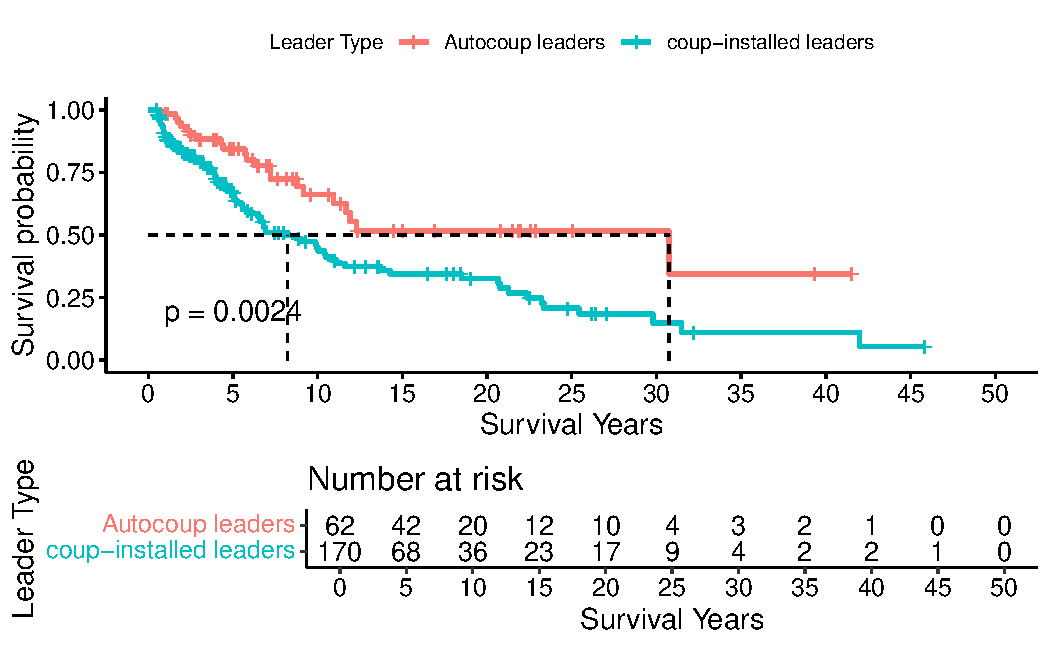
\includegraphics[keepaspectratio]{_coups_and_autocoups_correction_files/figure-pdf/fig-logrank-1.pdf}}

}

\caption{\label{fig-logrank}Survival curves of autocoup and
coup-installed leaders}

\end{figure}%

Preliminary survival analysis, using a log-rank test illustrated in
Figure Figure~\ref{fig-logrank}, reveals a statistically significant
difference in tenure length between these two groups. The survival curve
for autocoup leaders consistently lies above that of coup-installed
leaders, suggesting both a lower hazard of removal and longer durations
in office for the former.

This study posits that the method of power acquisition exerts a
significant influence on leadership survival. Coup-installed leaders may
encounter greater resistance or institutional fragility, contributing to
shorter average tenures than those who consolidate power through
autocoups. Employing Cox proportional hazards and time-dependent Cox
models, the analysis supports this hypothesis by demonstrating that
autocoup leaders tend to remain in office longer than their
coup-installed counterparts.

This research makes two key contributions to the literature on political
survival. First, it introduces an under-explored explanatory factor: the
method of accession to power. Second, by applying survival models, this
study provides robust empirical evidence of the significant disparity in
tenure length between autocoup and coup-installed leaders. These
insights may help account for the rising incidence of autocoup-driven
tenure extensions since 2000, as incumbents increasingly observe and
emulate successful precedents.

The remainder of this chapter is structured as follows: Section 2
reviews the existing literature on political survival, establishing the
theoretical context for the analysis. Section 3 examines the factors
influencing the longevity of coup-installed and autocoup leaders.
Section 4 details the methodological approach and data sources,
including the application of survival analysis techniques. Section 5
presents the empirical findings and interprets their implications.
Finally, Section 6 offers concluding reflections and considers the
broader consequences of the findings for political stability and
democratic development.

\section{Literature review}\label{literature-review}

The longevity of political leaders, which varies markedly across
regimes, countries, and historical periods, has long been a focal point
of inquiry within political science. Research in this field is generally
categorised into two interrelated strands: regime survival and
individual leader survival. While the former concerns the endurance of
political systems---such as monarchies, dominant parties, or ideological
frameworks---the latter focuses on the duration of individual leaders'
tenure in office.

Patterns of political survival differ significantly across regime types.
For instance, parliamentary democracies (e.g., Japan and the United
Kingdom) often witness sustained party dominance alongside frequent
leadership turnover. Similarly, communist regimes (e.g., China) are
typically characterised by stable party control but relatively frequent
changes in leadership. In contrast, presidential systems (e.g., the
United States) and many military regimes tend to exhibit more frequent
changes in both leadership and ruling entity.

The existing literature on leader survival is both extensive and
diverse. Some studies investigate mechanisms that influence leadership
durability within specific regime types, such as democracies
(\citeproc{ref-svolik2014}{Svolik 2014}) or autocracies
(\citeproc{ref-davenport2021}{Davenport, RezaeeDaryakenari, and Wood
2021}). Others attempt to formulate more general theoretical frameworks
applicable across various political systems
(\citeproc{ref-buenodemesquita2003}{Bueno de Mesquita et al. 2003}).
Despite these efforts, the ambition of constructing a universal theory
of leadership survival remains elusive due to the inherent complexities
across regime contexts.

Mechanisms of leadership transition vary substantially between
democracies and autocracies. In autocratic regimes, leadership selection
processes are often closed, with access restricted to a limited elite.
Even when elections are held, meaningful competition is frequently
constrained by structural or legal barriers. The opacity of leadership
transitions in autocracies complicates assessments of popular support
and renders concepts such as selectorates or winning coalitions, as
theorised by Bueno de Mesquita et al.
(\citeproc{ref-buenodemesquita2003}{2003}), difficult to operationalise.

Given these challenges, focusing research on specific categories of
leaders may yield more analytically fruitful outcomes. The study of
irregular leaders---those who ascend to power via coups or extend their
rule through autocoups---offers a compelling line of inquiry due to the
distinctive uncertainty and volatility that characterise their tenures.

Two dominant perspectives have emerged in the literature to explain
leader survival. The first emphasises objective structural factors and
material resources, such as individual competence
(\citeproc{ref-yu2016}{Yu and Jong-A-Pin 2016}), societal stability
(\citeproc{ref-arriola2009}{Arriola 2009}), economic development
(\citeproc{ref-palmer1999}{Palmer and Whitten 1999};
\citeproc{ref-williams2011}{Williams 2011}), natural resource wealth
(\citeproc{ref-smith2004}{Smith 2004};
\citeproc{ref-quirozflores2012}{Quiroz Flores and Smith 2012};
\citeproc{ref-wright2013}{Wright, Frantz, and Geddes 2013}), and
external support (\citeproc{ref-licht2009}{Licht 2009};
\citeproc{ref-wright2008}{Wright 2008}; \citeproc{ref-thyne2017}{C.
Thyne et al. 2017}). The second perspective focuses on subjective
dimensions and strategic choices, including policy decisions, management
of opposition, and mechanisms for consolidating authority
(\citeproc{ref-gandhi2007}{Gandhi and Przeworski 2007};
\citeproc{ref-morrison2009}{Morrison 2009};
\citeproc{ref-escribuxe0-folch2013}{Escribà-Folch 2013};
\citeproc{ref-davenport2021}{Davenport, RezaeeDaryakenari, and Wood
2021}).

Coups, a critical form of irregular leadership transition, have garnered
substantial scholarly attention. Research has examined strategies for
coup prevention (\citeproc{ref-powell2017}{J. Powell 2017};
\citeproc{ref-sudduth2017}{Sudduth 2017}; \citeproc{ref-debruin2020}{De
Bruin 2020}), as well as the effects of coups on leadership trajectories
and the subsequent behaviour of coup leaders
(\citeproc{ref-sudduth2017}{Sudduth 2017};
\citeproc{ref-sudduth2018}{Sudduth and Bell 2018};
\citeproc{ref-easton2018}{Easton and Siverson 2018}).

Despite this body of work, a significant lacuna remains in the
comparative analysis of leadership survival between coup-installed and
autocoup leaders. This study seeks to address this gap by examining and
comparing the tenure lengths of leaders emerging from these two distinct
forms of irregular power acquisition.

By centring its analysis on the survival of coup-installed versus
autocoup leaders, this research aims to enhance our understanding of
political longevity in the context of irregular leadership transitions.
Such a focus promises to yield important insights into the strategic and
structural conditions that underpin leadership durability in diverse
political environments.

\section{Survival dynamics of autocoup and coup-installed
leaders}\label{survival-dynamics-of-autocoup-and-coup-installed-leaders}

The study of leadership survival within political systems poses
significant methodological and conceptual challenges, owing to the
opaque and complex nature of power transitions. These very challenges,
however, underscore the importance of such inquiry, as it illuminates
the often-neglected dynamics of political leadership. While the survival
trajectories of individual leaders vary considerably, discernible
patterns can be identified. Leaders emerging from similar origins or
operating within comparable regime types frequently display analogous
characteristics, thereby enabling systematic and meaningful comparative
analysis.

\subsection{Key definitions and scope}\label{key-definitions-and-scope}

Prior to undertaking a comparative analysis, it is essential to
establish clear definitions of key terms to ensure conceptual clarity
and analytical coherence. The definitions employed in this chapter align
with those presented in Chapter 2.

Autocoup leaders are defined as incumbent rulers who utilise
extra-constitutional measures to prolong their tenure in office. In
contrast, coup-installed leaders are those who ascend to power following
a successful coup, irrespective of whether they personally orchestrated
or participated in the coup. This inclusive definition encompasses both
coup perpetrators and individuals subsequently appointed to lead,
thereby offering a comprehensive perspective on leadership following
violent or forceful regime change.

Three clarifications are warranted in delineating the analytical scope.
First is about the minimum tenure threshold. To facilitate a meaningful
and robust analysis, the study imposes a minimum threshold of six months
in office for both autocoup and coup-installed leaders. This criterion
serves to exclude brief or interim leadership episodes that are less
analytically relevant to the study of survival dynamics, thereby
enhancing the reliability of the findings.

Second is the potential overlap in leadership categories. Some cases may
present ambiguities due to overlapping leadership pathways. A notable
example is Zine El Abidine Ben Ali, who assumed the presidency of
Tunisia in 1987 following a bloodless coup that removed President Habib
Bourguiba on grounds of ill health. In 2002, Ben Ali further
consolidated power through a constitutional referendum that removed term
limits and raised the presidential age cap from 70 to 75 years
(\citeproc{ref-bonci2019}{Bonci and Cavatorta 2019}). This latter
manoeuvre could be construed as an autocoup. Nevertheless, since Ben Ali
initially came to power via the 1987 coup and remained in office
continuously, he is classified in this study as a coup-installed leader.
To preserve analytical consistency and prevent category overlap, this
study adopts the rule that any leader who initially acquires office
through a coup is categorised as coup-installed, even if they later
consolidate or extend their rule through elections or
extra-constitutional means.

Third is the focus on post-event tenure. The analysis compares the
post-autocoup tenure of autocoup leaders with the post-coup tenure of
coup-installed leaders. Any period served by autocoup leaders prior to
the tenure-extending manoeuvre is excluded. This approach ensures a
like-for-like comparison by focusing on the period of leadership
characterised by irregular legitimacy and heightened political
uncertainty. Both categories of leaders share key characteristics---such
as limited institutional legitimacy, increased exposure to instability,
and dependence on coercive or extra-legal mechanisms---which render the
comparison analytically fruitful.

\subsection{Challenges in power
consolidation}\label{challenges-in-power-consolidation}

Both autocoup and coup-installed leaders encounter distinct challenges
in consolidating power, largely arising from the differing intensity of
issues related to illegitimacy, uncertainty, and instability. These
disparities create an uneven political landscape, placing coup-installed
leaders at a marked disadvantage. Table~\ref{tbl-leaders} presents a
comparative overview of the principal characteristics of autocoup and
coup-installed leaders, highlighting these critical differences.

\blandscape

\begin{table}

\caption{\label{tbl-leaders}Main features of autocoup and coup-installed
leaders}

\centering{

\fontsize{12.0pt}{14.4pt}\selectfont
\begin{tabular*}{1\linewidth}{@{\extracolsep{\fill}}>{\raggedright\arraybackslash}p{\dimexpr 112.50pt -2\tabcolsep-1.5\arrayrulewidth}>{\raggedright\arraybackslash}p{\dimexpr 225.00pt -2\tabcolsep-1.5\arrayrulewidth}>{\raggedright\arraybackslash}p{\dimexpr 225.00pt -2\tabcolsep-1.5\arrayrulewidth}}
\toprule
Feature & Autocoup Leader & Coup Entry Leader \\ 
\midrule\addlinespace[2.5pt]
Illegitimacy & Normally attained through
lawful procedures, but
lacking consensus
legitimacy & Blatantly illegal \\ 
Uncertainty & Initially with some certainty, but decreases as the leader's age grows or health worsens & Significant uncertainty initially \\ 
Instability & Relatively stable & Unstable except when a strongman emerges or constitutional institutions are established \\ 
Balance of Power & Generally in a better position of power & Initially unclear and challenging to establish a balance \\ 
\bottomrule
\end{tabular*}

}

\end{table}%

\elandscape

\subsubsection*{Illegitimacy}\label{illegitimacy}
\addcontentsline{toc}{subsubsection}{Illegitimacy}

Although both categories of leaders face legitimacy deficits, the nature
and perception of this deficit vary considerably.

For coup-installed leaders, illegitimacy is overt and unequivocal,
stemming from the direct---often violent---seizure of power. Such abrupt
disruptions to established political norms and institutions elicit
immediate condemnation, both domestically and internationally, and cast
doubt on the regime's authority from the outset.

By contrast, autocoup leaders adopt a more covert and strategic
approach, utilising legal and institutional mechanisms to simulate
democratic legitimacy. Though often superficial, this legalistic veneer
can obscure the authoritarian nature of their actions, offering a
temporary shield from domestic opposition and international scrutiny
while they seek to consolidate power.

\subsubsection*{Uncertainty}\label{uncertainty}
\addcontentsline{toc}{subsubsection}{Uncertainty}

The irregular accession of both types of leaders generates uncertainty
regarding the durability of their rule and the modalities of succession.
However, the nature and sources of this uncertainty differ markedly.

Coup-installed leaders confront a triad of uncertainties. First, the
immediate post-coup environment frequently involves intense power
struggles within the military or ruling coalition, creating ambiguity
over who will ultimately prevail. Second, their tenure is intrinsically
unstable, threatened by internal rivalries, popular mobilisation, or the
prospect of counter-coups. Third, the absence of institutionalised
succession mechanisms exacerbates this unpredictability, heightening the
risk of future instability.

Autocoup leaders, while not entirely insulated from uncertainty,
typically face fewer ambiguities. As incumbents, they retain formal
authority post-autocoup, thereby eliminating immediate succession
questions. Moreover, autocoup leaders often articulate explicit
ambitions to prolong their rule indefinitely, or through gradual
extensions, cultivating an image of continuity. This perceived
stability---whether genuine or contrived---may foster a more predictable
political climate in the short term.

\subsubsection*{Instability}\label{instability}
\addcontentsline{toc}{subsubsection}{Instability}

The combination of legitimacy deficits and enduring uncertainty
inevitably fosters insecurity and a sense of political fragility.
Consequently, both autocoup and coup-installed leaders prioritise
strategies to stabilise their regimes. However, the scale and nature of
these challenges differ.

Coup-installed leaders typically face the formidable task of
reconfiguring political power from the ground up. This often involves
purging opponents, suppressing dissent, and restructuring institutional
frameworks. Such aggressive measures can provoke significant resistance,
alienate potential allies, and incite societal unrest. Moreover, the
imperative to appease powerful domestic and international actors may
force these leaders into precarious compromises that further undermine
their authority.

In contrast, autocoup leaders often benefit from a degree of
institutional continuity and regime loyalty. This relative stability
enables them to pursue consolidation incrementally, reducing the
likelihood of immediate backlash. While opposition may persist, autocoup
leaders are generally less exposed to existential threats in the early
stages of their extended rule, affording them greater latitude to
entrench their authority.

Understanding these contrasting challenges allows for a more refined
appreciation of the strategic environments in which irregular leaders
operate. This comparative lens provides a valuable framework for
analysing the divergent pathways to power consolidation, and the varied
tools and tactics employed by autocoup and coup-installed leaders in
navigating the precarious terrain of non-traditional political
ascension.

\subsection{Empirical evidence and
hypothesis}\label{empirical-evidence-and-hypothesis}

Empirical evidence underscores the relative disadvantage faced by
coup-installed leaders, revealing a complex interplay between historical
patterns, difficulties in consolidating power, and variations in
leadership longevity. This section presents key empirical findings and
introduces the central hypothesis that guides this study.

Data analysis indicates a strong correlation between the frequency of
coup attempts within a given country and the likelihood of future coups.
Notably, more than one-third of all coups since 1950 have taken place in
the ten countries with the highest number of coup attempts
(\citeproc{ref-powell2011}{Powell and Thyne 2011}). This suggests a
self-reinforcing cycle of political instability, in which each
successful coup increases the probability of further attempts, thereby
cultivating an environment of persistent uncertainty for coup-installed
leaders.

The disparity in leadership duration between autocoup and coup-installed
leaders is clearly reflected in survival data. As illustrated in
Figure~\ref{fig-logrank}, leaders who extend their tenure through
autocoups remain in office, on average, approximately five years longer
than those who assume power via coups. This marked difference in tenure
highlights the distinct challenges these two categories of leaders
encounter in retaining power.

The divergent consolidation environments faced by autocoup and
coup-installed leaders contribute to a self-perpetuating cycle with
significant implications for tenure length. Coup-installed leaders
confront acute legitimacy deficits and heightened internal instability;
they often struggle to attract and retain durable support, rendering
them more susceptible to both internal dissent and external pressures.
Their comparatively shorter average tenures reinforce perceptions of
volatility and fragility. Autocoup leaders, by contrast, frequently
benefit from a superficial veneer of legality and enjoy a more
favourable starting position as incumbents. This allows them to
consolidate authority more effectively, cultivate elite and public
support, and reduce the immediate risk of displacement. Their longer
tenures further contribute to perceptions of regime stability. This
cyclical dynamic suggests that the initial method of acquiring or
extending power has long-term implications for a leader's capacity to
maintain their position.

Drawing upon these empirical observations and the theoretical framework
outlined in preceding sections, the following hypothesis is proposed:

\textbf{\emph{H4-1: Political leaders who successfully extend their
tenure through autocoups are more likely to enjoy longer extended
tenures than those who assume office through coups.}}

This hypothesis encapsulates the anticipated effects of the differing
challenges and advantages faced by coup-installed and autocoup leaders.
By empirically testing this claim, the study seeks to assess the impact
of irregular accession mechanisms on leadership survival, thereby
advancing a more nuanced understanding of political durability in
contexts of non-traditional transitions to power.

\section{Research design}\label{research-design-1}

This section outlines the methodological framework employed to test the
hypothesis that autocoup leaders exhibit longer survival times in office
than coup-installed leaders. Survival analysis is utilised to model
leadership tenure, with Cox proportional hazards models employed to
estimate the effects of leader type while controlling for relevant
covariates.

\subsection{Methodology: Survival
analysis}\label{methodology-survival-analysis}

Two variants of the Cox model are employed to analyse the survival
durations of coup-installed and autocoup leaders.

\textbf{Cox proportional hazards (PH) model}: This model incorporates
only time-invariant covariates measured at the time of the leader's
entry into office. It assumes that the effects of these covariates on
the hazard rate remain constant over time.

\textbf{Time-dependent Cox model}: This model allows for the inclusion
of covariates whose values may vary over time, such as indicators of
economic performance and levels of political violence. By incorporating
temporal variation, this model offers a more dynamic and nuanced
analysis of leadership survival.

The Cox model is preferred over the Kaplan-Meier estimator due to its
capacity to account for multiple explanatory variables simultaneously.
Although the Cox model does not directly estimate the expected duration
of tenure, it estimates the hazard ratio, which reflects the relative
risk of being removed from office. A higher cumulative hazard
corresponds to a lower probability of survival, thereby capturing
critical dynamics of leadership vulnerability over time.

\subsection{Data and variables}\label{data-and-variables-1}

The analysis relies on a set of dependent and independent variables,
complemented by a range of controls.

\textbf{Survival Time:} Measured in days, this variable captures the
length of a leader's tenure. For coup-installed leaders, the tenure is
measured from the date of their accession via coup. For autocoup
leaders, it begins on the date their original legitimate term would have
expired. For instance, Vladimir Putin assumed the presidency of Russia
in 2000, stepped down in 2008 after completing two terms, and assumed
the post of prime minister while continuing to exert de facto control.
His post-autocoup tenure, therefore, is coded as beginning in 2008.

\textbf{End Point Status:} This categorical variable indicates how a
leader's tenure ended:

\begin{itemize}
\item
  \textbf{0 = Censored:} Denotes leaders who exited office through
  regular or voluntary means, such as electoral defeat, term expiration,
  voluntary resignation due to health, or natural death.
\item
  \textbf{1 = Ousted:} Denotes leaders who were forcibly removed,
  including through coups, resignations under pressure, or
  assassination.
\end{itemize}

The key independent variable is the leader type, which categorizes
leaders into two distinct groups:

\begin{itemize}
\tightlist
\item
  \textbf{Group A = Autocoup leader}: An incumbent who extends their
  tenure through extra-constitutional means.
\item
  \textbf{Group B = Coup-installed leader}: A leader who assumes power
  through a coup, whether or not they personally participated in its
  execution.
\end{itemize}

This variable serves as the primary explanatory factor, enabling a
direct comparison of survival outcomes between the two categories of
irregular leaders.

Data for the dependent and independent variables are drawn from the
newly constructed autocoup dataset introduced in this study, as well as
the Archigos dataset and the Political Leaders and Alliances Dataset
(PLAD).

To isolate the effect of leader type on survival, the analysis
incorporates a set of control variables, as identified in the autocoup
analysis presented in Chapter 3. These include: regime type which is
categorised as democracy, hybrid regime, or autocracy, to account for
institutional differences that may influence leadership stability;
economic performance, measured through macroeconomic indicators such as
GDP growth, which may affect a leader's ability to retain support;
political violence, captures the extent of civil conflict, repression,
or unrest, which can threaten regime stability and leadership tenure;
population size, controls for structural differences across states that
may impact political dynamics; Polity V scores, feflects the
institutional characteristics and degree of democracy or autocracy
within a regime.

These control variables enhance the comparability and robustness of the
statistical models, ensuring that the estimated effects of leader type
are not confounded by broader political, economic, or demographic
conditions.

\section{Results and discussion}\label{results-and-discussion}

\subsection{Model results}\label{model-results}

Regression results for both the Cox Proportional Hazards (PH) model and
the time-dependent Cox model, estimated using the survival package in R
(\citeproc{ref-survival}{Therneau 2024}), are presented in
Table~\ref{tbl-cox}.

\begin{table}

\caption{\label{tbl-cox}Cox models for survival time of different types
of leaders}

\centering{

\fontsize{12.0pt}{14.4pt}\selectfont
\begin{tabular*}{\linewidth}{@{\extracolsep{\fill}}lcccccccc}
\toprule
 & \multicolumn{4}{c}{\textbf{Cox PH Model}} & \multicolumn{4}{c}{\textbf{Time-dependent Cox Model}} \\ 
\cmidrule(lr){2-5} \cmidrule(lr){6-9}
\textbf{Characteristic} & \textbf{N} & \textbf{Event N} & \textbf{HR}\textsuperscript{\textit{1}} & \textbf{SE} & \textbf{N} & \textbf{Event N} & \textbf{HR}\textsuperscript{\textit{1}} & \textbf{SE} \\ 
\midrule\addlinespace[2.5pt]
{\bfseries Leader Type} &  &  &  &  &  &  &  &  \\ 
    Autocoup leaders & 61 & 21 & 1.00 & — & 559 & 21 & 1.00 & — \\ 
    Coup-installed leaders & 167 & 84 & 1.76** & 0.274 & 1,171 & 80 & 1.31 & 0.275 \\ 
{\bfseries Regime Types} &  &  &  &  &  &  &  &  \\ 
    dominant-party & 48 & 20 & 1.00 & — & 395 & 13 & 1.00 & — \\ 
    military & 38 & 19 & 2.26** & 0.351 & 356 & 36 & 2.06** & 0.356 \\ 
    personal & 64 & 30 & 1.67* & 0.296 & 749 & 43 & 1.55 & 0.327 \\ 
    presidential & 36 & 13 & 1.55 & 0.396 & 98 & 3 & 1.40 & 0.713 \\ 
    parliamentary & 18 & 9 & 2.00 & 0.448 & 27 & 1 & 1.91 & 1.07 \\ 
    other & 24 & 14 & 1.86* & 0.374 & 105 & 5 & 2.59** & 0.557 \\ 
{\bfseries GDP Growth Trend} & 228 & 105 & 0.91 & 1.86 & 1,730 & 101 & 0.07* & 1.72 \\ 
{\bfseries GDP per capita} & 228 & 105 & 0.98 & 0.010 & 1,730 & 101 & 0.98*** & 0.010 \\ 
{\bfseries Population: log} & 228 & 105 & 1.00 & 0.079 & 1,730 & 101 & 0.92 & 0.080 \\ 
{\bfseries Polity 5} & 228 & 105 & 1.00 & 0.031 & 1,730 & 101 & 1.01 & 0.027 \\ 
{\bfseries Political violence} & 228 & 105 & 0.95 & 0.051 & 1,730 & 101 & 1.09** & 0.046 \\ 
\bottomrule
\end{tabular*}
\begin{minipage}{\linewidth}
\textsuperscript{\textit{1}}*p\textless{}0.1; **p\textless{}0.05; ***p\textless{}0.01\\
Abbreviations: HR = Hazard Ratio, SE = Standard Error\\
\end{minipage}

}

\end{table}%

The two models yield divergent findings concerning the central question
of this study. The Cox PH model reveals a marginally statistically
significant relationship between leadership type and the hazard of
removal from office ( \(p < 0.1\) ). Specifically, this model supports
the hypothesis that leaders installed through coups face a 1.78 times
greater hazard of removal compared to those who came to power via
autocoups. However, the time-dependent Cox model, which incorporates
time-varying covariates such as economic performance and political
violence, does not find a statistically significant relationship between
leadership type and survival in office. Given the greater robustness of
the time-dependent specification, the interpretation of the principal
findings is grounded in this model.

According to the time-dependent Cox model, and contrary to the initial
hypothesis and preliminary results, the mode of accession to power does
not significantly influence the tenure of irregularly inaugurated
political leaders once relevant covariates---particularly regime
type---are controlled for. Nevertheless, these results reinforce the
broader conclusion of Chapter 3: that the balance of power,
fundamentally shaped by regime characteristics, is central to both the
seizure and retention of political authority.

In particular, regime type emerges as a statistically significant
determinant of political survival. Leaders in military regimes exhibit a
hazard ratio of 2.06 relative to their counterparts in dominant-party
regimes, suggesting that military leaders are significantly more likely
to be ousted. This implies that, all else being equal, a military leader
faces a \(106\%\) greater risk of removal at any given point compared to
a leader within a dominant-party regime. Leaders operating within
regimes classified as ``Other''---typically encompassing transitional or
provisional arrangements---display an even higher hazard ratio of 2.57,
consistent with the inherent volatility of such political
configurations.

Economic development, proxied by GDP per capita, also exerts a
statistically significant influence. A hazard ratio of 0.95 indicates
that each additional \$10,000 in GDP per capita is associated with a
\(5\%\) reduction in the risk of removal, ceteris paribus. Conversely,
political violence, measured via the violence index, demonstrates a
positive relationship with leader removal: a one-unit increase in the
index raises the hazard of removal by approximately \(9\%\).

Other control variables---including GDP growth, the logarithm of
population size, and Polity V scores---do not reach statistical
significance in the time-dependent Cox model. Although these factors are
theoretically salient and frequently employed in studies of political
survival, their lack of significance in this context suggests that,
under conditions of irregular leadership transitions, more immediate
variables such as regime type and political violence may play a more
decisive role. It is plausible that the effects of structural economic
growth, demographic scale, and institutional quality are either mediated
through more proximate mechanisms or unfold over longer time horizons,
rendering them less visible in short- to medium-term analyses of leader
tenure.

It is important to note that the results are contingent upon the
exclusion of very short-lived leaders---those who remained in office for
fewer than 180 days following a coup or autocoup. A significant number
of coup-installed leaders survive only for brief periods---often mere
days or months---a phenomenon that is comparatively rare among autocoup
leaders. Consequently, the exclusion criterion introduces a slight bias
in favour of coup-installed leaders. Nevertheless, this study contends
that the inclusion of such short-lived tenures would be methodologically
inappropriate. Although these leaders technically meet the minimal
threshold for a successful coup (i.e., retaining power for more than
seven days), their failure to consolidate authority suggests they did
not truly succeed in establishing post-coup rule in a meaningful or
sustained manner.

\subsection{Discussion}\label{discussion}

\begin{figure}

\begin{minipage}{0.50\linewidth}

\centering{

\pandocbounded{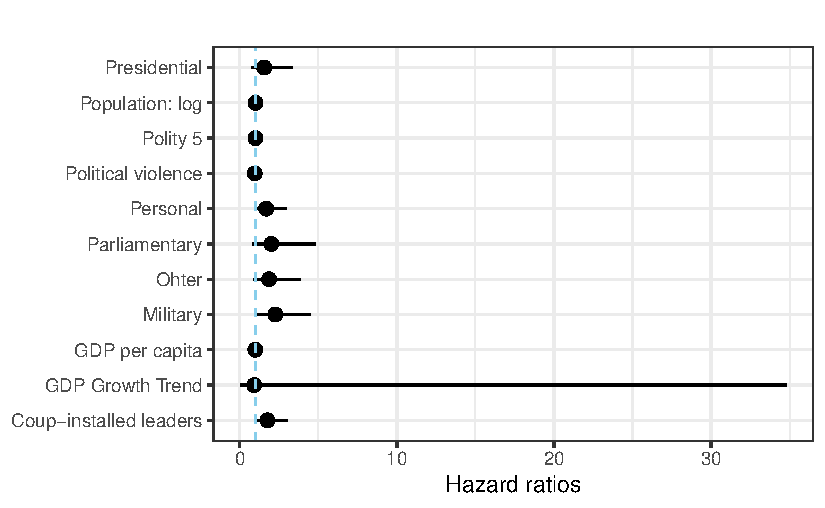
\includegraphics[keepaspectratio]{_coups_and_autocoups_correction_files/figure-pdf/fig-coxHR-1.pdf}}

}

\subcaption{\label{fig-coxHR-1}Cox PH Model}

\end{minipage}%
%
\begin{minipage}{0.50\linewidth}

\centering{

\pandocbounded{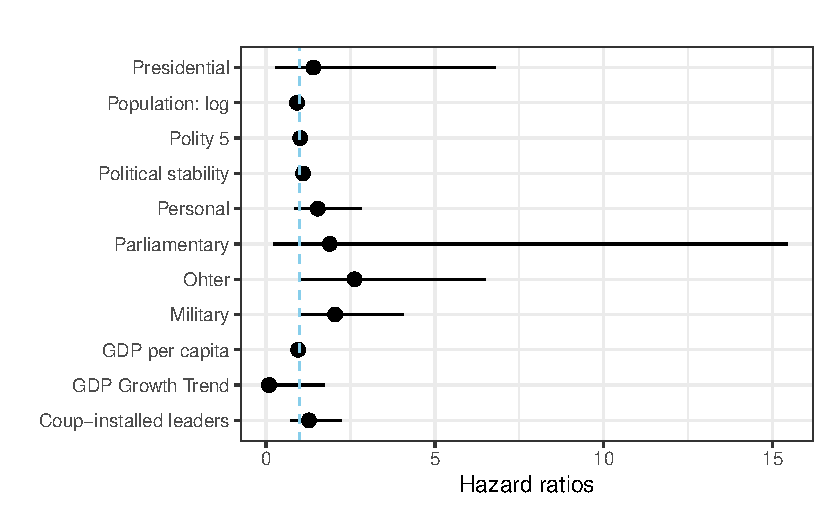
\includegraphics[keepaspectratio]{_coups_and_autocoups_correction_files/figure-pdf/fig-coxHR-2.pdf}}

}

\subcaption{\label{fig-coxHR-2}Time-dependent Cox Model}

\end{minipage}%

\caption{\label{fig-coxHR}Hazard ratios and 95\% CIs for Leader Ousting}

\end{figure}%

Figure~\ref{fig-coxHR} illustrates the hazard ratios and their
associated 95\% confidence intervals for the variables included in the
Cox proportional hazards model. The proximity of each hazard ratio
(represented by a dot) to 1 denotes minimal effect on the risk of
removal from office; a hazard ratio of 1 indicates no effect. The
horizontal lines denote the \(95\%\) confidence intervals, and variables
whose intervals cross the vertical reference line at 1 are not
statistically significant at the \(5\%\) level.

As previously discussed, the hazard ratios for leaders in military
regimes and ``Other'' regimes are both substantially above 1 and
statistically significant at the \(5\%\) level, confirming their
heightened vulnerability to removal. GDP per capita also attains
statistical significance, albeit with a hazard ratio very close to 1,
indicating a relatively modest substantive effect.

Although the hazard ratios for GDP growth and regime type (e.g.,
presidential or parliamentary) appear visually distant from 1, their
respective confidence intervals intersect the vertical line, indicating
a lack of statistical significance at conventional thresholds.

Most other variables display hazard ratios close to 1, suggesting that
marginal changes in these predictors do not substantially alter the
likelihood of political removal for leaders emerging from coups or
autocoups.

\subsection{Assessing the proportional hazards
assumption}\label{assessing-the-proportional-hazards-assumption}

Evaluating the proportional hazards assumption is essential to ensure
the validity of the Cox model estimates. This assumption was tested
using a chi-squared test based on Schoenfeld residuals, which assesses
whether the effects of covariates remain constant over time. The results
indicate that neither the standard Cox PH model nor the time-dependent
Cox model violates this assumption. The global p-values---0.12 for the
standard model and 0.23 for the time-dependent model---exceed the
conventional \(5\%\) significance threshold, thereby confirming that the
proportional hazards assumption holds in both cases.

\section{Summary}\label{summary-2}

This chapter has examined the survival durations of political leaders
who assumed office through irregular means---specifically coups and
autocoups---by employing survival analysis techniques, including the Cox
proportional hazards model and a time-dependent Cox model. While the
standard Cox model indicated a marginally significant difference in the
risk of removal between autocoup and coup-installed leaders, this
association did not attain statistical significance in the
time-dependent model, which offers a more rigorous specification by
accounting for time-varying covariates.

The findings suggest that, once regime type and other pertinent
covariates are controlled for, the method of accession---whether via
coup or autocoup---does not independently determine leader survival.
Rather, regime type emerges as a key determinant. Leaders operating
within military or transitional (``other'') regimes face significantly
higher risks of removal than those in dominant-party systems.
Furthermore, economic development, as measured by GDP per capita, and
political violence significantly influence tenure length, whereas GDP
growth, population size, and democratic quality (as captured by Polity V
scores) do not exhibit statistically significant effects.

These results reinforce the central argument that institutional
context---particularly regime characteristics---plays a more decisive
role in shaping political longevity than the initial method of seizing
power. This conclusion is consistent with earlier qualitative
assessments and underscores the importance of integrating institutional
and structural variables into analyses of political survival.

Methodologically, the chapter illustrates the utility of time-dependent
modelling in political science, particularly where covariates evolve
over time. It also contributes to the emerging literature on autocoups
by offering one of the first systematic empirical assessments of their
implications for political survival. However, reliance on a newly
constructed dataset for autocoups introduces certain limitations,
underscoring the need for further refinement and expansion in future
research.

In sum, this chapter provides empirical evidence supporting the
proposition that regime characteristics, more than the mode of accession
alone, shape the durability of irregular political leadership. These
insights contribute to broader debates on authoritarian resilience,
democratic backsliding, and the institutional foundations of political
authority.

\chapter{Coups, Autocoups, and
Democracy}\label{coups-autocoups-and-democracy}

\section*{Abstract}\label{abstract-4}
\addcontentsline{toc}{section}{Abstract}

This chapter explores the impact of autocoups on political institutions,
drawing comparisons with traditional coups through an analysis of
changes in Polity scores. I contend that, first, incumbent leaders
frequently consolidate power by undermining established institutions in
anticipation of an autocoup, resulting in a decline in Polity scores
even prior to the event. Second, unlike coups, which produce mixed
outcomes regarding democratization, autocoups almost invariably lead to
democratic backsliding or authoritarian entrenchment, as they are
specifically designed to dismantle institutional checks, enabling
leaders to maintain power for significantly longer periods than those
installed via coups.

Employing a country-fixed effects model and utilizing datasets on both
autocoups and coups, this study reveals that Polity scores decline both
preceding and following an autocoup, while coups tend to trigger an
immediate decrease that may allow for some degree of democratic recovery
over time. These findings underscore the divergent political
trajectories associated with coups and autocoups. This research not only
addresses a critical gap in the empirical analysis of autocoups but also
significantly raises awareness within academic and policy-making circles
regarding their potential adverse effects, including democratic
backsliding and further authoritarian deterioration.

\section{Introduction}\label{introduction-4}

In the preceding chapters, I clarified the definition of an autocoup,
introduced a novel dataset on autocoups, conducted empirical analyses on
the determinants of autocoup attempts, and compared the post-event
survival times of leaders established through coups versus autocoup
leaders. A natural follow-up question emerges: What are the broader
impacts of autocoups? Specifically, from a political science
perspective, how do autocoups affect the process of democratization?

As previously noted, due to the absence of a widely recognized dataset
on autocoups, most existing discussions on their impact have relied on
case studies (\citeproc{ref-baturo}{Baturo and Elgie, n.d.};
\citeproc{ref-baturo2022}{Baturo and Tolstrup 2022}). To move beyond
case-specific analyses and adopt a more systematic and comparative
approach, this chapter aims to pioneer empirical research on the
democratic consequences of autocoups. The first objective of this
chapter, therefore, is to examine whether autocoups reinforce
authoritarianism, promote democratization, or have no significant effect
on political regimes.

Given the conceptual and empirical connections between coups and
autocoups, another key objective is to compare their respective effects
on democratization. While both events disrupt existing political orders,
their immediate and long-term consequences may vary significantly.
Understanding these distinctions is essential for evaluating their
broader implications.

To address these questions, this study leverages data from a widely
recognized coup dataset alongside a newly compiled dataset on autocoups.
Employing a fixed-effects model, it evaluates their effects on
democracy, as measured by the Polity Index. The findings reveal that
both coups and autocoups lead to an immediate decline in democratic
levels. However, coups have a more pronounced negative short-term
impact. Notably, three years after these events, democracies affected by
coups tend to show significant recovery, whereas those experiencing
autocoups exhibit no meaningful improvement.

This study offers two significant contributions to the field of
political science. First, it provides the inaugural empirical analysis
of the impact of autocoups on democratization, effectively addressing a
critical gap in the existing literature. Second, by directly comparing
the effects of coups and autocoups, this research highlights autocoups
as a distinct phenomenon that demands increased scholarly inquiry and
policy focus.

The remainder of this chapter is structured as follows: Section 2
analyzes the impact of autocoups on democratization, by comparing the
effects with traditional coups. Section 3 outlines the research design,
methodology, and variables used in this study. Section 4 presents and
interprets the empirical findings, followed by a discussion of their
implications. Finally, Section 5 concludes by summarizing the key
results and exploring their significance for understanding and
mitigating the occurrence of autocoups.

\section{Impact of autocoups on political
change}\label{impact-of-autocoups-on-political-change}

According to the definition in Chapter 2, an autocoup refers to an
incumbent leader extending their tenure in power beyond the originally
mandated limits, whether through legal or illegal means. While the
leader may assume a different title or position, the individual in power
remains unchanged. Therefore, unlike traditional coups, an autocoup does
not result in real leadership turnover, elite restructuring, or regime
change. In other words, the fundamental ruling structure remains intact.

This distinction has important implications. Since regime change rarely
occurs following an autocoup, its impact on politics cannot be assessed
using conventional methods. Typically, studies on coups and
democratization measure their effects by estimating the probability of
regime transition---either from autocracy to democracy or vice
versa---as seen in previous research on coup outcomes
(\citeproc{ref-thyne2014}{C. L. Thyne and Powell 2014};
\citeproc{ref-derpanopoulos2016}{Derpanopoulos et al. 2016};
\citeproc{ref-miller2016}{Miller 2016}). However, this approach is not
suitable for autocoups, as they do not directly trigger regime
transfers.

Although autocoups rarely lead to formal regime change, this does not
mean they have no impact on political dynamics. In fact, they inevitably
shape political trajectories in various ways and, on occasion, can even
lead to significant transformations. Therefore, a more appropriate
method for assessing the political impact of autocoups is to analyze
democratic indices, such as those measured by Polity5
(\citeproc{ref-p1}{Monty G. Marshall and Gurr 2020}). The Polity Score,
ranging from -10 (full autocracy) to +10 (full democracy), captures
gradual shifts in political regime characteristics rather than abrupt
transitions. Thus, even if an autocoup does not result in a formal
regime change, subtle shifts in political openness and institutional
constraints can still be assessed by examining variations in Polity
scores before and after the event. This approach has also been employed
in previous studies (\citeproc{ref-dahl2023}{Dahl and Gleditsch 2023}).

Although autocoups may not lead to significant regime change, their
impact on democratization should not be overlooked. However, their
influence differs from that of traditional coups in at least two key
ways.

\subsection{\texorpdfstring{\textbf{The pre-emptive effects of autocoups
on political
dynamics}}{The pre-emptive effects of autocoups on political dynamics}}\label{the-pre-emptive-effects-of-autocoups-on-political-dynamics}

First and foremost, unlike coups, which are marked by clear, decisive
events---such as the removal of a leader---autocoups typically unfold
gradually, through incremental steps rather than a singular, dramatic
event. Incumbent leaders seeking to extend their tenure often lay the
groundwork well in advance before executing their final move to remain
in power. To reduce resistance and opposition, they engage in extensive
preparation, which may include purging officials, suppressing political
opposition, cracking down on dissent and protests, and restricting press
freedom. Without such measures, an autocoup might face strong internal
resistance, and in the worst case, provoke a backlash that not only
derails the leader's attempt to extend their rule but also results in
their immediate removal from office.

However, once an incumbent successfully secures an extension of their
rule, continued repression is not always necessary. On the contrary,
some leaders relax political pressure to ease internal dissent and
mitigate opposition from external actors. This adaptive approach helps
maintain stability after the autocoup is complete.

As a result, the primary impact of autocoups on political change is
often reflected in shifts in political scores before the final stage of
the autocoup is enacted. Once the process is completed, further shifts
may be minimal. In contrast, coup plotters, unlike incumbents, lack the
ability to influence political institutions beforehand, meaning their
impact on politics is often felt in the aftermath rather than before the
event.

This distinction is evident in empirical cases of autocoups.

One of the most frequently cited examples of an autocoup is Peru's 1992
case, in which President Alberto Fujimori dissolved Congress,
temporarily suspended the 1979 Constitution, and ruled by decree until
November of that year, when a \emph{Democratic Constituent Congress} was
elected to draft a new constitution (\citeproc{ref-cameron1998}{Maxwell
A. Cameron 1998b}). However, these moves did not immediately grant
Fujimori a longer tenure in office.

Under the 1979 Peruvian Constitution, immediate presidential re-election
was prohibited. To bypass this restriction, Fujimori initiated a
constitutional overhaul, leading to the adoption of a new constitution
in 1993, which permitted re-election. Consequently, he secured a second
term in 1995 (\citeproc{ref-baturo2019}{Baturo 2019}).

An analysis of Peru's Polity5 scores during this process reflects these
political changes. Upon taking office in 1990, Peru's Polity score was
8, remaining unchanged in 1991. However, a dramatic shift occurred in
1992, when Fujimori dissolved Congress, causing the Polity score to
plummet from 8 to -4. Interestingly, when he formally extended his rule
by amending the constitution in 1993, the score rebounded slightly to
-1. This -1 score remained unchanged throughout Fujimori's tenure until
2000, indicating a lack of further institutional transformation after
the constitutional amendment.

A similar pattern emerges in Belarus under Alexander Lukashenko. Upon
assuming office as president in 1994, Belarus had a Polity5 score of 8.
However, in 1995, when Lukashenko moved to hold a referendum---defying
opposition in the Supreme Council and threatening to suspend its
activities---the score dropped sharply to 0. Following the 1996
referendum, which extended his term by two additional years, Lukashenko
officially overstayed his tenure. Consequently, the Polity5 score
further declined to -7 in 1996, where it has remained ever since,
despite two additional term extensions (\citeproc{ref-ash2014}{Ash
2014}; \citeproc{ref-baturo}{Baturo and Elgie, n.d.}).

These cases illustrate a broader pattern: the impact of autocoups on
political change is often reflected before the final stage of the
autocoup is enacted, whereas the impact of coups tends to materialize
afterwards, as have been fully discussed by previous studies.

Based on this analysis, I propose the first hypothesis:

\begin{quote}
\emph{H1}: Autocoups primarily shape political change in advance,
whereas coups typically drive political change only after they are
executed.
\end{quote}

\subsection{\texorpdfstring{\textbf{The singular nature of
autocoups}}{The singular nature of autocoups}}\label{the-singular-nature-of-autocoups}

Secondly, in contrast to the ambiguous nature of coups
(\citeproc{ref-dahl2023}{Dahl and Gleditsch 2023}), the impact of
autocoups on political change rarely contributes to democratization.

The influence of coups on democratization has been extensively examined
in existing literature. Some scholars argue that coups---and even the
mere threat of them---can act as catalysts for democratization. One
argument suggests that coups deliver a political ``shock'' that may
create opportunities for liberalization that would not have otherwise
materialized (\citeproc{ref-thyne2014}{C. L. Thyne and Powell 2014}). In
a critical examination, Derpanopoulos et al.
(\citeproc{ref-derpanopoulos2016}{2016}) questioned the role of coups in
promoting democracy, engaging in multiple rounds of debate with Miller
(\citeproc{ref-miller2016}{2016}). More recently, Dahl and Gleditsch
(\citeproc{ref-dahl2023}{2023}) further explored this ongoing
discussion, arguing that both democratic and autocratic transitions are
likely to follow a coup, with popular mobilization playing a decisive
role in shaping post-coup trajectories.

A frequently cited example of a ``pro-democracy coup'' occurred in
February 2010, when Nigerien troops ousted President Mamadou Tandja
after he extended his rule autocratically. The Supreme Council for the
Restoration of Democracy (CSRD) took control, pledging democratic
reforms. Their actions were widely celebrated, with both citizens and
political opposition viewing the coup as an opportunity to restore
democracy. The CSRD fulfilled its commitment by overseeing free and fair
elections in 2011, resulting in Mahamadou Issoufou assuming the
presidency (\citeproc{ref-miller2016}{Miller 2016}).

While the debate on the democratic consequences of coups remains
ongoing, it is evident that their impact is not uniform. In contrast,
autocoups almost never lead to democratic transitions, nor do they even
marginally enhance political freedoms. This stems from the intrinsic
nature of autocoups, which disrupt the established process of political
leadership transition, particularly term limits.

Term limits are constitutional provisions that restrict the maximum
duration a leader can remain in office. They play a crucial role in both
democracies and autocracies by preventing the excessive concentration of
power and ensuring political stability. In democracies, term limits
promote accountability, leadership renewal, and reduce the risks of
corruption and authoritarian entrenchment. In autocracies, when
enforced, they can curb indefinite rule, mitigate succession crises, and
provide rare opportunities for political transitions. However, without
term limits, leaders can entrench themselves in power, undermining
institutions and hindering political progress.

As shown in Table~\ref{tbl-autocoup_method} in Chapter 3, autocoups are
executed through either façade legal mechanisms or blatantly illegal
methods. This includes amending or disregarding term limits, delaying or
cancelling elections, rigging electoral outcomes, or outright refusing
to accept election results. While many autocoups maintain a veneer of
legality, their defining characteristic is the violation of term limits,
which are intended as safeguards against prolonged and unchecked rule.

As previously discussed, before an incumbent leader formally overstays
their term, they often inflict significant damage on political
institutions. Furthermore, to secure their prolonged rule, they are
unlikely to fully restore political freedoms even if they temporarily
ease political repression once they have consolidated power.

Case studies from Peru and Belarus illustrate how autocoups lead to a
decline in Polity scores, reflecting democratic backsliding. However,
most autocoups occur in already autocratic regimes where Polity scores
are low. This aligns with trends observed in coups, which also primarily
occur in autocracies.

For instance, in China's 2018 constitutional amendment, Xi Jinping
abolished presidential term limits, effectively allowing himself to
remain in power indefinitely\footnote{\textbf{BBC News,} ``China's Xi
  Allowed to Remain `President for Life' as Term Limits Removed,''
  \emph{BBC News}, March 11, 2018,
  \url{https://www.bbc.co.uk/news/world-asia-china-43361276}, accessed
  March 14, 2025.}. However, China's Polity score remained unchanged at
-7 before and after the amendment. This pattern is common in autocratic
regimes with Polity scores below -6, as they already lack significant
democratic features, leaving little room for further decline.

While most autocoups occur in low-Polity-score countries, some have
taken place in relatively democratic settings, where the Polity score
remains stable despite term limit extensions. This is particularly
evident in Latin America, where presidents have amended ``no immediate
re-election'' rules to allow for a second consecutive term, but
voluntarily stepped down afterwards. Examples include: Argentina (1993),
Polity score remained at 7; Brazil (1997), Polity score remained at 8,
Colombia (2004), Polity score remained at 7. In these cases, leaders
extended their tenure within a structured political framework without
further dismantling democratic institutions
(\citeproc{ref-baturo2019}{Baturo 2019}).

Across all cases---whether in Peru, Belarus, China, Argentina, Brazil,
or Colombia---there is no instance where a Polity score increased
following an autocoup. In the autocoup dataset which I introduced in
Chapter 3, only four cases---Guinea-Bissau (1988), Burkina Faso (1997),
Congo-Brazzaville (2001), and Lebanon (2004)---saw minor increases in
Polity scores, but the changes were insignificant.

Thus, unlike some coup leaders who justify their actions by claiming to
restore democracy (as seen in Niger's 2010 case), leaders who execute
autocoups lack any democratic justification. If their true intention
were to advance democracy, they would transfer power peacefully rather
than violate term limits.

Based on this analysis, I propose the second hypothesis:

\begin{quote}
\emph{H2}: Autocoups are more likely to entrench autocracy than coups.
\end{quote}

\section{Methodology and variables}\label{methodology-and-variables}

\subsection{Methodology}\label{methodology-1}

As discussed earlier, autocoups are less likely to result in full regime
transitions---either from democracy to autocracy or vice versa.
Therefore, it is inappropriate to assess their effects solely based on
regime transitions or changes that cross a critical threshold. Instead,
this study examines political changes through fluctuations in Polity5
scores.

Unlike coup analysis, which primarily focuses on post-event effects,
this study examines both pre-event and post-event impacts of autocoups.
Specifically, pre-event effects are measured by the change in Polity5
scores three years before the autocoup compared to the year of the
autocoup, expressed as:

\(Polity_t - Polity_{t-3}\)

Post-event effects are measured by the change in Polity5 scores three
years after the autocoup compared to the year of the autocoup, expressed
as:

\(Polity_{t+3} - Polity_t\)

The three-year window is chosen for two key reasons. Pre-event political
changes typically occur incrementally, as incumbents consolidate power
gradually over several years rather than through a single, abrupt
action. Post-event analysis focuses on medium-term effects rather than
short-term shocks, as autocoups rarely trigger immediate regime
transitions and instead reinforce existing political structures.
Short-term fluctuations may be too minor to capture meaningful
institutional change empirically.

To estimate how political institutions change before and after
autocoups, I employ a linear model with country-case fixed effects. For
pre-event effects, I analyze attempted autocoups, since before the
event, no one knows whether the autocoup will succeed or fail.

For post-event effects, I analyze only successful autocoups for three
reasons: The majority of autocoups succeed (87 out of 110 cases); failed
autocoups tend to produce immediate political shocks, rather than
medium- or long-term effects; failed autocoups are often followed by
major disruptive events, such as coups, insurrections, or mass protests,
making it difficult to isolate their impact. For example, in Niger's
case, a failed autocoup in 2009 was followed by a coup in 2010, creating
overlapping political effects. In contrast, successful autocoups provide
a clearer analytical framework, as their effects are less entangled with
other disruptions, allowing for a more systematic assessment of
institutional change.

\subsection{Variables}\label{variables}

This study uses a global sample of all country-year data from 1950 to
2020, applying a linear model to examine the effects of autocoups on
political change. The dependent variable is the change in Polity scores,
while the main independent variable is autocoups. The dataset includes
approximately 7,500 observations.

The dependent variable measures political change using three-year
differences in Polity scores. Model 1 (Pre-event effects):
\(Polity_t − Polity_{t − 3}\). Model 2 (Post-event effects):
\(Polity_{t+3} - Polity_t\).

The Polity score ranges from -10 (full autocracy) to 10 (full
democracy). Some values in the dataset, such as -66, -77, and -88,
represent transitional regimes or special periods. To prevent excessive
data loss, I replace these values with the closest valid Polity scores.
This approach ensures that the model captures all changes in Polity
scores, rather than focusing solely on transitions that cross a
democratic threshold.

The main independent variable is autocoups, as introduced in Chapter 3.
The dataset includes110 attempted autocoups (used for pre-event
analysis) and 87 successful autocoups (used for post-event analysis).
For pre-event analysis, the autocoup variable is binary, where: 1
indicates the presence of an attempted autocoup and 0 indicates no
autocoup event.

For post-event analysis, I apply decay functions to account for both
immediate and delayed effects, following the methodology of Dahl and
Gleditsch (\citeproc{ref-dahl2023}{2023}). To assess the persistence of
autocoup effects, I consider a half-life specification of five years,
analysing the impact from the autocoup year (\(y_t\)) to four years
after (\(y_{t+4}\)).

I also include traditional coups as a secondary independent variable for
two reasons. Comparative significance: It is essential to compare the
effects of autocoups and coups. Overlapping events: In many cases, coups
and autocoups are interconnected, as autocoups can trigger coups.
Distinguishing their effects is necessary for a clear empirical
analysis.

As in previous chapters, I use the coup dataset from Powell and Thyne
(\citeproc{ref-powell2011}{2011}). To maintain consistency, I apply the
same methodological approach to coups as to autocoups: Binary coding for
pre-event effects and decay function coding for post-event effects.

Control variables include economic performance, political violence, and
population size, all of which have been analysed in previous chapters.
Additionally, I incorporate two dummy variables. The first,
\textbf{``\textbf{non\_democracy},''} accounts for regime type,
recognizing that non-democratic regimes with Polity scores below -6 have
limited room for further decline, while democracies with scores above 6
are less likely to experience significant increases. The second,
\textbf{``\textbf{cold\_war},''} follows the approach used in prior
studies on the impact of coups on democratization
(\citeproc{ref-thyne2014}{C. L. Thyne and Powell 2014};
\citeproc{ref-derpanopoulos2016}{Derpanopoulos et al. 2016};
\citeproc{ref-dahl2023}{Dahl and Gleditsch 2023}) and accounts for the
Cold War period. This variable captures the observable trend of
declining Polity scores from the 1960s to 1990, followed by an upward
shift after 1990.

\section{Results and discussion}\label{results-and-discussion-1}

\subsection{Pre-event effects}\label{pre-event-effects}

Initially, I analyse the trajectory of Polity scores leading up to these
events. As presented in Table~\ref{tbl-demomodel}, columns 1 and 2
display the empirical results for pre-event effects, examining changes
over two years (model 1) and three years (model 2) prior to the event.
Consistent with the first hypothesis, Polity scores exhibit a
significant decline in the 2--3 years preceding an autocoup. Notably,
this downward trend is both more pronounced and statistically
significant for autocoups compared to traditional coups.

\begin{table}

\caption{\label{tbl-demomodel}The Impact of Autocoups on
Democratization(1950--2018): OLS with country-fixed effects}

\centering{

\begin{tabular}{@{\extracolsep{30pt}}lcccc} 
\\[-1.8ex]\hline 
\hline \\[-1.8ex] 
 & \multicolumn{4}{c}{Dependent variable: Differences of Polity scores} \\ 
\cline{2-5} 
\\[-1.8ex] & \multicolumn{2}{c}{Pre-event effects} & \multicolumn{2}{c}{Post-event effects} \\ 
\\[-1.8ex] & (1) & (2) & (3) & (4)\\ 
\hline \\[-1.8ex] 
 Autocoup & $-$0.487$^{*}$ & $-$1.802$^{***}$ & $-$0.109 & $-$0.168 \\ 
  & (0.286) & (0.340) & (0.176) & (0.198) \\ 
  & & & & \\ 
 Coup & 0.011 & $-$1.276$^{***}$ & 0.479$^{***}$ & 0.715$^{***}$ \\ 
  & (0.129) & (0.153) & (0.077) & (0.104) \\ 
  & & & & \\ 
 GDP per Capita & $-$0.005$^{***}$ & $-$0.007$^{***}$ & $-$0.007$^{***}$ & $-$0.007$^{***}$ \\ 
  & (0.002) & (0.002) & (0.002) & (0.002) \\ 
  & & & & \\ 
 Economic Trend & $-$0.703$^{*}$ & $-$1.240$^{***}$ & $-$0.942$^{**}$ & $-$1.030$^{**}$ \\ 
  & (0.388) & (0.462) & (0.464) & (0.463) \\ 
  & & & & \\ 
 Log Population & 0.682$^{***}$ & 1.013$^{***}$ & 1.163$^{***}$ & 1.154$^{***}$ \\ 
  & (0.099) & (0.119) & (0.119) & (0.119) \\ 
  & & & & \\ 
 Political Violence & 0.016 & 0.028 & 0.020 & 0.021 \\ 
  & (0.020) & (0.023) & (0.023) & (0.023) \\ 
  & & & & \\ 
 Non-Democracy & 1.682$^{***}$ & 2.443$^{***}$ & 2.411$^{***}$ & 2.428$^{***}$ \\ 
  & (0.087) & (0.104) & (0.105) & (0.105) \\ 
  & & & & \\ 
 Cold War & $-$0.256$^{***}$ & $-$0.261$^{**}$ & $-$0.250$^{**}$ & $-$0.259$^{**}$ \\ 
  & (0.088) & (0.104) & (0.104) & (0.104) \\ 
  & & & & \\ 
\hline \\[-1.8ex] 
Observations & 8,926 & 8,761 & 8,761 & 8,761 \\ 
R$^{2}$ & 0.049 & 0.082 & 0.076 & 0.077 \\ 
Adjusted R$^{2}$ & 0.030 & 0.063 & 0.057 & 0.058 \\ 
F Statistic & 56.188$^{***}$ & 96.025$^{***}$ & 87.952$^{***}$ & 89.142$^{***}$ \\ 
\hline 
\hline \\[-1.8ex] 
\textit{Note:}  & \multicolumn{4}{r}{$^{*}$p$<$0.1; $^{**}$p$<$0.05; $^{***}$p$<$0.01} \\ 
\end{tabular}

}

\end{table}%

Column 1 examines the pre-event changes, specifically the difference
between Polity scores at time \(t-1\) and \(t-3\)
(\(Polity_{t-1} - Polity_{t-3}\)). The results reveal a statistically
significant decrease in Polity scores prior to autocoups. On average,
Polity scores decline by 0.45 in the two years before an autocoup,
holding other factors constant. In contrast, no significant changes are
observed before traditional coups, indicating that pre-coup periods do
not measurably affect democratization levels.

Column 2 assesses the cumulative impact from three years prior to the
event year, calculated as \(Polity_{t} - Polity_{t-3}\). As previously
discussed, the year of an autocoup or coup witnesses a substantial shock
to political institutions. Consequently, both types of events result in
a decline in Polity scores relative to three years earlier. However, the
negative effect of autocoups is more severe. Polity scores decline by an
average of 1.53 in the three years leading up to an autocoup, compared
to 1.27 for coups, all else being equal. This disparity reinforces our
hypothesis that autocoups have a more detrimental pre-event effect on
democratic institutions as incumbents overextend their legitimate
tenure.

\subsection{Post-event effects}\label{post-event-effects}

Columns 3 and 4 present the empirical results for post-event effects,
analysing changes in Polity scores following attempted (column 3) and
successful (column 4) autocoups.

Column 3 examines the impact of attempted autocoups. The results
indicate that attempted autocoups do not have a statistically
significant effect on Polity scores. This contrasts with coup attempts,
which lead to an average increase of 0.48 in Polity scores over three
years, all else being equal.

Column 4 evaluates the impact of successful autocoups. In contrast to
attempted autocoups, successful autocoups demonstrate a significant
negative effect on Polity scores, with an average decline of 0.33 over
three years, holding other factors constant. Conversely, successful
coups continue to exhibit positive effects on democratization, resulting
in an average increase of 0.72.

These findings yield several key insights. First, while both successful
and attempted coups influence Polity scores, only successful autocoups
produce statistically significant effects---and exclusively in a
negative direction. Second, the impact of coups on democratization is
more nuanced. Although post-coup Polity scores may improve, the pre-coup
period often involves significant democratic backsliding. My models
indicate that, on average, the democratic gains following a coup fail to
offset the losses incurred before it.

\subsection{Effects of control
variables}\label{effects-of-control-variables}

To ensure robust results, I incorporated several control variables into
the models. While economic trends and political violence do not exhibit
statistically significant effects on Polity scores, other factors
warrant further discussion.

The impact of the Cold War is relatively straightforward. As outlined in
the research design section, global democracy experienced a general
decline during the Cold War period. Consistent with this trend, all four
models indicate that the Cold War era is associated with an average
decrease of 0.23 in Polity scores.

The effects of GDP per capita, population size, and regime type,
however, present a more complex pattern. Counter-intuitively, higher GDP
per capita correlates with lower Polity scores, whereas non-democratic
regimes and larger populations correspond with positive changes in
Polity scores. This pattern may be explained by considering baseline
differences between democracies and non-democracies. In established
democracies, Polity scores are already high, leaving limited room for
further increases. These countries also tend to have higher GDP per
capita and lower birth rates, further reinforcing stability in their
democratic scores. In contrast, non-democracies start from lower Polity
scores, providing greater potential for upward movement. Given that
authoritarian regimes often exhibit weaker economic performance and
higher population growth rates, their Polity scores may increase as they
undergo political transitions or reforms.

Taken together, these results support both hypotheses. First, the
primary effects of autocoups on Polity scores manifest before the events
occur. Second, whereas coups have ambiguous consequences for
democratization, the effects of autocoups are
unidirectional---consistently negative.

\subsection{Robustness tests}\label{robustness-tests}

To assess the sensitivity of my key findings to model specifications, I
conduct a series of robustness tests. The results indicate that the
findings remain consistent across these variations.

First, I compare the effects of autocoups over a period ranging from one
to five years after the event. The results show that the effects of
coups are positive and statistically significant throughout all five
years, with a general trend of increasing magnitude as time progresses.
In contrast, the effects of autocoups are negative across all five years
but reach statistical significance only three years after the event.
This finding aligns with the earlier hypothesis: autocoups never
contribute to an increase in Polity scores.

\begin{table}

\caption{\label{tbl-demomodel1}The Impact of Autocoups on
Democratization: one to five years}

\centering{

\begin{tabular}{@{\extracolsep{10pt}}lccccc} 
\\[-1.8ex]\hline 
\hline \\[-1.8ex] 
 & \multicolumn{5}{c}{Dependent variable: Differences of Polity scores} \\ 
\cline{2-6} 
\\[-1.8ex] & \multicolumn{5}{c}{Years after the event} \\ 
\\[-1.8ex] & (1) & (2) & (3) & (4) & (5)\\ 
\hline \\[-1.8ex] 
 Autocoup & $-$0.082 & $-$0.101 & $-$0.168 & $-$0.284 & $-$0.355 \\ 
  & (0.119) & (0.165) & (0.198) & (0.227) & (0.247) \\ 
  & & & & & \\ 
 Coup & 0.192$^{***}$ & 0.436$^{***}$ & 0.715$^{***}$ & 0.778$^{***}$ & 0.861$^{***}$ \\ 
  & (0.064) & (0.088) & (0.104) & (0.116) & (0.128) \\ 
  & & & & & \\ 
 GDP per Capita & $-$0.003$^{**}$ & $-$0.006$^{***}$ & $-$0.007$^{***}$ & $-$0.008$^{***}$ & $-$0.009$^{***}$ \\ 
  & (0.001) & (0.002) & (0.002) & (0.003) & (0.003) \\ 
  & & & & & \\ 
 Economic Trend & $-$0.289 & $-$0.658$^{*}$ & $-$1.030$^{**}$ & $-$1.197$^{**}$ & $-$1.125$^{**}$ \\ 
  & (0.279) & (0.387) & (0.463) & (0.522) & (0.573) \\ 
  & & & & & \\ 
 Log Population & 0.331$^{***}$ & 0.714$^{***}$ & 1.154$^{***}$ & 1.608$^{***}$ & 2.063$^{***}$ \\ 
  & (0.071) & (0.099) & (0.119) & (0.135) & (0.150) \\ 
  & & & & & \\ 
 Political Violence & 0.004 & 0.012 & 0.021 & 0.030 & 0.048$^{*}$ \\ 
  & (0.014) & (0.020) & (0.023) & (0.026) & (0.029) \\ 
  & & & & & \\ 
 Non-Democracy & 0.883$^{***}$ & 1.686$^{***}$ & 2.428$^{***}$ & 3.165$^{***}$ & 3.798$^{***}$ \\ 
  & (0.063) & (0.087) & (0.105) & (0.118) & (0.130) \\ 
  & & & & & \\ 
 Cold War & $-$0.179$^{***}$ & $-$0.258$^{***}$ & $-$0.259$^{**}$ & $-$0.216$^{*}$ & $-$0.133 \\ 
  & (0.063) & (0.088) & (0.104) & (0.117) & (0.128) \\ 
  & & & & & \\ 
\hline \\[-1.8ex] 
Observations & 9,098 & 8,930 & 8,761 & 8,592 & 8,424 \\ 
R$^{2}$ & 0.026 & 0.051 & 0.077 & 0.101 & 0.122 \\ 
Adjusted R$^{2}$ & 0.007 & 0.032 & 0.058 & 0.083 & 0.104 \\ 
F Statistic & 30.222$^{***}$ & 59.099$^{***}$ & 89.142$^{***}$ & 118.720$^{***}$ & 143.451$^{***}$ \\ 
\hline 
\hline \\[-1.8ex] 
\textit{Note:}  & \multicolumn{5}{r}{$^{*}$p$<$0.1; $^{**}$p$<$0.05; $^{***}$p$<$0.01} \\ 
\end{tabular}

}

\end{table}%

\begin{table}

\caption{\label{tbl-demomodel2}The Impact of Autocoups on
Democratization: Dummy autocoups}

\centering{

\begin{tabular}{@{\extracolsep{20pt}}lcccc} 
\\[-1.8ex]\hline 
\hline \\[-1.8ex] 
 & \multicolumn{4}{c}{Dependent variable: Differences of Polity scores} \\ 
\cline{2-5} 
\\[-1.8ex] & \multicolumn{2}{c}{Attempted} & \multicolumn{2}{c}{Succeeded} \\ 
\\[-1.8ex] & (1) & (2) & (3) & (4)\\ 
\hline \\[-1.8ex] 
 Autocoup & $-$0.144 & $-$0.199 & $-$0.111 & $-$0.209 \\ 
  & (0.287) & (0.344) & (0.321) & (0.385) \\ 
  & & & & \\ 
 Coup & 0.710$^{***}$ & 0.832$^{***}$ & 0.952$^{***}$ & 1.361$^{***}$ \\ 
  & (0.133) & (0.158) & (0.182) & (0.216) \\ 
  & & & & \\ 
 GDP per Capita & $-$0.006$^{***}$ & $-$0.008$^{***}$ & $-$0.006$^{***}$ & $-$0.008$^{***}$ \\ 
  & (0.002) & (0.003) & (0.002) & (0.003) \\ 
  & & & & \\ 
 Economic Trend & $-$0.937$^{**}$ & $-$1.718$^{***}$ & $-$1.014$^{**}$ & $-$1.793$^{***}$ \\ 
  & (0.447) & (0.536) & (0.446) & (0.535) \\ 
  & & & & \\ 
 Log Population & 0.814$^{***}$ & 1.280$^{***}$ & 0.803$^{***}$ & 1.278$^{***}$ \\ 
  & (0.119) & (0.144) & (0.119) & (0.144) \\ 
  & & & & \\ 
 Political Violence & $-$0.001 & 0.012 & $-$0.0003 & 0.012 \\ 
  & (0.022) & (0.026) & (0.021) & (0.026) \\ 
  & & & & \\ 
 Regime: Dominant-party & 1.547$^{***}$ & 2.020$^{***}$ & 1.570$^{***}$ & 2.041$^{***}$ \\ 
  & (0.144) & (0.173) & (0.144) & (0.172) \\ 
  & & & & \\ 
 \hspace{1.5cm} Military & $-$1.324$^{***}$ & $-$1.929$^{***}$ & $-$1.323$^{***}$ & $-$1.933$^{***}$ \\ 
  & (0.152) & (0.183) & (0.152) & (0.183) \\ 
  & & & & \\ 
 \hspace{1.5cm} Monarchy & 0.180 & 0.344$^{**}$ & 0.194 & 0.359$^{**}$ \\ 
  & (0.135) & (0.162) & (0.135) & (0.162) \\ 
  & & & & \\ 
 \hspace{1.5cm} Personal & $-$1.114$^{***}$ & $-$1.663$^{***}$ & $-$1.117$^{***}$ & $-$1.670$^{***}$ \\ 
  & (0.133) & (0.161) & (0.133) & (0.161) \\ 
  & & & & \\ 
 Cold War & $-$0.215$^{**}$ & $-$0.208$^{*}$ & $-$0.219$^{**}$ & $-$0.214$^{*}$ \\ 
  & (0.097) & (0.116) & (0.097) & (0.115) \\ 
  & & & & \\ 
\hline \\[-1.8ex] 
Observations & 7,808 & 7,653 & 7,808 & 7,653 \\ 
R$^{2}$ & 0.071 & 0.099 & 0.071 & 0.100 \\ 
Adjusted R$^{2}$ & 0.051 & 0.079 & 0.051 & 0.080 \\ 
F Statistic & 53.437$^{***}$ & 74.637$^{***}$ & 53.336$^{***}$ & 75.875$^{***}$ \\ 
\hline 
\hline \\[-1.8ex] 
\textit{Note:}  & \multicolumn{4}{r}{$^{*}$p$<$0.1; $^{**}$p$<$0.05; $^{***}$p$<$0.01} \\ 
\end{tabular}

}

\end{table}%

Second, I refine the treatment of autocoups by replacing the decay
effects of autocoups with a dummy variable that distinguishes between
attempted and successful autocoups. Additionally, I disaggregate the
`Non-democracy' category into specific regime types---democracy,
dominant-party, military, monarchy, and personal---consistent with the
analysis of coup determinants, setting democracy as the reference
category.

Columns 1 and 2 in Table~\ref{tbl-demomodel2} examine the effects of
attempted autocoups, measured two and three years after the event,
respectively, while Columns 3 and 4 focus on successful autocoups. As in
previous models, these adjustments do not alter the core findings across
all four models. However, while they lead to differences in regression
coefficients, the results consistently show that Polity scores decline
following autocoups in all models, in contrast to the increase observed
after coups.

Comparing Columns 3 and 4 in Table~\ref{tbl-demomodel2} and
Table~\ref{tbl-demomodel}, it becomes evident that replacing the decay
factor for autocoups and coups with a dummy variable significantly
amplifies the estimated effects---nearly doubling them. This result
aligns with expectations, as the decay factor distributes the influence
of events over subsequent years, whereas the event dummy captures their
impact exclusively in the year of occurrence.

Furthermore, Table~\ref{tbl-demomodel2} reveals distinct regime-specific
variations. Military regimes exhibit the largest increase in Polity
scores, followed by monarchies and personalist regimes, with
dominant-party regimes showing the smallest but still statistically
significant positive effect compared to democracies. This finding
corroborates the results in Chapter 2, which indicate that military and
personalist regimes are more prone to coups. The analysis in this
chapter proves that Polity scores increase significantly following
coups.

\section{Summary}\label{summary-3}

This chapter examines the impact of autocoups on political institutions,
particularly in contrast to coups, by analysing their effects on changes
in Polity scores. It tests two central hypotheses: first, that unlike
coups, the effects of autocoups on Polity scores manifest primarily
before the event, indicating that leaders consolidate power in
anticipation of their autocoups; and second, that while coups produce
ambiguous effects---sometimes leading to democratization and other times
reinforcing authoritarianism, as suggested by previous
literature---autocoups consistently result in democratic backsliding or
authoritarian entrenchment.

To evaluate these hypotheses, the chapter employs multiple robustness
checks, including varying time horizons, alternative model
specifications, and different variable treatments. A key finding is that
Polity scores begin to decline in the years leading up to an autocoup,
underscoring a pre-emptive process of authorization. In contrast, coups
initially cause a sharp drop in Polity scores due to the shock of
leadership change, but over time, scores often rise, suggesting that in
some cases, coups can contribute to an improvement in the level of
democracy. These findings highlight the fundamentally different
political trajectories triggered by coups and autocoups.

The implications of these results are significant for both academic
research and political practice. While coups have long been a focal
point of democratization studies, this chapter argues that autocoups
demand equal, if not greater, attention due to their systematic role in
reversing democratic progress. Unlike coups, which can sometimes serve
as catalysts for political reform, autocoups almost always reinforce
authoritarianism, weakening institutions and eroding democratic
governance. This underscores the urgent need for scholars and
policy-makers to closely monitor the conditions that enable autocoups
and their broader consequences for democratic stability.

Methodologically, this chapter contributes to the study of political
transitions by demonstrating the importance of pre-event trends in
analysing regime change. It also highlights the necessity of
distinguishing between different types of irregular power transitions
when assessing their long-term effects. While the findings reinforce the
study's core arguments, they also raise questions for future
research---particularly regarding leader survival. As shown in Chapter
4, autocoup leaders tend to survive in power for nearly 11 years on
average, while coup-installed leaders last only about 5 years. This
suggests that coups and autocoups not only differ in their immediate
effects but also have distinct long-term political consequences.

In conclusion, this chapter strengthens the argument that autocoups are
a critical yet under-explored mechanism of authoritarian survival, one
that warrants further investigation to fully understand its implications
for global democratization and authoritarian resilience.

\chapter{Conclusion}\label{conclusion}

\section{Main findings}\label{main-findings}

This study provides critical insights into the dynamics and implications
of irregular power transitions, with a specific focus on coups and
autocoups. The research illuminates the complex interplay between
incumbents and challengers vying for power, yielding three key findings.

\begin{itemize}
\item
  \textbf{Coup attempt determinant}: The expected success rate
  significantly influences the likelihood of a coup attempt. This
  success rate is largely determined by the balance of power between
  incumbent leaders and challengers, which varies by regime type.
  Notably, the findings show that military regimes are approximately
  277.7\% more likely, and personalist regimes 94\% more likely, to
  experience coups compared to dominant-party regimes, all else being
  equal.
\item
  \textbf{Autocoup concept and dataset}: I introduce a refined concept
  of ``autocoup'', defined as an incumbent leader's refusal to
  relinquish power as mandated. We present the first publicly available
  dataset of autocoup events from 1945 to 2023, encompassing 110
  attempts and 87 successful autocoups. Case studies and empirical
  analyses demonstrate the dataset's utility for quantitative research.
\item
  \textbf{Leader longevity}: Survival analysis techniques reveal clear
  differences in leader longevity between coup-installed leaders and
  autocoup leaders. The findings reveal that, on average, coup-installed
  leaders are 2.23 times more likely to be ousted from power than
  autocoup leaders, all else being equal.
\end{itemize}

\section{Policy implications}\label{policy-implications-1}

The examination of irregular power transitions and leadership survival
offers a crucial perspective on the interrelated phenomena of democratic
backsliding, breakdown, and autocratic intensification. The findings of
this study provide logical explanations for several political trends:

\begin{itemize}
\item
  \textbf{Global democracy regression:} This study elucidates why global
  freedom has declined for the 18th consecutive year. Irregular power
  transitions, whether through coups or autocoups, inherently violate
  democratic norms and disrupt the trajectory toward stable democracies.
\item
  \textbf{Within-regime democratic erosion:} The research explains why
  democratic backsliding often occurs within regimes
  (\citeproc{ref-mechkova2017}{Mechkova, Lührmann, and Lindberg 2017}),
  rather than through regime change. Democracies are becoming less
  liberal and autocracies less competitive, particularly due to the
  prevalence of autocoups since 2000 (\citeproc{ref-bermeo2016}{Bermeo
  2016}). As discussed in Chapter 3, autocoups extend the tenure of
  incumbent leaders without overturning the regime itself.
\item
  \textbf{Rise of autocoups since 2000:} The analysis also clarifies why
  autocoups have been on the rise since 2000. Incumbent leaders possess
  several strategic advantages: firstly, they have a significantly
  higher probability of success due to their incumbent vantages compared
  to coup plotters. Secondly, the consequences of failed autocoups are
  relatively milder than those for failed coup plotters, resulting in
  lower costs even if they fail. Lastly, leaders who manage to extend
  their rule through an autocoup often enjoy considerably longer tenures
  compared to coup-installed leaders, thus benefiting more
  substantially.
\item
  \textbf{Role of external pressure:} Due to the challenges of internal
  opposition to autocoups, where power is concentrated in the hands of
  incumbent leaders, external pressure from regional or international
  communities may play a vital role in encouraging adherence to
  constitutional processes of power transition. For instance, after the
  general election in Venezuela on July 29, 2024, at least nine Latin
  American countries rejected the election results and called for
  dialogue\footnote{While the world waited for the outcome, nine Latin
    American countries released a joint statement urging transparency
    and recognition of the voters' will. The nine countries are
    Argentina, Costa Rica, the Dominican Republic, Ecuador, Guatemala,
    Panama, Paraguay, Peru, and Uruguay. On the morning after the
    election, the same group released a second statement demanding a
    complete review of the results in the presence of independent
    electoral observers
    (\href{https://www.as-coa.org/articles/how-have-international-leaders-responded-venezuelas-2024-election}{AS/COA},
    accessed on September 9, 2024).}. Although this pressure might not
  be effective in every case, it showcases the potential influence of
  the international community in discouraging future autocoup attempts.
\end{itemize}

\section{Limitations and directions for future
research}\label{limitations-and-directions-for-future-research}

While the study offers a novel framework for analysing irregular
leadership transitions, several limitations require further exploration:

\begin{itemize}
\item
  \textbf{Data refinement:} Defining and classifying autocoups is a new
  approach. Future research should validate this classification system
  through additional studies and expert evaluations.
\item
  \textbf{Data harmonization:} The current analysis faces challenges due
  to mismatched units (country-year vs.~leader) between coup and
  autocoup datasets. Future efforts should explore data harmonization
  techniques for more robust comparisons.
\item
  \textbf{Democratic backsliding:} While this study establishes a
  connection between irregular power transitions and democratic
  backsliding, further empirical evidence is needed to solidify this
  link.
\end{itemize}

Future research avenues include:

\begin{itemize}
\item
  \textbf{Terminology and data collection:} Refining the ``autocoup''
  concept and achieving wider recognition will facilitate more accurate
  and comprehensive data collection.
\item
  \textbf{Dataset expansion:} Expanding the autocoup dataset with more
  cases and integrating it with data on other irregular leadership
  transitions can provide a more holistic view of political survival
  after these events.
\item
  \textbf{Power dynamics and long-term impacts:} Utilizing this dataset,
  future studies can delve deeper into power dynamics at play and
  explore the long-term consequences of irregular transitions on
  political systems, particularly regarding democratic backsliding,
  breakdown, and personalization of power.
\end{itemize}

In conclusion, this study significantly contributes to our understanding
of irregular leadership transitions, focusing on coups and autocoups. By
redefining autocoups, classifying the dataset, analysing determinants,
and comparing leader longevity, I establish a robust framework for
understanding irregular power transitions and leadership survival. This
work deepens our comprehension of democratic resilience and political
stability, providing a foundation for future research to conduct further
empirical analyses based on the novel autocoup dataset and continue
refining the framework.

\chapter*{References}\label{references}
\addcontentsline{toc}{chapter}{References}

\phantomsection\label{refs}
\begin{CSLReferences}{1}{0}
\bibitem[\citeproctext]{ref-albrecht2014}
Albrecht, Holger. 2014a. {``Does Coup-Proofing Work?
Political{\textendash}Military Relations in Authoritarian Regimes Amid
the Arab Uprisings.''} \emph{Mediterranean Politics} 20 (1): 36--54.
\url{https://doi.org/10.1080/13629395.2014.932537}.

\bibitem[\citeproctext]{ref-albrecht2014a}
---------. 2014b. {``The Myth of Coup-Proofing.''} \emph{Armed Forces \&
Society} 41 (4): 659--87.
\url{https://doi.org/10.1177/0095327x14544518}.

\bibitem[\citeproctext]{ref-antonio2021}
Antonio, Robert J. 2021. {``Democracy and Capitalism in the Interregnum:
Trump{'}s Failed Self-Coup and After.''} \emph{Critical Sociology} 48
(6): 937--65. \url{https://doi.org/10.1177/08969205211049499}.

\bibitem[\citeproctext]{ref-arriola2009}
Arriola, Leonardo R. 2009. {``Patronage and Political Stability in
Africa.''} \emph{Comparative Political Studies} 42 (10): 1339--62.
\url{https://doi.org/10.1177/0010414009332126}.

\bibitem[\citeproctext]{ref-ash2014}
Ash, Konstantin. 2014. {``The Election Trap: The Cycle of Post-Electoral
Repression and Opposition Fragmentation in Lukashenko's Belarus.''}
\emph{Democratization} 22 (6): 1030--53.
\url{https://doi.org/10.1080/13510347.2014.899585}.

\bibitem[\citeproctext]{ref-baturo2019}
Baturo, Alexander. 2019. {``Continuismo in Comparison.''} In, 75--100.
Oxford University Press.
\url{https://doi.org/10.1093/oso/9780198837404.003.0005}.

\bibitem[\citeproctext]{ref-baturo}
Baturo, Alexander, and Robert Elgie. n.d. {``The Politics of
Presidential Term Limits.''}

\bibitem[\citeproctext]{ref-baturo2022}
Baturo, Alexander, and Jakob Tolstrup. 2022. {``Incumbent Takeovers.''}
\emph{Journal of Peace Research} 60 (2): 373--86.
\url{https://doi.org/10.1177/00223433221075183}.

\bibitem[\citeproctext]{ref-bermeo2016}
Bermeo, Nancy. 2016. {``On Democratic Backsliding.''} \emph{Journal of
Democracy} 27 (1): 5--19. \url{https://doi.org/10.1353/jod.2016.0012}.

\bibitem[\citeproctext]{ref-bomprezzi2024wedded}
Bomprezzi, Pietro, Axel Dreher, Andreas Fuchs, Teresa Hailer, Andreas
Kammerlander, Lennart Kaplan, Silvia Marchesi, Tania Masi, Charlotte
Robert, and Kerstin Unfried. 2024. {``Wedded to Prosperity? Informal
Influence and Regional Favoritism.''} Discussion Paper. CEPR.

\bibitem[\citeproctext]{ref-bonci2019}
Bonci, Alessandra, and Francesco Cavatorta. 2019. {``The Politics of
Presidential Term Limits in Tunisia.''} In, 179--98. Oxford University
PressOxford. \url{https://doi.org/10.1093/oso/9780198837404.003.0010}.

\bibitem[\citeproctext]{ref-brown2015}
Brown, Cameron S., Christopher J. Fariss, and R. Blake McMahon. 2015.
{``Recouping After Coup-Proofing: Compromised Military Effectiveness and
Strategic Substitution.''} \emph{International Interactions} 42 (1):
1--30. \url{https://doi.org/10.1080/03050629.2015.1046598}.

\bibitem[\citeproctext]{ref-brown2001}
Brown, Stephen. 2001. {``Authoritarian Leaders and Multiparty Elections
in Africa: How Foreign Donors Help to Keep Kenya's Daniel Arap Moi in
Power.''} \emph{Third World Quarterly} 22 (5): 725--39.
\url{https://doi.org/10.1080/01436590120084575}.

\bibitem[\citeproctext]{ref-buenodemesquita2003}
Bueno de Mesquita, Bruce, Alastair Smith, Randolph M. Siverson, and
James D. Morrow. 2003. \emph{The Logic of Political Survival}. The MIT
Press. \url{https://doi.org/10.7551/mitpress/4292.001.0001}.

\bibitem[\citeproctext]{ref-cameron1998a}
Cameron, Maxwell A. 1998a. {``Latin American Autogolpes : Dangerous
Undertows in the Third Wave of Democratisation.''} \emph{Third World
Quarterly} 19 (2): 219--39.
\url{https://doi.org/10.1080/01436599814433}.

\bibitem[\citeproctext]{ref-cameron1998}
Cameron, Maxwell A. 1998b. {``Self-Coups: Peru, Guatemala, and
Russia.''} \emph{Journal of Democracy} 9 (1): 125--39.
\url{https://doi.org/10.1353/jod.1998.0003}.

\bibitem[\citeproctext]{ref-carey2015}
Carey, Sabine C., Michael P. Colaresi, and Neil J. Mitchell. 2015.
{``Risk Mitigation, Regime Security, and Militias: Beyond
Coup-Proofing.''} \emph{International Studies Quarterly}, August, n/a--.
\url{https://doi.org/10.1111/isqu.12210}.

\bibitem[\citeproctext]{ref-cassani2020}
Cassani, Andrea. 2020. {``Autocratisation by Term Limits Manipulation in
Sub-Saharan Africa.''} \emph{Africa Spectrum} 55 (3): 228--50.
\url{https://doi.org/10.1177/0002039720964218}.

\bibitem[\citeproctext]{ref-chaisty2019}
Chaisty, Paul. 2019. {``The Uses and Abuses of Presidential Term Limits
in Russian Politics.''} In, 385--402. Oxford University PressOxford.
\url{https://doi.org/10.1093/oso/9780198837404.003.0019}.

\bibitem[\citeproctext]{ref-cheeseman2015}
Cheeseman, Nic. 2015. {``Democracy in Africa,''} March.
\url{https://doi.org/10.1017/cbo9781139030892}.

\bibitem[\citeproctext]{ref-cheeseman2019}
---------. 2019. {``Should I Stay or Should I Go? Term Limits,
Elections, and Political Change in Kenya, Uganda, and Zambia.''} In,
311--38. Oxford University PressOxford.
\url{https://doi.org/10.1093/oso/9780198837404.003.0016}.

\bibitem[\citeproctext]{ref-cheeseman2019a}
Cheeseman, Nic, and Brian Klaas. 2019. \emph{How to Rig an Election}.
Yale University Press. \url{https://doi.org/10.12987/9780300235210}.

\bibitem[\citeproctext]{ref-clayton2000}
Clayton, Anthony, and Chuka Onwumechili. 2000. {``African
Democratization and Military Coups.''} \emph{The International Journal
of African Historical Studies} 33 (1): 187.
\url{https://doi.org/10.2307/220297}.

\bibitem[\citeproctext]{ref-close2019}
Close, David. 2019. {``Presidential Term Limits in Nicaragua.''} In,
159--78. Oxford University PressOxford.
\url{https://doi.org/10.1093/oso/9780198837404.003.0009}.

\bibitem[\citeproctext]{ref-dahl2023}
Dahl, Marianne, and Kristian Skrede Gleditsch. 2023. {``Clouds with
Silver Linings: How Mobilization Shapes the Impact of Coups on
Democratization.''} \emph{European Journal of International Relations},
January, 135406612211432.
\url{https://doi.org/10.1177/13540661221143213}.

\bibitem[\citeproctext]{ref-davenport2021}
Davenport, Christian, Babak RezaeeDaryakenari, and Reed M Wood. 2021.
{``Tenure Through Tyranny? Repression, Dissent, and Leader Removal in
Africa and Latin America, 1990{\textendash}2006.''} \emph{Journal of
Global Security Studies} 7 (1).
\url{https://doi.org/10.1093/jogss/ogab023}.

\bibitem[\citeproctext]{ref-debruin2020}
De Bruin, Erica. 2020. {``Preventing Coups d{'}état.''} In, 1--12.
Cornell University Press.
\url{https://doi.org/10.7591/cornell/9781501751912.003.0001}.

\bibitem[\citeproctext]{ref-derpanopoulos2016}
Derpanopoulos, George, Erica Frantz, Barbara Geddes, and Joseph Wright.
2016. {``Are Coups Good for Democracy?''} \emph{Research \& Politics} 3
(1): 205316801663083. \url{https://doi.org/10.1177/2053168016630837}.

\bibitem[\citeproctext]{ref-easton2018}
Easton, Malcolm R, and Randolph M Siverson. 2018. {``Leader Survival and
Purges After a Failed Coup d{'}état.''} \emph{Journal of Peace Research}
55 (5): 596--608. \url{https://doi.org/10.1177/0022343318763713}.

\bibitem[\citeproctext]{ref-escribuxe0-folch2013}
Escribà-Folch, Abel. 2013. {``Repression, Political Threats, and
Survival Under Autocracy.''} \emph{International Political Science
Review} 34 (5): 543--60. \url{https://doi.org/10.1177/0192512113488259}.

\bibitem[\citeproctext]{ref-ezrow2019}
Ezrow, Natasha. 2019. {``Term Limits and Succession in Dictatorships.''}
In, 269--88. Oxford University PressOxford.
\url{https://doi.org/10.1093/oso/9780198837404.003.0014}.

\bibitem[\citeproctext]{ref-fariss2022}
Fariss, Christopher J., Therese Anders, Jonathan N. Markowitz, and
Miriam Barnum. 2022. {``New Estimates of Over 500 Years of Historic GDP
and Population Data.''} \emph{Journal of Conflict Resolution} 66 (3):
553--91. \url{https://doi.org/10.1177/00220027211054432}.

\bibitem[\citeproctext]{ref-firth1993}
FIRTH, DAVID. 1993. {``Bias Reduction of Maximum Likelihood
Estimates.''} \emph{Biometrika} 80 (1): 27--38.
\url{https://doi.org/10.1093/biomet/80.1.27}.

\bibitem[\citeproctext]{ref-frantz2016}
Frantz, Erica, and Elizabeth A. Stein. 2016. {``Countering Coups:
Leadership Succession Rules in Dictatorships.''} \emph{Comparative
Political Studies} 50 (7): 935--62.
\url{https://doi.org/10.1177/0010414016655538}.

\bibitem[\citeproctext]{ref-freedomhouse2024freedom}
Freedom House. 2024. {``Freedom in the World 2024.''}
\url{https://freedomhouse.org/sites/default/files/2024-02/FIW_2024_DigitalBooklet.pdf}.

\bibitem[\citeproctext]{ref-gandhi2007}
Gandhi, Jennifer, and Adam Przeworski. 2007. {``Authoritarian
Institutions and the Survival of Autocrats.''} \emph{Comparative
Political Studies} 40 (11): 1279--1301.
\url{https://doi.org/10.1177/0010414007305817}.

\bibitem[\citeproctext]{ref-gassebner2016}
Gassebner, Martin, Jerg Gutmann, and Stefan Voigt. 2016. {``When to
Expect a Coup d{'}état? An Extreme Bounds Analysis of Coup
Determinants.''} \emph{Public Choice} 169 (3-4): 293--313.
\url{https://doi.org/10.1007/s11127-016-0365-0}.

\bibitem[\citeproctext]{ref-geddes1999}
Geddes, Barbara. 1999. {``What Do We Know About Democratization After
Twenty Years?''} \emph{Annual Review of Political Science} 2 (1):
115--44. \url{https://doi.org/10.1146/annurev.polisci.2.1.115}.

\bibitem[\citeproctext]{ref-geddes2014}
Geddes, Barbara, Joseph Wright, and Erica Frantz. 2014. {``Autocratic
Breakdown and Regime Transitions: A New Data Set.''} \emph{Perspectives
on Politics} 12 (2): 313--31.
\url{https://doi.org/10.1017/s1537592714000851}.

\bibitem[\citeproctext]{ref-ginsburg2019}
Ginsburg, Tom, and Zachary Elkins. 2019. {``One Size Does Not Fit
All.''} In, 37--52. Oxford University Press.
\url{https://doi.org/10.1093/oso/9780198837404.003.0003}.

\bibitem[\citeproctext]{ref-ginsburg2011evasion}
Ginsburg, Tom, James Melton, and Zachary Elkins. 2011. {``On the Evasion
of Executive Term Limits.''} \emph{William and Mary Law Review} 52:
1807.

\bibitem[\citeproctext]{ref-goemans2009}
Goemans, Henk E., Kristian Skrede Gleditsch, and Giacomo Chiozza. 2009.
{``Introducing Archigos: A Dataset of Political Leaders.''}
\emph{Journal of Peace Research} 46 (2): 269--83.
\url{https://doi.org/10.1177/0022343308100719}.

\bibitem[\citeproctext]{ref-haynes2022d}
Haynes, Jeffrey. 2022. {``Revolution and Democracy in Ghana,''}
December. \url{https://doi.org/10.4324/9781003229773}.

\bibitem[\citeproctext]{ref-helmke2017}
Helmke, Gretchen. 2017. {``Institutions on the Edge,''} January.
\url{https://doi.org/10.1017/9781139031738}.

\bibitem[\citeproctext]{ref-hiroi2013}
Hiroi, Taeko, and Sawa Omori. 2013. {``Causes and Triggers of
{\emph{Coups d'état}}: An Event History Analysis.''} \emph{Politics \&
Policy} 41 (1): 39--64. \url{https://doi.org/10.1111/polp.12001}.

\bibitem[\citeproctext]{ref-klesner2019}
Klesner, Joseph L. 2019. {``The Politics of Presidential Term Limits in
Mexico.''} In, 141--58. Oxford University Press.
\url{https://doi.org/10.1093/oso/9780198837404.003.0008}.

\bibitem[\citeproctext]{ref-kokkonen2019}
Kokkonen, Andrej, and Anders Sundell. 2019. {``Leader Succession and
Civil War.''} \emph{Comparative Political Studies} 53 (3-4): 434--68.
\url{https://doi.org/10.1177/0010414019852712}.

\bibitem[\citeproctext]{ref-krishnarajan2019}
Krishnarajan, Suthan. 2019. {``Economic Crisis, Natural Resources, and
Irregular Leader Removal in Autocracies.''} \emph{International Studies
Quarterly} 63 (3): 726--41. \url{https://doi.org/10.1093/isq/sqz006}.

\bibitem[\citeproctext]{ref-landau2019}
Landau, David, Yaniv Roznai, and Rosalind Dixon. 2019. {``Term Limits
and the Unconstitutional Constitutional Amendment Doctrine.''} In,
53--74. Oxford University PressOxford.
\url{https://doi.org/10.1093/oso/9780198837404.003.0004}.

\bibitem[\citeproctext]{ref-licht2009}
Licht, Amanda A. 2009. {``Coming into Money: The Impact of Foreign Aid
on Leader Survival.''} \emph{Journal of Conflict Resolution} 54 (1):
58--87. \url{https://doi.org/10.1177/0022002709351104}.

\bibitem[\citeproctext]{ref-llanos2019}
Llanos, Mariana. 2019. {``The Politics of Presidential Term Limits in
Argentina.''} In, 473--94. Oxford University Press.
\url{https://doi.org/10.1093/oso/9780198837404.003.0023}.

\bibitem[\citeproctext]{ref-londregan1995}
Londregan, John, Henry Bienen, and Nicolas van de Walle. 1995.
{``Ethnicity and Leadership Succession in Africa.''} \emph{International
Studies Quarterly} 39 (1): 1. \url{https://doi.org/10.2307/2600721}.

\bibitem[\citeproctext]{ref-marshall2005current}
Marshall, Monty G. 2005. {``Current Status of the World's Major Episodes
of Political Violence.''} \emph{Report to Political Instability Task
Force.(3 February)}.

\bibitem[\citeproctext]{ref-marshall}
---------. n.d. {``Center for Systemic Peace and Societal-Systems
Research Inc.''}

\bibitem[\citeproctext]{ref-p1}
Marshall, Monty G., and Ted Robert Gurr. 2020. {``Polity v Project,
Political Regime Characteristics and Transitions, 1800-2018.''} Center
for Systemic Peace.

\bibitem[\citeproctext]{ref-marsteintredet2019a}
Marsteintredet, Leiv. 2019. {``Presidential Term Limits in Latin
America: {\emph{C}}.1820{\textendash}1985.''} In, 103--22. Oxford
University PressOxford.
\url{https://doi.org/10.1093/oso/9780198837404.003.0006}.

\bibitem[\citeproctext]{ref-marsteintredet2019}
Marsteintredet, Leiv, and Andrés Malamud. 2019. {``Coup with Adjectives:
Conceptual Stretching or Innovation in Comparative Research?''}
\emph{Political Studies} 68 (4): 1014--35.
\url{https://doi.org/10.1177/0032321719888857}.

\bibitem[\citeproctext]{ref-mauceri1995}
Mauceri, Philip. 1995. {``State Reform, Coalitions, and The Neoliberal
{\emph{Autogolpe}} in Peru.''} \emph{Latin American Research Review} 30
(1): 7--37. \url{https://doi.org/10.1017/s0023879100017155}.

\bibitem[\citeproctext]{ref-mechkova2017}
Mechkova, Valeriya, Anna Lührmann, and Staffan I. Lindberg. 2017. {``How
Much Democratic Backsliding?''} \emph{Journal of Democracy} 28 (4):
162--69. \url{https://doi.org/10.1353/jod.2017.0075}.

\bibitem[\citeproctext]{ref-demesquita1995}
Mesquita, Bruce Bueno de, and Randolph M. Siverson. 1995. {``War and the
Survival of Political Leaders: A Comparative Study of Regime Types and
Political Accountability.''} \emph{American Political Science Review} 89
(4): 841--55. \url{https://doi.org/10.2307/2082512}.

\bibitem[\citeproctext]{ref-miller2012}
Miller, Michael K. 2012. {``Economic Development, Violent Leader
Removal, and Democratization.''} \emph{American Journal of Political
Science} 56 (4): 1002--20.
\url{https://doi.org/10.1111/j.1540-5907.2012.00595.x}.

\bibitem[\citeproctext]{ref-miller2016}
---------. 2016. {``Reanalysis: Are Coups Good for Democracy?''}
\emph{Research \& Politics} 3 (4): 205316801668190.
\url{https://doi.org/10.1177/2053168016681908}.

\bibitem[\citeproctext]{ref-morrison2009}
Morrison, Kevin M. 2009. {``Oil, Nontax Revenue, and the
Redistributional Foundations of Regime Stability.''} \emph{International
Organization} 63 (1): 107--38.
\url{https://doi.org/10.1017/s0020818309090043}.

\bibitem[\citeproctext]{ref-muuxf1oz-portillo2019}
Muñoz-Portillo, Juan, and Ilka Treminio. 2019. {``The Politics of
Presidential Term Limits in Central America.''} In, 495--516. Oxford
University PressOxford.
\url{https://doi.org/10.1093/oso/9780198837404.003.0024}.

\bibitem[\citeproctext]{ref-neto2019}
Neto, Octavio Amorim, and Igor P. Acácio. 2019. {``Presidential Term
Limits as a Credible-Commitment Mechanism.''} In, 123--40. Oxford
University PressOxford.
\url{https://doi.org/10.1093/oso/9780198837404.003.0007}.

\bibitem[\citeproctext]{ref-nurumov2019}
Nurumov, Dmitry, and Vasil Vashchanka. 2019. {``Presidential Terms in
Kazakhstan.''} In, 221--46. Oxford University PressOxford.
\url{https://doi.org/10.1093/oso/9780198837404.003.0012}.

\bibitem[\citeproctext]{ref-palmer1999}
Palmer, Harvey D., and Guy D. Whitten. 1999. {``The Electoral Impact of
Unexpected Inflation and Economic Growth.''} \emph{British Journal of
Political Science} 29 (4): 623--39.
\url{https://doi.org/10.1017/s0007123499000307}.

\bibitem[\citeproctext]{ref-pieterse1982}
Pieterse, Jan. 1982. {``Rawlings and the 1979 Revolt in Ghana.''}
\emph{Race \& Class} 23 (4): 251--73.
\url{https://doi.org/10.1177/030639688202300402}.

\bibitem[\citeproctext]{ref-pilster2012}
Pilster, Ulrich, and Tobias Böhmelt. 2012. {``Do Democracies Engage Less
in Coup-Proofing? On the Relationship Between Regime Type and
Civil-Military Relations{\textsuperscript{1}}.''} \emph{Foreign Policy
Analysis} 8 (4): 355--72.
\url{https://doi.org/10.1111/j.1743-8594.2011.00160.x}.

\bibitem[\citeproctext]{ref-pion-berlin2022}
Pion-Berlin, David, Thomas Bruneau, and Richard B. Goetze. 2022. {``The
Trump Self-Coup Attempt: Comparisons and Civil{\textendash}Military
Relations.''} \emph{Government and Opposition} 58 (4): 789--806.
\url{https://doi.org/10.1017/gov.2022.13}.

\bibitem[\citeproctext]{ref-posner}
Posner, Daniel N., and Daniel J. Young. n.d. {``Term Limits: Leadership,
Political Competition and the Transfer of Power.''} In, 260--78.
Cambridge University Press.
\url{https://doi.org/10.1017/9781316562888.011}.

\bibitem[\citeproctext]{ref-powell2017}
Powell, Jonathan. 2017. {``Leader Survival Strategies and the Onset of
Civil Conflict: A Coup-Proofing Paradox.''} \emph{Armed Forces \&
Society} 45 (1): 27--44. \url{https://doi.org/10.1177/0095327x17728493}.

\bibitem[\citeproctext]{ref-powell}
Powell, Jonathan M. n.d. {``Coups and Conflict: The Paradox of
Coup-Proofing.''}

\bibitem[\citeproctext]{ref-powell2014a}
Powell, Jonathan M. 2014. {``An Assessment of the {`}Democratic{'} Coup
Theory.''} \emph{African Security Review} 23 (3): 213--24.
\url{https://doi.org/10.1080/10246029.2014.926949}.

\bibitem[\citeproctext]{ref-powell2011}
Powell, and Thyne. 2011. {``Global Instances of Coups from 1950 to 2010:
A New Dataset.''} \emph{Journal of Peace Research} 48 (2): 249--59.
\url{https://doi.org/10.1177/0022343310397436}.

\bibitem[\citeproctext]{ref-przeworski2000}
Przeworski, Adam, Michael E. Alvarez, Jose Antonio Cheibub, and Fernando
Limongi. 2000. {``Democracy and Development,''} August.
\url{https://doi.org/10.1017/cbo9780511804946}.

\bibitem[\citeproctext]{ref-quinlivan1999}
Quinlivan, James. 1999. \emph{Coup-Proofing: Its Practice and
Consequences in the Middle East}. MIT Press.
\url{https://doi.org/10.7249/rp844}.

\bibitem[\citeproctext]{ref-quirozflores2012}
Quiroz Flores, Alejandro, and Alastair Smith. 2012. {``Leader Survival
and Natural Disasters.''} \emph{British Journal of Political Science} 43
(4): 821--43. \url{https://doi.org/10.1017/s0007123412000609}.

\bibitem[\citeproctext]{ref-reiter2020}
Reiter, Dan. 2020. {``Avoiding the Coup-Proofing Dilemma: Consolidating
Political Control While Maximizing Military Power.''} \emph{Foreign
Policy Analysis} 16 (3): 312--31.
\url{https://doi.org/10.1093/fpa/oraa001}.

\bibitem[\citeproctext]{ref-reyntjens2016}
Reyntjens, Filip. 2016. {``A New Look at the Evidence.''} \emph{Journal
of Democracy} 27 (3): 61--68.
\url{https://doi.org/10.1353/jod.2016.0044}.

\bibitem[\citeproctext]{ref-schiel2019}
Schiel, Rebecca E. 2019. {``An Assessment of Democratic Vulnerability:
Regime Type, Economic Development, and Coups d{'}état.''}
\emph{Democratization} 26 (8): 1439--57.
\url{https://doi.org/10.1080/13510347.2019.1645652}.

\bibitem[\citeproctext]{ref-shannon2014}
Shannon, Megan, Clayton Thyne, Sarah Hayden, and Amanda Dugan. 2014.
{``The International Community's Reaction to Coups.''} \emph{Foreign
Policy Analysis} 11 (4): 363--76.
\url{https://doi.org/10.1111/fpa.12043}.

\bibitem[\citeproctext]{ref-singh2016}
Singh, Naunihal. 2016. \emph{Seizing Power}. Johns Hopkins University
Press. \url{https://doi.org/10.1353/book.31450}.

\bibitem[\citeproctext]{ref-smith2004}
Smith, Benjamin. 2004. {``Oil Wealth and Regime Survival in the
Developing World, 1960{\textendash}1999.''} \emph{American Journal of
Political Science} 48 (2): 232--46.
\url{https://doi.org/10.1111/j.0092-5853.2004.00067.x}.

\bibitem[\citeproctext]{ref-stinnett2002}
Stinnett, Douglas M., Jaroslav Tir, Paul F. Diehl, Philip Schafer, and
Charles Gochman. 2002. {``The Correlates of War (Cow) Project Direct
Contiguity Data, Version 3.0.''} \emph{Conflict Management and Peace
Science} 19 (2): 59--67.
\url{https://doi.org/10.1177/073889420201900203}.

\bibitem[\citeproctext]{ref-sudduth2017}
Sudduth, Jun Koga. 2017. {``Strategic Logic of Elite Purges in
Dictatorships.''} \emph{Comparative Political Studies} 50 (13):
1768--1801. \url{https://doi.org/10.1177/0010414016688004}.

\bibitem[\citeproctext]{ref-sudduth2018}
Sudduth, Jun Koga, and Curtis Bell. 2018. {``The Rise Predicts the Fall:
How the Method of Leader Entry Affects the Method of Leader Removal in
Dictatorships.''} \emph{International Studies Quarterly} 62 (1):
145--59. \url{https://doi.org/10.1093/isq/sqx075}.

\bibitem[\citeproctext]{ref-svolik2009}
Svolik, Milan W. 2009. {``Power Sharing and Leadership Dynamics in
Authoritarian Regimes.''} \emph{American Journal of Political Science}
53 (2): 477--94. \url{https://doi.org/10.1111/j.1540-5907.2009.00382.x}.

\bibitem[\citeproctext]{ref-svolik2014}
---------. 2014. {``Which Democracies Will Last? Coups, Incumbent
Takeovers, and the Dynamic of Democratic Consolidation.''} \emph{British
Journal of Political Science} 45 (4): 715--38.
\url{https://doi.org/10.1017/s0007123413000550}.

\bibitem[\citeproctext]{ref-tangri2010}
Tangri, Roger, and Andrew M. Mwenda. 2010. {``President Museveni and the
Politics of Presidential Tenure in Uganda.''} \emph{Journal of
Contemporary African Studies} 28 (1): 31--49.
\url{https://doi.org/10.1080/02589000903542574}.

\bibitem[\citeproctext]{ref-survival}
Therneau, Terry M. 2024. {``A Package for Survival Analysis in r.''}
\url{https://CRAN.R-project.org/package=survival}.

\bibitem[\citeproctext]{ref-thyne2014}
Thyne, Clayton L., and Jonathan M. Powell. 2014. {``Coup d{'}état or
Coup d'Autocracy? How Coups Impact Democratization, 1950-2008.''}
\emph{Foreign Policy Analysis}, April, n/a--.
\url{https://doi.org/10.1111/fpa.12046}.

\bibitem[\citeproctext]{ref-thyne2020}
Thyne, Clayton, and Kendall Hitch. 2020. {``Democratic Versus
Authoritarian Coups: The Influence of External Actors on States{'}
Postcoup Political Trajectories.''} \emph{Journal of Conflict
Resolution} 64 (10): 1857--84.
\url{https://doi.org/10.1177/0022002720935956}.

\bibitem[\citeproctext]{ref-thyne2017}
Thyne, Clayton, Powell, Sarah Parrott, and Emily VanMeter. 2017. {``Even
Generals Need Friends.''} \emph{Journal of Conflict Resolution} 62 (7):
1406--32. \url{https://doi.org/10.1177/0022002716685611}.

\bibitem[\citeproctext]{ref-thyne2019}
Thyne, and Powell. 2019. {``Coup Research,''} October.
\url{https://doi.org/10.1093/acrefore/9780190846626.013.369}.

\bibitem[\citeproctext]{ref-williams2011}
Williams, Laron K. 2011. {``Pick Your Poison: Economic Crises,
International Monetary Fund Loans and Leader Survival.''}
\emph{International Political Science Review} 33 (2): 131--49.
\url{https://doi.org/10.1177/0192512111399006}.

\bibitem[\citeproctext]{ref-wobig2014}
Wobig, Jacob. 2014. {``Defending Democracy with International Law:
Preventing Coup Attempts with Democracy Clauses.''}
\emph{Democratization} 22 (4): 631--54.
\url{https://doi.org/10.1080/13510347.2013.867948}.

\bibitem[\citeproctext]{ref-wright2008}
Wright, Joseph. 2008. {``To Invest or Insure?''} \emph{Comparative
Political Studies} 41 (7): 971--1000.
\url{https://doi.org/10.1177/0010414007308538}.

\bibitem[\citeproctext]{ref-wright2013}
Wright, Joseph, Erica Frantz, and Barbara Geddes. 2013. {``Oil and
Autocratic Regime Survival.''} \emph{British Journal of Political
Science} 45 (2): 287--306.
\url{https://doi.org/10.1017/s0007123413000252}.

\bibitem[\citeproctext]{ref-yu2016}
Yu, Shu, and Richard Jong-A-Pin. 2016. {``Political Leader Survival:
Does Competence Matter?''} \emph{Public Choice} 166 (1-2): 113--42.
\url{https://doi.org/10.1007/s11127-016-0317-8}.

\end{CSLReferences}

\chapter*{\texorpdfstring{Appendix\textbf{:
Datasets}}{Appendix: Datasets}}\label{appendix-datasets}
\addcontentsline{toc}{chapter}{Appendix\textbf{: Datasets}}

\begin{itemize}
\item
  \textbf{Coup Model Dataset}

  \begin{itemize}
  \item
    \textbf{Dataset Name:} \textbf{\texttt{coup\_model.csv}}
  \item
    \textbf{Description:} This dataset is specifically cleaned for the
    coup model and contains the relevant data points necessary for
    analysis.
  \end{itemize}
\item
  \textbf{Autocoup Dataset}

  \begin{itemize}
  \item
    \textbf{Dataset Name:} \textbf{\texttt{autocoup.csv}}
  \item
    \textbf{Description:} This dataset is an original contribution of
    this thesis, compiled and curated by the author to support the
    research objectives.
  \end{itemize}
\item
  \textbf{Autocoup Model Dataset}

  \begin{itemize}
  \item
    \textbf{Dataset Name:} \textbf{\texttt{autocoup\_model.csv}}
  \item
    \textbf{Description:} This dataset is cleaned for the autocoup model
    and includes the data required for the modelling process.
  \end{itemize}
\item
  \textbf{Cox Proportional Hazards (Cox PH) Model Dataset}

  \begin{itemize}
  \item
    \textbf{Dataset Name:}
    \textbf{\texttt{survival\_cox\_ph\_model.csv}}
  \item
    \textbf{Description:} This dataset is used for the Cox Proportional
    Hazards model and contains the data necessary for analysing survival
    rates and hazard ratios.
  \end{itemize}
\item
  \textbf{Time-Dependent Cox Model Dataset}

  \begin{itemize}
  \item
    \textbf{Dataset Name:}
    \textbf{\texttt{survival\_cox\_td\_model.csv}}
  \item
    \textbf{Description:} This dataset is cleaned for the time-dependent
    Cox model, incorporating variables that account for time-dependent
    effects in survival analysis.
  \end{itemize}
\end{itemize}




\end{document}
